% !TEX root = main.tex


% 文章的主体架构章节数均在此设计编辑。


\documentclass[UTF8,twoside,zihao=-4,AutoFakeBold,scheme=chinese,openany]{ctexbook}
\usepackage{graphicx}
% 输入配置文件,例如调用的宏包(公式,插图等)

%设置文章格式

\usepackage[final]{pdfpages}

\usepackage{geometry}
\usepackage{makecell}
\usepackage{caption}
\usepackage{multirow}
\usepackage{booktabs}
\makeatletter
\let\c@lofdepth\relax
\let\c@lotdepth\relax
\makeatother
\usepackage{subfigure}
\usepackage{float}
\usepackage[titles,subfigure]{tocloft}
\usepackage{soul}
\usepackage{color,xcolor}
\usepackage{setspace}
\usepackage{titletoc}
\usepackage{longtable}
\usepackage[list=off]{bicaption}
\usepackage[hidelinks]{hyperref}
\usepackage{mathptmx} %设置数学公式为新罗马字体
\usepackage{amsmath} %几个数学宏包
%\usepackage{fontspec}
\usepackage{bm}
%\usepackage{amsmath,amssymb,amsfonts}
\usepackage{algorithm}
\usepackage{algorithmic}
%\usepackage{caption2}
\DeclareMathAlphabet{\mathcal}{OMS}{cmsy}{m}{n}
\DeclareSymbolFont{largesymbols}{OMX}{cmex}{m}{n}


\AtBeginDocument{\DeclareMathAlphabet{\mathbf}{OT1}{cmr}{bx}{n}}







% 设置页边距
\geometry{a4paper,top=3cm,bottom=3cm,left=3cm,right=3cm}

% 设置行间距 1.5倍
%\linespread{1.4}\selectfont

% 设置段与段之间的垂直距离 \parskip默认橡皮长度是0pt plus 1pt
\setlength{\parskip}{0pt}
%\setlength{\baselineskip}{20pt}
% \setlength{\parindent}{0pt}

% 行间距={}*字体里面的第二个{},对于xiaosi而言就是1等于20磅
\linespread{1}\selectfont

%设置字体
% 设置英文字体
\setmainfont{Times New Roman}[
    BoldFont = Times New Roman Bold,
    ItalicFont = Times New Roman Italic,
    BoldItalicFont = Times New Roman Bold Italic
]

\setsansfont{Times New Roman}[
    BoldFont = Times New Roman Bold,
    ItalicFont = Times New Roman Italic,
    BoldItalicFont = Times New Roman Bold Italic
]

\setmonofont{Times New Roman}[
    BoldFont = Times New Roman Bold,
    ItalicFont = Times New Roman Italic,
    BoldItalicFont = Times New Roman Bold Italic
]

%设置字号,举例\xiaosi表示的是20磅行距,\xiaosid对应的是单倍行距


\usepackage{ctexsize,type1cm}
\newcommand{\chuhaod}{\fontsize{42pt}{54.6pt}\selectfont}
\newcommand{\xiaochud}{\fontsize{36pt}{46.8pt}\selectfont}
%\newcommand{\yihao}{\fontsize{26pt}{39pt}\selectfont}
%\newcommand{\xiaoyi}{\fontsize{24pt}{36pt}\selectfont}   
\newcommand{\erhaod}{\fontsize{22pt}{28.6pt}\selectfont}          
\newcommand{\xiaoerd}{\fontsize{18pt}{23.4pt}\selectfont}          
\newcommand{\sanhaod}{\fontsize{16pt}{20.8pt}\selectfont}        
\newcommand{\xiaosand}{\fontsize{15pt}{19.5pt}\selectfont}        
\newcommand{\sihaod}{\fontsize{14pt}{18.2pt}\selectfont}            
\newcommand{\xiaosid}{\fontsize{12pt}{15.6pt}\selectfont}            
%\newcommand{\wuhao}{\fontsize{10.5pt}{20pt}\selectfont}
%\newcommand{\xiaowu}{\fontsize{9pt}{13.5pt}\selectfont}    
%\newcommand{\liuhao}{\fontsize{7.5pt}{11.25pt}\selectfont}

\newcommand{\chuhao}{\fontsize{42pt}{42pt}\selectfont}
\newcommand{\xiaochu}{\fontsize{36pt}{36pt}\selectfont}
\newcommand{\yihao}{\fontsize{26pt}{39pt}\selectfont}
\newcommand{\xiaoyi}{\fontsize{24pt}{36pt}\selectfont}   
%\newcommand{\erhao}{\fontsize{22pt}{33pt}\selectfont}          
\newcommand{\xiaoer}{\fontsize{18pt}{27pt}\selectfont}          
\newcommand{\sanhao}{\fontsize{16pt}{20pt}\selectfont}        
\newcommand{\xiaosan}{\fontsize{15pt}{20pt}\selectfont}        
\newcommand{\sihao}{\fontsize{14pt}{20pt}\selectfont}            
\newcommand{\xiaosi}{\fontsize{12pt}{20pt}\selectfont}            
\newcommand{\wuhao}{\fontsize{10.5pt}{20pt}\selectfont}
\newcommand{\xiaowu}{\fontsize{9pt}{13.5pt}\selectfont}    
\newcommand{\liuhao}{\fontsize{7.5pt}{11.25pt}\selectfont}

%使用公式,表格,图片
\usepackage{mathtools,amsmath,amssymb,graphicx,array,float}

%按照章节编号
\numberwithin{figure}{chapter}
\numberwithin{table}{chapter}
\numberwithin{equation}{chapter}

%图、表、公式格式改为 X-X
\renewcommand\thefigure{\arabic{chapter}-\arabic{figure}}
\captionsetup[figure]{labelsep=space}

\renewcommand\thetable{\arabic{chapter}-\arabic{table}}
\captionsetup[table]{labelsep=space}

\renewcommand\theequation{\arabic{chapter}-\arabic{equation}}

%设置图表英文标题格式
\captionsetup{font={stretch=1.1}} %调整中英文图表标题的行距
\setlength{\abovecaptionskip}{6pt} %调整图表标题与图片和表格之间的距离
%\setlength{\belowcaptionskip}{1pt} 
\captionsetup[figure][bi-second]{name=\wuhao Fig.}
\captionsetup[table][bi-second]{name=\wuhao Table}




% 设置页眉面脚
%% 设置章节前的页码格式
%\usepackage[pagestyles]{titlesec}
%\newpagestyle{MyStyle}{
%  \setfoot{}{\Roman{page}}{}
%%  \headrule
%}

\usepackage{fancyhdr}

%\fancypagestyle{abstract}
%{
%	\fancyhf{}
%	\renewcommand{\headrulewidth}{0.5pt}
%	%	\renewcommand{\footrulewidth}{0mm}
%	\fancyfoot[C]{\songti\xiaowu \Roman{page}}
%	\fancyhead[C]{\wuhao \leftmark}
%}

%重新设置plain,chapter设置页眉时会调用plain,因此需要重新定义plain,不能设置为其他名称



\fancypagestyle{plain}{
	\fancyhf{}
	\fancyfoot[C]{\songti\xiaowu  \Roman{page} }
	\fancyhead[C]{\songti\wuhao \leftmark}
}





%页眉设置,博士和硕士学位论文请在下面自行修改
\fancypagestyle{body}{
    \fancyhf{}
    \fancyfoot[C]{\songti\xiaowu \thepage}
    \fancyhead[CO]{\songti\wuhao \rightmark}
    \fancyhead[CE]{\songti\wuhao 重庆邮电大学硕士学位论文}
}

\fancypagestyle{others}{
	\fancyhf{}
	\fancyfoot[C]{\songti\xiaowu \thepage}
	\fancyhead[CO]{\songti\wuhao \leftmark}
	\fancyhead[CE]{\songti\wuhao 重庆邮电大学硕士学位论文}
}







%设置双线页眉
%\makeatletter
%\def\headrule{
%    {\if@fancyplain\let\headrulewidth\plainheadrulewidth\fi%
%    \hrule\@height 1.0pt \@width\headwidth\vskip1pt%上面线为1pt粗
%    \hrule\@height 0pt \@width\headwidth  %下面0.5pt粗
%    \vskip-2\headrulewidth\vskip-1.2pt}    %两条线的距离1pt
%    \vspace{6mm}}     %双线与下面正文之间的垂直间距
%\makeatother

%设置双线页脚
\makeatletter
\def\footrule{
    {\if@fancyplain\let\footrulewidth\plainfootrulewidth\fi%
    \hrule\@height 0pt \@width\headwidth          %上面0.5pt粗
    \vskip 1pt
    \hrule\@height 0pt \@width\headwidth %下面线为1pt粗
    \vskip-2\headrulewidth\vskip-1.2pt}    %两条线的距离1pt
    \vspace{8mm}}     %双线与下面正文之间的垂直间距
\makeatother

%\renewcommand\thechapter{\arabic{chapter}}

%设置文章格式
\ctexset {
    contentsname={目 \quad 录},
    listfigurename={图目录},
    listtablename={表目录},
    figurename={\wuhao 图},
    tablename={\wuhao 表},
    bibname={参考文献},
    appendixname={附录},
    chapter={
    	name={第,章},
    	aftername=\enspace,
    	number={\arabic{chapter}},
        beforeskip={-2pt},
        afterskip={18pt},
        nameformat={\heiti\sanhao\centering\mdseries}, 
        titleformat={\heiti\sanhao\centering\mdseries},
    },
    section={
    	aftername=\enspace,
    	beforeskip={18pt},
    	afterskip={6pt},
        format={\heiti\sihao\leftline},
    },
    subsection={
    	aftername=\enspace,
    	beforeskip={12pt},
    	afterskip={6pt},
        format={\heiti\sihao\leftline},
    },
    subsubsection={
    	aftername=\enspace,
    	beforeskip={12pt},
    	afterskip={6pt},
        format={\heiti\xiaosi\leftline},
    }
}



% 目录中的章加点
%\usepackage[titles]{tocloft}
%\renewcommand{\cftdot}{$\cdot$}
%\renewcommand{\cftdotsep}{1.5}
%\setlength{\cftbeforechapskip}{10pt}
%
%\renewcommand{\cftchapleader}{\cftdotfill{\cftchapdotsep}}
%\renewcommand{\cftchapdotsep}{\cftdotsep}
%\makeatletter
%\renewcommand{\numberline}[1]{
%\settowidth\@tempdimb{#1\hspace{0.5em}}
%\ifdim\@tempdima<\@tempdimb
%  \@tempdima=\@tempdimb
%\fi
%\hb@xt@\@tempdima{\@cftbsnum #1\@cftasnum\hfil}\@cftasnumb}
%\makeatother

% 设置目录字体尺寸
%\renewcommand{\cftchapfont}{\heiti\xiaosi}
%\renewcommand{\cftsecfont}{\heiti\xiaosi}
%\renewcommand{\cftsubsecfont}{\songti\xiaosi}
%\renewcommand{\cftsubsubsecfont}{\songti\xiaosi}

% 设置目录标题深度
\setcounter{secnumdepth}{3}
\setcounter{tocdepth}{2}


% 设置目录标题缩进,字体等
\titlecontents{chapter}[3.8em]{\heiti\xiaosi}{\contentslabel{3.8em}}{\hspace{-3.76em}}{\titlerule*[0.4pc]{$\cdot$}\contentspage\hspace*{0.01em}}
\titlecontents{section}[3.8em]{\songti\xiaosi}{\contentslabel{2em}}{\hspace{-2em}}{\titlerule*[0.4pc]{$\cdot$}\contentspage\hspace*{0.01em}}
\titlecontents{subsection}[6.5em]{\songti\xiaosi}{\contentslabel{2.7em}}{\hspace{-2.7em}}{\titlerule*[0.4pc]{$\cdot$}\contentspage\hspace*{0.01em}}

%设置图表目录标题格式
\titlecontents{figure}[0pt]{\songti\xiaosi\settowidth{\hangindent}{图~\thecontentslabel\ \ }}{图~\thecontentslabel\ \ }{}{\hspace{.25em}\titlerule*[4pt]{$\cdot$}\contentspage}


\titlecontents{table}[0pt]{\songti\xiaosi\settowidth{\hangindent}{表~\thecontentslabel\ \ }}{表~\thecontentslabel\ \ }{}{\hspace{.25em}\titlerule*[4pt]{$\cdot$}\contentspage}

%\dottedcontents{subsubsection}[4cm]{\normalsize}{4em}{4pt}

%使用代码排版包
\usepackage{listings}
\usepackage{color}
\lstset{%
    frame=shadowbox,
    extendedchars=false,            % 不使用xelatex而使用CJK方式处理汉字
    language=python,
    basicstyle=\sffamily,           % 设置整体格式
    keywordstyle=\bfseries,         % 关键字格式
    commentstyle=\rmfamily\itshape, % 注释格式
    stringstyle=\ttfamily,          % 字符串格式
    columns=flexible,
    escapechar=',                   % 注释中显示汉字,eg //'一个整数'
    tabsize=4,
    numbers=left,
    numberstyle=\small,             % 行号字体设置
    stepnumber=1,                   % 行号距离设置,1代表每行加行号
    numbersep=8pt,                  % 行号和代码距离设置
    backgroundcolor=\color{white},
    showspaces=false,               % show spaces adding particular underscores
    showstringspaces=false,         % 使用下划线连接字符串
    showtabs=false,
    frame=single,                   % 给代码加边框
    captionpos=b,                   % sets the caption-position to bottom
    breaklines=true,                % 自动换行设置
    breakatwhitespace=false,        % sets if automatic breaks should only happen at whitespace
    escapeinside={\%*}{*)},         % if you want to add a comment within your code
    xleftmargin=2em,                % 设置左边距,宽度默认是与页芯等宽的
    xrightmargin=2em,               % 设置右边距,宽度默认是与页芯等宽的
    aboveskip=1em                   % 设置上边距
}

%设置自定义变量
\newcommand\degree{^\cire}

% 定义文献引用格式,\cite正常引用 \supercite右上角引用
\usepackage{cite}
\newcommand{\upcite}[1]{\textsuperscript{\textsuperscript{\cite{#1}}}}
\newcommand\supercite[2][]{%
\textsuperscript{\cite[#1]{#2}}
}

\usepackage{enumitem}
\setlist[description]{
    itemsep=-5pt,
    font=\songti,
}

% 定义中文封面环境
\newenvironment{titletabbing}
{\par\bfseries\songti\sihao\tabbing}
{\endtabbing\par}

\usepackage[nottoc]{tocbibind}
\endinput



%取消章节编号
\makeatletter
\newcommand\specialsectioning{
	\setcounter{secnumdepth}{-2}
}
\makeatother




\begin{document}
	
% 封面页及扉页
\pagestyle{empty}
% !TEX root = main.tex
\quad
% 封面及扉页
\vspace{-3mm}

\begin{center}

%\begin{spacing}{1.0}


\erhaod 重\hspace{11pt}庆\hspace{11pt}邮\hspace{11pt}电\hspace{11pt}大\hspace{11pt}学\\[1mm]
\xiaosid CHONGQING UNIVERSITY OF POSTS AND TELECOMMUNICATIONS\\
\vspace{14mm}

%根据学位论文种类自行编辑中英文名称,硕士、工程硕士名称请参照写作指南
\chuhaod 专业学位硕士论文\\[2mm]
\sanhaod MASTER THESIS FOR PROFESSIONAL DEGREE

%\chuhaod 硕士学位论文\\
%\sanhaod MASTER THESIS

%\chuhaod 专业学位硕士学位论文\\
%\sanhaod MASTER THESIS FOR PROFESSIONAL DEGREE

%\end{spacing}

\vspace{13mm}

        
        \begin{figure*}[h]
        	\centering
        	
\includegraphics[scale=0.475]{chapters/logo2.jpg}
        \end{figure*}
\end{center}

\vspace{3mm}

		\begin{table}[h]

		\renewcommand\arraystretch{2}
		\begin{tabular}{p{3cm}p{10cm}}
			
%输入论文题目如果过长可以在第二行进行输入,如果不需要第二行请自行删除,注意字体里面的\xiaoerd表示的是单倍行距,在封面页各种字体后面都加一个d

			\makecell[c]{\songti\bfseries\xiaoerd 论文题目}	& \makecell[c]{\songti\bfseries\xiaoerd 基于图像分类神经网络的} \\ 
			\cline{2-2}
			 	&  \makecell[c]{\songti\bfseries\xiaoerd 显著图解释研究}\\ 
			\cline{2-2}
			\end{tabular}
	\end{table}

\vspace{5mm}

\begin{table}[!hb]
			\centering
	\renewcommand\arraystretch{2}
	
%这是一个表格,请在相应位置输入相关信息 
%       \begin{tabular}{p{2.5cm}p{9.4cm}}		
%		\makecell[c]{\songti\bfseries\sanhaod 学科专业} 	& \makecell[c]{\songti\bfseries\sanhaod 计算机技术} \\
%		\cline{2-2} 
%		\makecell[c]{\songti\bfseries\sanhaod 学\qquad 号} 	&  \makecell[c]{\songti\bfseries\sanhaod S210231249} \\
%		\cline{2-2} 
%		\makecell[c]{\songti\bfseries\sanhaod 作者姓名} 	& \makecell[c]{\songti\bfseries\sanhaod 张涪源} \\
%		\cline{2-2} 
%		\makecell[c]{\songti\bfseries\sanhaod 指导教师} 	& \makecell[c]{\songti\bfseries\sanhaod 邓欣} \\
%		\cline{2-2} 
%		\makecell[c]{\songti\bfseries\sanhaod 学\qquad 院} 	&  \makecell[c]{\songti\bfseries\sanhaod 计算机科学与技术学院} \\
%		\cline{2-2}
	
			
			
%如果是专硕,需要改为专业学位类别,表格列宽需要调整,请将上述部分替换为下面所示
	\begin{tabular}{p{3.5cm}p{8.1cm}}
	\makecell[c]{\songti\bfseries\sanhaod 专业学位类别} 	& \makecell[c]{\songti\bfseries\sanhaod 工程硕士} \\
	\cline{2-2} 
	\makecell[c]{\songti\bfseries\sanhaod 学\qquad \qquad 号} 	&  \makecell[c]{\songti\bfseries\sanhaod S210231249} \\
	\cline{2-2} 
	\makecell[c]{\songti\bfseries\sanhaod 作 \enspace 者\enspace 姓 \enspace 名} 	& \makecell[c]{\songti\bfseries\sanhaod 张涪源} \\
	\cline{2-2} 
	\makecell[c]{\songti\bfseries\sanhaod 指 \enspace 导\enspace 教 \enspace 师} 	& \makecell[c]{\songti\bfseries\sanhaod 邓欣} \\
	\cline{2-2} 
	\makecell[c]{\songti\bfseries\sanhaod 学\qquad \qquad 院} 	& \makecell[c]{\songti\bfseries\sanhaod 计算机科学与技术学院}  \\
	\cline{2-2}	
 		
		\end{tabular}
	\end{table}

\clearpage


\begin{table}[ht]
	\centering
	\renewcommand\arraystretch{1.5}
	\begin{tabular}{p{2cm}p{4.5cm}p{1.5cm}p{4cm}}
		
%这也是一个表格,请在相关位置输入相关信息		
		\makecell[l]{\songti\xiaosid 学校代码} 	&	\makecell[c]{\xiaosid 10617} &	\makecell[c]{\xiaosid UDC} & \makecell[c]{\xiaosid 004.93} \\
		\cline{2-2} \cline{4-4}
		
		\makecell[l]{\songti\xiaosid 分\hspace{6pt}类\hspace{6pt}号} 	&\makecell[c]{\xiaosid TP391} &\makecell[c]{\songti\xiaosid 密级} & \makecell[c]{\xiaosid 公开} \\
		\cline{2-2} \cline{4-4}
	   
	\end{tabular}
\end{table}

		\vspace{1mm}

\begin{center}

	


		\songti\xiaochud\textbf{学\hspace{36pt}位\hspace{36pt}论\hspace{36pt}文}\\
		
		\vspace{15mm}


\makeatletter
\newcommand\dlmu[2][4cm]{\hskip1pt\underline{\hb@xt@ #1{\hss#2\hss}}\hskip1pt}
\makeatother
%请在此输入论文题目,如果一行不够请自行添加
\dlmu[14cm]{\songti\bfseries\xiaoerd 基于图像分类神经网络的显著图解释研究}\\
\vspace{5mm}
%请在此输入作者姓名
\dlmu[5cm]{\songti\bfseries\sanhaod 张涪源 }\\


\end{center}

\vspace{10mm}

	\begin{table}[h]
	\renewcommand\arraystretch{2}
	\begin{tabular}{p{3cm}p{9cm}}
%请在相关位置输入指导教师姓名,如果有第二导师请在第二行输入,如果没有,可以自行删去第二行
		\makecell[r]{\songti\xiaosid 指导教师}	& \makecell[c]{\songti\bfseries\sanhaod  \quad \, 邓\quad 欣 \quad \, \qquad 副教授} \\
		\cline{2-2}
%		&  \makecell[c]{\songti\bfseries\sanhaod \quad \, 某\hspace{16pt}某 \quad \, \qquad 副教授}\\ 
%		\cline{2-2}
	\end{tabular}
\end{table}

\vspace{30mm}


	\begin{table}[!hb]
	\centering
	\renewcommand\arraystretch{2}
	\begin{tabular}{p{2.6cm}p{0.4cm}p{0.8cm}p{2.8cm}p{2.6cm}p{4cm}}
%请在相关位置输入相关信息,工程硕士、学硕及博士的部分类容有不同,请自行修改	
		\makecell[l]{\songti\xiaosid 申请学位级别} 	&	\multicolumn{3}{c}{\songti\bfseries\sihaod 工程硕士} &	\makecell[c]{\songti\xiaosid 学科专业} & \makecell[c]{\songti\bfseries\sihaod 电子信息}\\
	\cline{2-4} \cline{6-6}
	
	\makecell[l]{\songti\xiaosid 专业学位领域} 	& \multicolumn{5}{c}{\songti\bfseries\sihaod 计算机技术} \\
	 \cline{2-6}
	 
	 \multicolumn{2}{l}{\songti\xiaosid 答辩委员会主席} 	&	\multicolumn{2}{c}{\songti\bfseries\sihaod 某某某 \quad 教授} &	\makecell[c]{\songti\xiaosid 论文答辩日期} & \makecell[c]{\songti\bfseries\sihaod 2024年5月20日}\\
	 \cline{3-4} \cline{6-6}
	 
	 \multicolumn{3}{l}{\songti\xiaosid 学位授予单位和日期} & \multicolumn{3}{c}{\songti\bfseries\sihaod 重庆邮电大学 \qquad 2024年6月}\\
	 \cline{4-6}
	 

	 
	 	\end{tabular}
 \end{table}

\clearpage

\quad

\begin{center}
	
%	\begin{spacing}{1.0}
%英文论文题目自行修改
	\xiaoerd\textbf{The Research on Saliency Map Interpretation Based on Classification Neural Network}\\
	
	\vspace{60mm}
%根据硕士或者博士,自行修改下面语句中的论文种类,标准请参照写作指南	
%	\xiaosand A Doctoral Dissertation Submitted to \\
%	Chongqing University of Posts and Telecommunications\\
	
		\xiaosan A Master Thesis Submitted to \\
	Chongqing University of Posts and Telecommunications\\
	
	
%	\end{spacing}

\vspace{60mm}

\begin{table}[!hb]
	\centering
	\renewcommand\arraystretch{2}
	\begin{tabular}{p{2.5cm}p{11cm}}
		
%这是一个表格,在相应位置输入相关信息		
		\makecell[r]{\sanhaod Discipline} 	& \makecell[c]{\bfseries\sanhaod Electronic and Information Engineering} \\
		\cline{2-2} 
		\makecell[r]{\sanhaod Student ID} 	&  \makecell[c]{\bfseries\sanhaod S210231249} \\
		\cline{2-2} 
		\makecell[r]{\sanhaod Author} 	& \makecell[c]{\bfseries\sanhaod ZHANG Fuyuan} \\
		\cline{2-2} 
		\makecell[r]{\sanhaod Supervisor} 	& \makecell[c]{\bfseries\sanhaod A.P.DENG Xin} \\
		\cline{2-2} 
		\makecell[r]{\sanhaod School} 	&  \makecell[c]{\bfseries\sanhaod School of Computer Science and Technology} \\
		\cline{2-2}			
	\end{tabular}
\end{table}



\end{center}
\clearpage







	 
	 	
	




	












% 原创性声明
% 原创性声明
%这一页无需改动,打印出来手动签名

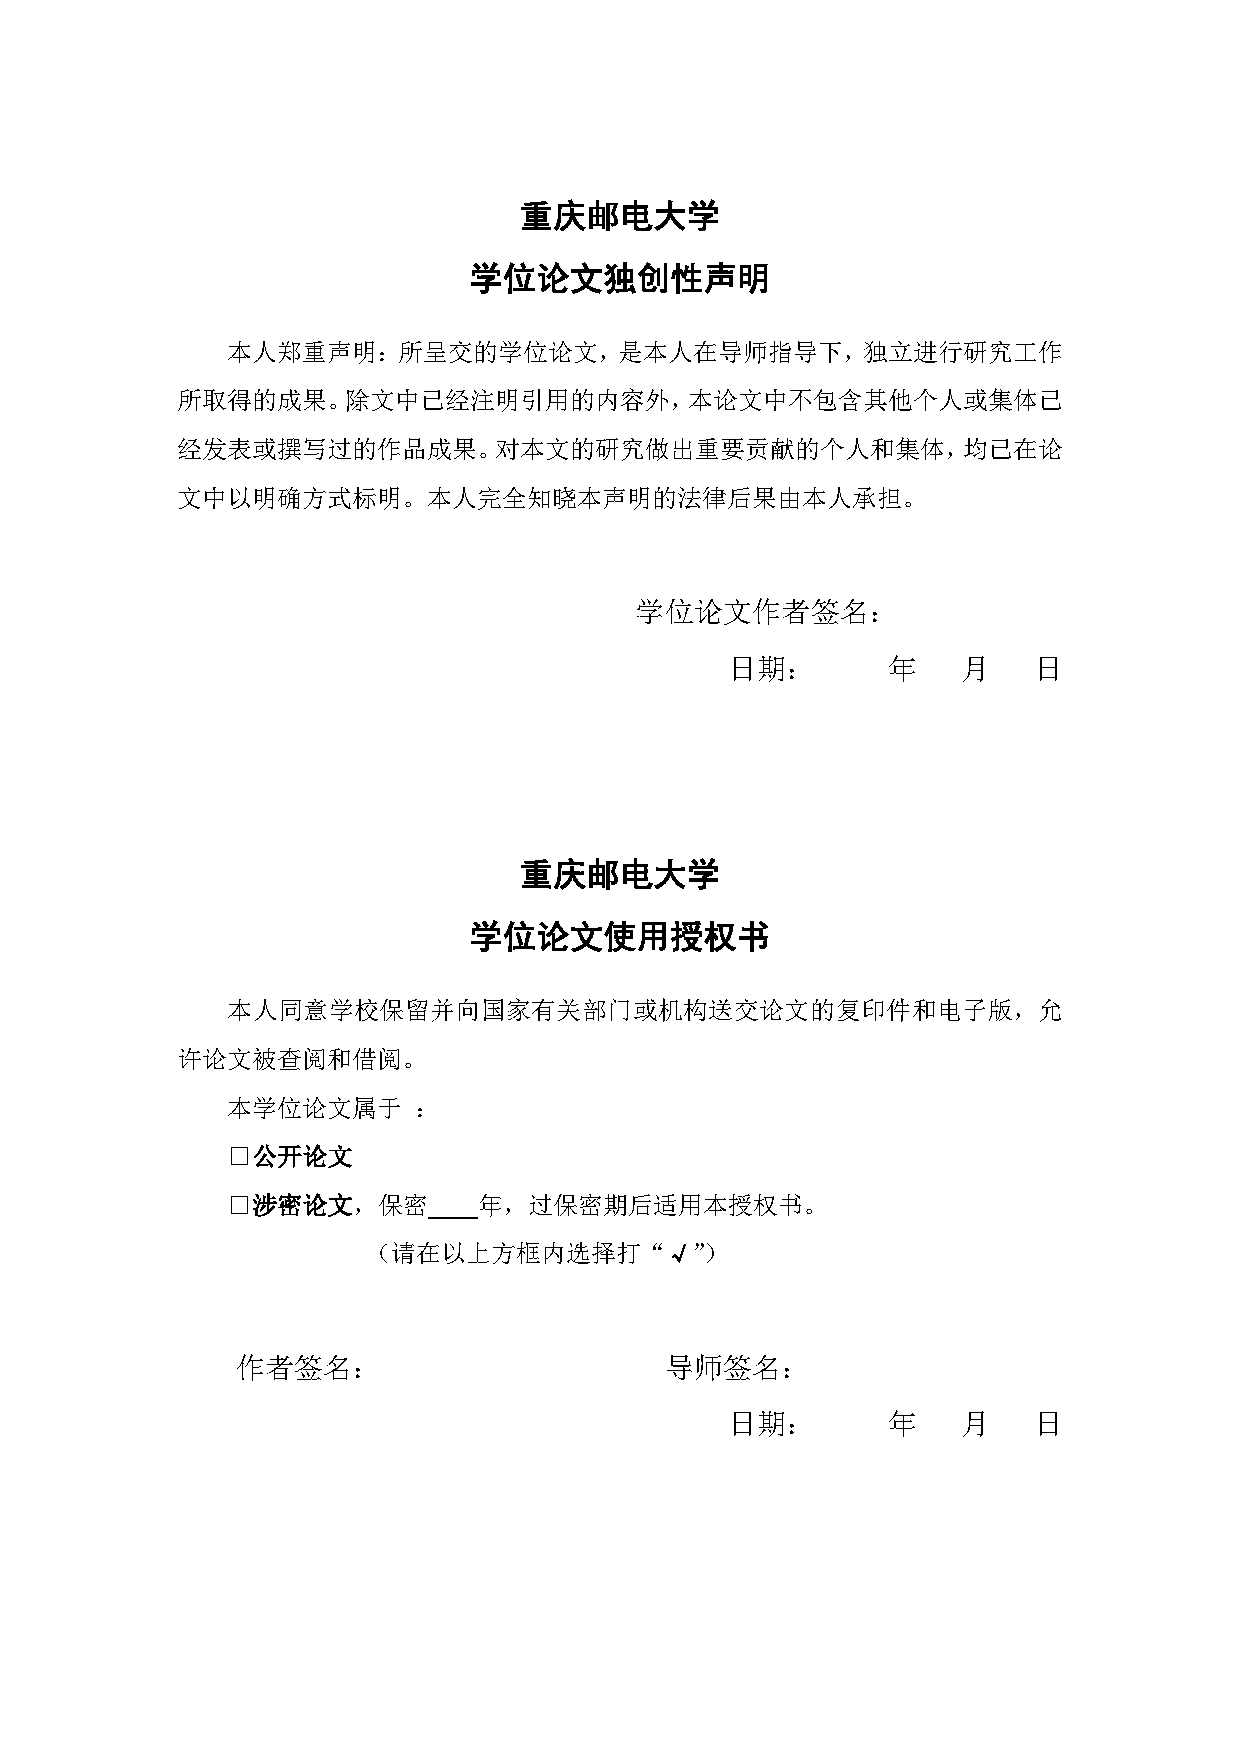
\includepdf{original.pdf}
\clearpage


\clearpage

%前序部分(中英文摘要,目录等,chapter后面不编号)
\frontmatter

%开始以大写罗马字母计页码
\pagenumbering{Roman}

\pagestyle{plain}
%页面格式
%\pagestyle{plain}

% 中文摘要页
%中文摘要,自行编辑内容



\chapter{摘\quad 要}
\xiaosi

当下深度学习技术在众多领域都展现了其应用潜力,在图像分类领域,随着模型结构的日益复杂,参数量逐渐提升,人们很难对图像分类模型给出的分类结果给出可靠的解释。显著图解释技术作为深度学习可解释工作的一个新兴分支,其研究目的是从输入图片中找到图像分类模型做出决策的依据成从而给出可视化的解释。但是当前的显著图解释技术普遍存在生成的原始显著图分辨率较低,无法精确定位目标关键特征等缺陷。因此本研究针对当前显著图解释技术存在的缺陷入手,研究如何提高显著图的分辨率,增加显著图的呈现的有效信息,提高显著图对图像分类神经网络决策结果的可视化解释能力。本研究的主要工作如下:

首先,本研究提出了一种针对基于卷积神经网络的图像分类模型的显著图解释方法。该方法通过将原始输入图片进行多尺度的放大并分别输入到图像分类模型当中,从图像分类神经网络的最后一层卷积层获取得到不同分辨率的特征图集合。再分别对目标类别的分数进行反向传播得到最后一层卷积层特征图对应的梯度矩阵。然后将不同分辨率特征图和梯度矩阵融合为和原始输入图片一样的分辨率并加权相加得到掩膜。将所有掩膜分别扰动原始输入图片后输入至图像分类模型当中得到目标类别的概率分数作为掩膜的权重。最后将所有掩膜和其对应的概率分数加权相乘得到最终的显著图。在三个公开的数据集( ILSVRC 2012数据集,PASCAL VOC数据集和COCO2014数据集)上进行定性和定量实验,该方法生成的显著图具有更高分辨率,能够更加精准地找到图像分类神经网络在输入图片中的决策依据,提供更加直观的可视化解释结果。

其次,针对目前显著图解释方法生成的原始显著图普遍低分辨率的情况,本研究提出了一种通用的显著图增强方法,可以直接应用在多数显著图解释方法上。该方法使用固定尺寸的滑动窗口对输入图片中的所有局部区域上采样到输入图片尺寸,然后将结果输入到选定的显著图解释方法中得到所有图片的针对特定类别的显著图和概率分数,最后将显著图下采样到输入图片对应位置上的窗口中,并乘以概率分数,即可得到具备更多细节的显著图。本研究将该方法应用在不同的显著图解释方法上,无论是量化指标还是直观评测都显示出该方法明显提升了其他显著图解释方法生成显著图的质量,从而证明该方法的有效性和可靠性。

最后,针对目前众多显著图生成方法实现复杂,难以直观对比不同方法生成的显著图质量优劣的问题,本研究设计并实现了一个显著图解释方法对比评测系统。
\\

\noindent\songti\textbf{关键词:}图像分类神经网络,深度学习可解释性,显著图,类激活映射

\clearpage


% 英文摘要页
%英文摘要,自行编辑内容




\chapter{ABSTRACT}
\xiaosi

Nowadays, deep learning technology has shown its application potential in many fields, and in the field of image classification, with the increasing complexity of the model structure and the gradual increase in the number of parameters, it is difficult to give reliable explanations for the classification results given by image classification models. The saliency map interpretation technique, as an emerging branch of deep learning interpretable work, aims to find the basis for the image classification model to make decisions from the input images, so as to give a visual interpretation. However, the current saliency map interpretation techniques generally have the defects of generating original saliency maps with low resolution and being unable to accurately locate the key features of the target. Therefore, in this thesis, we focus on the defects of the current saliency map interpretation technology to study how to improve the resolution of the saliency map, increase the effective information presented by the saliency map, and improve the ability of the saliency map to explain the visualization of the decision-making results of the image classification neural network. The main work of this thesis is as follows:

First, this thesis proposes a saliency map interpretation method for image classification model based on convolutional neural network. The method obtains a collection of feature maps with different resolutions from the last convolutional layer of the image classification neural network by zooming the original input image at multiple scales and inputting them into the image classification model separately. The gradient matrix corresponding to the feature maps of the last convolutional layer is obtained by backpropagating the scores of the target categories respectively. Then the different resolution feature maps and the gradient matrix are fused into the discriminant of the original input image and weighted to obtain the mask. All the masks are perturbed to the original input image and input to the image classification model to get the probability scores of the target categories as the weights of the masks. Finally, all the masks and their corresponding probability scores are weighted and multiplied to obtain the final saliency map. Qualitative and quantitative experiments on three publicly available datasets (ILSVRC 2012 dataset, PASCAL VOC dataset, and COCO 2014 dataset) show that the saliency maps generated by this method have higher resolution and can more accurately find out the decision basis of the neural network for image classification in the input images, and provide more intuitive visual interpretation of the results.


Second, in response to the generally low resolution of the original saliency maps generated by current saliency map interpretation methods, this thesis proposes a generalized saliency map enhancement method that can be directly applied to most saliency map interpretation methods. The method uses a fixed-size sliding window to up-sample all local regions in the input image to the input image size, and then inputs the results to the selected saliency map interpretation method to obtain category-specific saliency maps and probability scores for all images, and finally down-samples the saliency maps to the window at the corresponding position of the input image and multiplies them by the probability scores, which results in saliency maps with more details. In this thesis, the method is applied to different saliency map interpretation methods, and both quantitative indexes and intuitive evaluation show that the method significantly improves the quality of the saliency maps generated by other saliency map interpretation methods, thus proving the effectiveness and reliability of the method.

Finally, for the current existence of many saliency map generation methods to achieve complexity, it is difficult to intuitively compare the quality of saliency maps generated by different methods of the problem, this thesis designs and implements a saliency map interpretation method comparison evaluation system.
\\

\noindent\textbf{Keywords:} 
\begin{minipage}[t]{0.85\linewidth}
	Image Classification Neural Networks, Deep Learning Interpretability, Saliency Maps, Class Activation Mapping
\end{minipage}

\clearpage


% 目录
%\begin{spacing}{1.14}
\tableofcontents


\begingroup
\renewcommand*{\addvspace}[1]{}
%图目录
%\newcommand{\loflabel}{图}
%\renewcommand{\numberline}[1]{\loflabel~#1\hspace*{1em}}
\listoffigures

%表目录
%\newcommand{\lotlabel}{表}
%\renewcommand{\numberline}[1]{\lotlabel~#1\hspace*{1em}}
\listoftables
\endgroup

%\end{spacing}





%主要符号表


\chapter{主要符号表}



\begin{table}[h]
	\renewcommand{\arraystretch}{1.5}
	\centering
	\begin{tabular}{p{2cm}p{10cm}p{1.5cm}}
		\toprule[1.5pt]
		\makecell[l]{\songti\xiaosi\bfseries 符号}&\makecell[l]{\songti\xiaosi\bfseries 说明}&\makecell[c]{\songti\xiaosi\bfseries 页码}\\
		\hline
		\makecell[l]{\wuhao c}&\makecell[l]{\wuhao 电磁波的相平面速度}&\makecell[c]{\wuhao 10}\\
		\bottomrule[1.5pt]
	\end{tabular}
     
\end{table}

\clearpage

%缩略词表




\chapter{缩略词表}

\begin{table}[h]
	\renewcommand{\arraystretch}{1.5}
	\centering
	\begin{tabular}{p{2cm}p{8.5cm}p{3cm}}
		\toprule[1.5pt]
		\makecell[l]{\songti\xiaosi\bfseries 英文缩写}&\makecell[l]{\songti\xiaosi\bfseries 英文全称}&\makecell[l]{\songti\xiaosi\bfseries 中文全称}\\
		\hline
		\makecell[l]{\wuhao CQUPT}&\makecell[l]{\wuhao Chongqing University of Posts Telecommunications}&\makecell[l]{\wuhao 重庆邮电大学}\\
		\bottomrule[1.5pt]
	\end{tabular}
	
\end{table}

\clearpage

\clearpage

%% 开始章节写作,chapter后面开始编号,显示特定页眉页脚
\mainmatter
\pagenumbering{arabic}

%正文页眉避免英文全部大写
\renewcommand\thechapter{\arabic{chapter}}
\renewcommand{\chaptermark}[1]{\markboth{第 \thechapter 章 \ #1}{}}




% 第1章



\chapter{绪论}
\thispagestyle{others}
\pagestyle{others}
\xiaosi

\section{研究背景及意义}
当今的社会正处于智能化趋势的浪潮中,由深度学习理论所衍生的相关技术被广泛的应用在人们所熟知的各个领域,例如自然语言处理\textsuperscript{\cite{language}}、语音识别\textsuperscript{\cite{voice}}、图像分类\textsuperscript{\cite{image,simonyan2014very}}、目标检测\textsuperscript{\cite{od1,od2}}和语义分割\textsuperscript{\cite{sg1,sg2}}。在学术界和工业界的互相融合促进下,深度学习算法不断推陈出新,深度神经网络也不断进化并发展出适用与文字、图像、视频等信息介质的自动化识别和信息提取的高效的深度神经网络模型,许多相关领域深度神经网络模型已经是现代社会正常运转的不可或缺的一部分。

但是,当前主流的深度神经网络并不具备良好的可解释性,即便这些深度神经网络在各种测试任务下展现出了很高的准确率。例如在图像分类应用中,将待分类的图片送入训练好的深度神经网络会得到不同类别物体的置信概率分数,即便某一类别的置信概率分数是99.99\%,也无法得到深度神经网络做出这一决策的依据\textsuperscript{\cite{machine}},即该深度神经网络的输出结果并不具备可解释性。并且随着应用场景的复杂化多样化,深度神经网络结构日趋复杂,参数数量日趋庞大,这使得深度神经网络的“黑盒”特点变得更为突出。这种难以解释的黑盒特性使得深度神经网络在可靠性要求极高的领域,诸如医疗影像、自动驾驶、航空航天\textsuperscript{\cite{arospace}}等领域的应用就受到限制。

除此之外,上述的黑盒特性也会成为当前的深度神经网络的研究过程当中的“拦路虎”。研究者往往是将训练好的深度神经网络在既有的数据集上根据各种外部的量化指标评价训练效果,但是在实际应用过程当中,模型可能会对现实世界中某些特殊的数据或者人为恶意伪造的数据给出异常的结果。如果训练的深度神经网络不能对这些意外数据有着良好的鲁棒性,那么该神经网络的就不能得到人们的信任。因此这使得相关研究者必须从更加全面的角度判断深度神经网络的性能表现并且解释其训练的神经网络的结果输出,而不只是依赖单一的评价指标来判断神经网络的性能表现。

因此,从深度神经网络实际应用和可靠性的角度出发,都需要有适用于深度神经网络黑盒特性的可解释方法,所以许多研究人员将目光转移到深度神经网络的可解释性上,他们或试图从既有的深度神经网络内外寻找其的决策依据,或试图从原理上构建可解释的深度神经网络,这两类研究路径分别就是后解释(Post-hoc Explanation)\textsuperscript{\cite{post,post2}}的人工智能和自解释(Intrinsic Explanation)\textsuperscript{\cite{Intrinsic1,Intrinsic2,Intrinsic3,Intrinsic4,Intrinsic5,Intrinsic6}}的人工智能。

通过利用针对深度神经网络的可解释方法,不仅可以使得研究者和用户知道深度神经网络的决策依据,理解其中的决策机理,增强人对神经网络输出结果的信任程度,还可以使得研究者对神经网络的可靠性进行针对性的验证和测试。加强对深度神经网络可解释方法的研究有助于研究人员用更加全面且灵活双向的方式和神经网络进行交互,能做到“知其然并知其所以然”。可解释性的研究赋予了深度神经网络更多的可能性并加强了其可靠性。

本文主要聚焦于图像分类神经网络的可解释性研究,更加具体的是利用图像即显著图的方式来提供图像分类神经网络的可解释性,这是一种后解释的可解释研究,它能根据显著图中给出权值数据来解释图像分类神经网络的输出结果并判断其内部决策过程是否合理可靠。同时本文的研究侧重点在于不改变神经网络内部参数,仅利用既有训练好的深度神经网络模型来进行可解释性研究。既有的图像分类神经网络模型在工业界和学术界已经得到了大量的应用,并且拥有很好的性能表现,因此在不改变模型的前提下,本文的研究可以提供简单明了能直接使用的可解释方法,对已经训练完成模型的输出结果进行显著图分析解释,将单一的,不可解释的输出结果转变为直观明了的,可解释的图像结果,提高了模型的可靠性和可信任性。此外,显著图给出的分析结果可以帮助研究者有效分析模型是否学习到正确的特征,提供神经网络决策的关键依据。





\section{国内外研究现状}
\subsection{基于反向传播的显著图解释技术}
利用反向传播的机制来实现可视化解释是较早的一些工作所采用的方法。M D.Zeiler等人\textsuperscript{\cite{zeiler2014visualizing}}提出了一种基于反卷积的可视化方法,反卷积将特征值逆映射回了输入图片的像素空间,借此说明图片中的哪些像素参与激活了该特征值。在这项工作的基础上,导向反向传播方法\textsuperscript{\cite{springenberg2014striving}}提出在反向传播时通过抑制输入和梯度小于0的值,从而突出可视化目标的重要特征。DeepLIFT\textsuperscript{\cite{shrikumar2017learning}},LRP(Layer-wise Relevance Propagation)\textsuperscript{\cite{binder2016layer}}方法通过修改反向传播的规则,将输出层的贡献逐渐向下分配直到输入层,以此来获得输入图片中每个像素对输出相关性分数。K.Simonyan等人\textsuperscript{\cite{simonyan2014deep}}提出使用输入的梯度作为可视化解释的一种手段,这种方法认为输入的某些像素对网络的预测结果起到了主要作用,它直接计算网络输出的特定类别分数对输入的梯度,但是输入的梯度中包含明显的噪声,导致显著图可视化十分模糊。SmoothGrad方法\textsuperscript{\cite{smilkov2017smoothgrad}}和VarGrad方法\textsuperscript{\cite{adebayo2018local}}的原理都是共同的,它们向输入图片中多次添加噪声生成一组包含噪声的图片,通过平均化结果使得生成的显著性图更加平滑。为了解决梯度饱和问题,Sundararajan等人提出了一种积分梯度方法\textsuperscript{\cite{sundararajan2017axiomatic}},该方法结合了直接计算梯度和基于反向传播的归因技术DeepLIFT和LRP的分而治之的设计思想,满足敏感性和实现不变性的公理。这些研究虽然有坚实的理论基础,但是它们的可视化结果对于人类来说不容易理解,而且噪声较多。此外这些方法中许多是和具体类别不相干的,无法对指定类别给出显著图可视化解释结果。另外有研究\textsuperscript{\cite{adebayo2018sanity}}指出其中有些方法的可靠性是值得怀疑的,它们对深度神经网络的参数不敏感,即使网络没有经过训练也能得到相似的结果。

\subsection{基于类激活映射的显著图解释技术}
基于类激活映射的方法是目前被大量研究和应用的一种流行的方法。这类方法利用了卷积神经网络中靠近输出端的信息,这些信息中包含着和预测结果相关的丰富的类别信息,所以这类方法能够给出类别相关的显著图可视化解释。CAM\textsuperscript{\cite{zhou2016learning}}方法首先提出了将卷积神经网络的最后一层全局平均池化后得到权重和该层提取的特征图线性相乘后累加  从而生成显著图。Grad-CAM\textsuperscript{\cite{selvaraju2017grad}}对CAM方法进行了改进,无需修改网络结构,利用反向传播的梯度取均值作为权重。Grad-CAM++\textsuperscript{\cite{chattopadhay2018grad}}进一步改进了Grad-CAM,它对不同像素的梯度进行加权,生成的显著图中能将同一类别物体出现多次的情况给较好的展示出来;XGrad-CAM\textsuperscript{\cite{fu2020axiom}}通过分析敏感性和实现不变性公理采用了另一种加权方法来获得特征图的权重,它引入了特征图中的像素权重为对应梯度进一步加权。为了减少噪声的影响,Smooth Grad-CAM++\textsuperscript{\cite{omeiza2019smooth}},SS-CAM\textsuperscript{\cite{wang2020ss}}也采用了SmoothGrad\textsuperscript{\cite{smilkov2017smoothgrad}2}和VarGrad\textsuperscript{\cite{adebayo2018sanity}2}中的向输入图片中多次添加噪声的措施。Score-CAM\textsuperscript{\cite{wang2020score}}和Ablation-CAM\textsuperscript{\cite{ramaswamy2020ablation}}没有使用反向传播中的梯度作为特征图的权重,它们将前向传播中从最后一层卷积层获得的特征图作为掩膜来扰动输入图片,利用网络输出值或者下降值作为特征图的权重,这种方法有效避免了使用梯度而产生的噪声,取得了良好的效果。Relevance-CAM\textsuperscript{\cite{lee2021relevance}}将卷积神经网络中提取的特征图再分别输入到卷积神经网络中,对每张特征图的预测结果进行层间相关性传播(Layer-wise Relevance Propagation),得到对应的相关性图,将相关性图全局平均池化后作为特征的权重,该方法有效解决了之前的CAM方法对卷积神经网络中间层可视化解释不足的问题。CAMERAS\textsuperscript{\cite{jalwana2021cameras}}提出了将输入图片进行多尺度放大再输入到网络当中,将提取到的不同分辨率的特征图和梯度全部放大到和原图分辨率一样。然而,基于类激活映射的方法只针对卷积神经网络进行设计,无法便捷的迁移到其他网络当中,比如基于Transformer的图片分类神经网络模型。


\subsection{基于扰动的显著图解释方法}
基于扰动的显著图可视化方法最突出的优点便是这种方法基本只关心网络的输入和输出,可以在不同结构网络轻松的应用,即使这些网络中的细节千差万别。Zeiler等人\textsuperscript{\cite{zeiler2014visualizing}2}使用一个固定形状的方块来对输入图片进行扰动,观察输出变化从而找到对模型而已输入图片中最重要的部分。SHAP方法\textsuperscript{\cite{lundberg2017unified}}使用了Shapley值,计算不同输入像素在是否存在的情况下对网络预测结果的影响,公平分配贡献度给这些像素点。LIME\textsuperscript{\cite{ribeiro2016should}}方法通过在较小的范围内扰动输入图片,得到输出结果,利用输入数据和输出数据重新训练一个可解释的代理模型去逼近黑盒模型在局部的决策边界,从而获得不同特征的重要性。RISE\textsuperscript{\cite{petsiuk2018rise}}利用蒙特卡洛方法随机生成的数量巨大的掩膜来扰动输入图片,将模型对特定类别输出概率作为的权重,再将多个所有掩膜加权相乘得到可视化结果。有研究提出了基于机器学习的方法,将掩膜作为优化对象,通过定义限制掩膜的损失函数,不断迭代从而找到最优的掩膜。在此基础上,R.Fong等人\textsuperscript{\cite{fong2019understanding}\cite{fong2017interpretable}}提出通过限制搜索区域,重新设计损失函数,达到了很好的效果。基于扰动的可视化算法因为能够对模型预测结果进行直接观察,所以可以较为真实的反映模型决策机制。但是,这种类型算法往往需要多次迭代,需要付出高额的计算成本

\section{论文研究的主要内容}
本文的主要研究内容是探究当前图像分类神经网络的预测结果的可解释性,具体而言是生成显著图来赋予输入图片中每个像素一个权值来探究输入图片中物体特征对图像分类神经网络的预测结果的重要程度。利用显著图可以直观呈现图像分类神经网络对目标类别的判别依据,为用户提供可视化的解释。  

本文是基于图像分类神经网络的显著图解释研究,并侧重于提升生成显著图的分辨率,提高显著图对重要特征的定位能力。具体而言本文提出了两种创新方法。

(1)本文提出了一种新的方法,可以针对基于卷积神经网络的图像分类模型的决策结果生成高分辨率的显著图。该方法采用多尺度放大原始输入图像,并将其输入到图像分类模型中。通过从最后一层卷积层获取不同分辨率的特征图集合,并对目标类别的分数进行反向传播,得到最后一层卷积层特征图对应的梯度矩阵。接着,将不同分辨率的特征图集合和梯度矩阵集合融合为原始输入图像的分辨率,并进行加权相加以生成掩膜。将所有掩膜分别应用于扰动原始输入图像,并输入到图像分类模型中,以获取目标类别的概率分数作为掩膜的权重。最后,对所有掩膜和其对应的概率分数进行加权相乘,生成最终的显著图。在ILSVRC 2012数据集\textsuperscript{\cite{ILSVRC}}、PASCAL VOC数据集\textsuperscript{\cite{pascal}}和COCO2014数据集\textsuperscript{\cite{coco}}上进行了定性和定量实验,结果显示该方法生成的显著图具有更高的分辨率,能够更准确地揭示图像分类神经网络在输入图像中的决策依据,提供更直观的可视化解释结果。

(2)本文提出了一种通用的显著图增强方法,旨在解决当前显著图解释方法生成低分辨率显著图的问题。该方法适用于多种显著图解释方法,可以在不改变原有方法内部计算流程的情况下,达到提高显著图分辨率,增强显著图对特征的定位能力的效果。该方法通过使用固定尺寸的滑动窗口对输入图像的局部区域进行上采样,并将结果输入到选定的显著图解释方法中,得到针对特定类别的显著图和概率分数。随后,将显著图下采样到输入图像对应位置的窗口中,并乘以概率分数,生成具备更多细节高分辨率的显著图。该方法在不同显著图解释方法上的应用结果表明,无论是通过量化指标还是直观评测,都显示出显著图质量得到明显提升。

\section{论文组织结构} 
本文一共分为六个章节,其组织结构如下:

第1章,绪论。本章介绍了当前深度学习可解释性的研究背景并引出本文的基于图像分类神经网络的显著图解释研究内容;然后介绍国内外当前研究现状并重点介绍了三类显著图解释方法和其发展历程,接着围绕当前显著图解释方法的存在缺陷引出本文的重点研究内容即提高显著图分辨率,增强显著图对重要特征的定位能力,提供高质量的可视化解释。

第2章,相关理论介绍。该章节对本文使用的两种图像分类神经网络架构:卷积神经网络和Transformer架构进行了简要介绍;然后重点介绍了当前几种著名的显著图解释方法的背后的原理和其计算流程。

第3章,基于输入图片多尺寸放大的卷积神经网络显著图解释方法。该章节介绍本文为了解决当前针对卷积神经网络显著图解释方法生成的显著图分辨率较低,特征定位模糊的问题,提出了一种能生成高分辨率,特征定位更为准确的显著图解释方法并详细介绍了算法流程。然后设计实验通过在多个数据集上进行不同维度的实验评价,综合多个评价指标验证了提出方法的有效性。

第4章,一种通用的基于二维滑动窗口和放大的图像分类神经网络显著图解释增强方法。该章节针对当前显著图解释方法普遍存在的生成显著图分辨率低的问题,提出了一种简单易于实施的通用的显著图解释方法增强方法并详解介绍了其中的算法流程包括二维滑动窗口的算法过程。然后本章设计了实验,通过将本文提出的增强方法应用在多种显著图解释方法上,并选用了不同架构的图像分类神经网络和多种数据集进行多个维度的测试,分析测试结果显示本章的增强方法具有明显提升效果。

第5章,显著图解释方法对比评测系统。本章针对当前存在的多种显著图解释方法实施算法复杂对比困难的情况开发了一个显著图解释方法对比评测系统。本章依次介绍了系统需求分析、开发环境及相关开发技术、系统设计和系统展示。

第6章,总结和展望。本章对本文的所有研究内容和创新点进行了总结,并对当前深度学习可解释性领域和显著图解释方法进行了分析展望,说明未来可能存在的研究进展和突破。



\clearpage

% 第2章



\chapter{相关理论介绍
}
\thispagestyle{others}
\pagestyle{others}
\xiaosi

\section{引言}
解释深度神经网络引起了越来越多的关注,因为它有助于理解网络的内部机制以及网络做出特定决策的原因。在计算机视觉领域中,可视化和理解深度神经网络最流行的方法之一是生成与网络决策相关的显著区域的显著性图。许多深度神经网络相关的可解释方面的研究和方法都可以在图像分类神经网络上生成显著图。显著图生成的质量可以直观反映不同可解释或者可视化算法的优劣,此外显著图还可以作为图像弱监督分割和目标的定位的一种手段,因其可以反映目标物体在图像中的空间位置而且其只需要训练好的图像分类神经网络即可完成任务。


%一些早期的研究单纯通过反向传播的梯度差异来生成显著图描述图像分类模型在输入图片中感兴趣的区域,后来
深度神经网络的可解释方面的研究是在最近十年才逐渐兴起并收到关注的,在计算机视觉领域,基于深度卷积神经网络的图像分类模型是较早受到研究的,研究者试图从参数量庞大的深度卷积神经网络中找到输出结果和在输入图片中对应的依据。也有一些研究者将图像分类神经网络看作是一个黑盒,通过各种手段扰动输入图片观测输出结果变化来生成显著图。随着Transformer架构异军突起,基于Transformer架构的图像分类神经网络的可解释性也逐渐受到关注和研究,也已经由研究者设计了针对Transformer架构的反向传播归因机制,该机制在计算机视觉领域也能生成效果良好的显著图。上述的深度神经网络可解释研究生成的显著图较少关注显著图生成的质量和对关键特征的定位能力,本文的显著图解释研究专注于对显著图生成质量的改善和相关显著图解释算法的改善。

接下来本章首先介绍图像分类神经网络的主流架构概念包括基于卷积神经网络 的和基于Transformer架构的,然后介绍五种著名的深度学习可解释算法,这些算法在图像分类神经网络上也能生成显著图,后续实验当中这五种算法也会用来作为对比。

\section{卷积神经网络}
卷积神经网络(Convolutional Neural Networks,CNNs)一种特殊类型的神经网络,特别适合于计算机视觉应用\textsuperscript{\cite{image}1-2}。它的设计灵感来源于生物学上对动物视觉皮层的研究,旨在模拟人类视觉系统的工作原理。卷积神经网络的结构包括卷积层、池化层和全连接层,这些层的组合使得CNNs能够有效地处理图像识别、分类和分割等任务。有两个关键的设计思想推动了卷积架构在计算机视觉中的成功。首先,卷积神经网络利用图像的二维结构和一个邻域内的像素通常高度相关的事实。因此,ConvNets避免使用所有像素单元之间的一对一连接(即大多数神经网络的情况),而倾向于使用分组的局部连接。此外,ConvNet架构依赖于特征共享,因此每个通道(或输出特征映射)都是由在所有位置使用相同滤波器进行卷积生成的,如图\ref{fig:conv1}所示。与标准神经网络相比,卷积神经网络的这一重要特征导致其架构依赖的参数要少得多。其次,卷积神经网络还引入了一个池化步骤,该步骤提供了一定程度的平移不变性,使体系结构较少受到位置变化的影响。另外,池化还允许网络逐渐看到更大的输入部分,这要归功于网络接受视野的增加。随着网络深度的增加,接受视野的大小增加(同时输入分辨率减小),使得网络能够表示输入的更抽象特征。例如,在目标识别任务中,卷积神经网络的层从关注物体的边缘开始,逐渐覆盖整个物体的各个部分,最终从更高层次上覆盖整个物体。

\begin{figure}[h]
	\centering 
	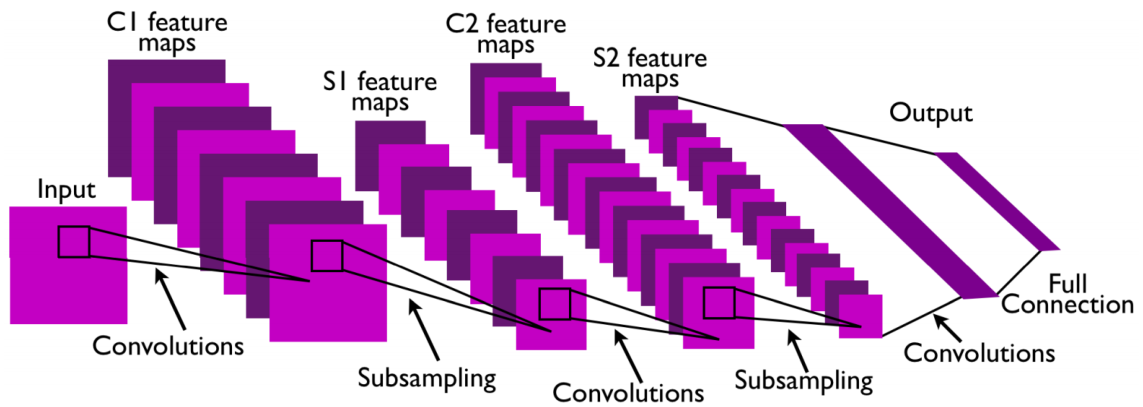
\includegraphics[width=15cm]{fig/ch2/conv1.png}
	\bicaption[\xiaosi 标准卷积网络结构示意图]{\wuhao 标准卷积网络结构示意图}{\wuhao Illustration of the structure of a standard convolutional network}
	\label{fig:conv1}
\end{figure}

卷积神经网络的核心是卷积层,它通过卷积操作提取输入图像的特征。卷积操作是一种线性、平移不变的操作,它通过在输入信号上进行局部加权组合来捕获不同的特征。卷积操作的参数是卷积核,不同的卷积核可以捕获图像的不同特征,例如边缘、纹理和形状等。卷积层的输出被送入激活函数进行非线性变换,以增加网络的表达能力。

除了卷积层,池化层也是卷积神经网络中的重要组成部分。池化层通过对卷积层的输出进行下采样,减少特征图的尺寸,同时保留最显著的特征。这有助于使网络对输入的位置变化具有一定的不变性,同时减少了参数数量,提高了计算效率。

全连接层通常位于网络的末尾,用于将卷积层和池化层提取的特征映射转换为最终的分类或回归结果。全连接层将所有特征进行组合,最终输出网络对输入的预测结果。


\section{基于Transformer的图像分类神经网络}
Transformer\textsuperscript{\cite{bengio2013representation}}是一种基于自注意力机制的深度学习模型架构,最初由A.Vaswani等人于2017年提出\textsuperscript{\cite{vaswani2017attenion}},被广泛应用于自然语言处理任务,如机器翻译、文本生成和语言建模等。相较于传统的循环神经网络(RNN)和卷积神经网络(CNN),Transformer在处理长距离依赖性和并行计算方面具有显著优势,成为了当今深度学习领域的研究热点。

Transformer模型的核心思想是完全基于注意力机制来实现信息的传递和组合。在传统的神经网络结构中,信息的传递是通过固定的层次顺序进行的,而Transformer则引入了自注意力机制,使得模型可以在不同位置之间建立动态的注意力联系。这种注意力机制使得模型能够更好地捕捉输入序列中不同位置之间的依赖关系,从而提高了模型在处理长距离依赖性任务时的性能。

如图\ref{fig:vit1}所示,Transformer模型由编码器和解码器两部分组成,每部分都包含多层的注意力机制模块。在编码器中,输入序列首先通过一个自注意力层,然后再通过一个全连接前馈神经网络层。在自注意力层中,每个输入位置都可以与其他位置建立注意力联系,从而使得模型能够同时考虑到整个输入序列的信息。在解码器中,除了编码器的结构外,还引入了一个额外的注意力层,用来对编码器的输出进行进一步处理。

除了自注意力机制,Transformer还引入了位置编码来表示输入序列中不同位置的信息。由于Transformer没有显式的循环结构,无法像RNN一样自然地捕捉序列中的位置信息,因此位置编码的引入可以帮助模型更好地理解输入序列中不同位置的相对位置关系。

另一个Transformer模型的重要特点是其并行计算能力。由于自注意力机制的特性,Transformer可以高效地进行并行计算,加速模型的训练和推理过程。这使得Transformer在处理大规模数据和长序列任务时具有明显的优势。


\begin{figure}[h]
	\centering 
	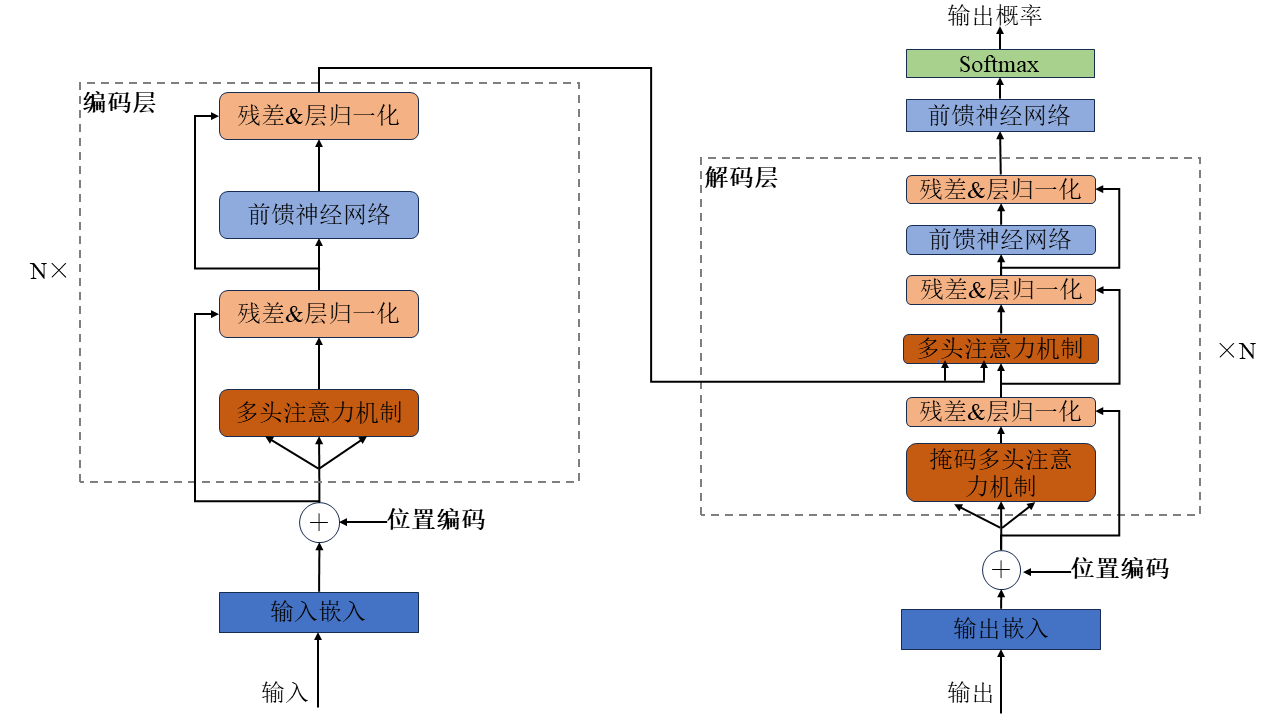
\includegraphics[width=15cm]{fig/ch2/vit1.png}
	\bicaption[\xiaosi Transformer结构示意图]{\wuhao Transformer结构示意图}{\wuhao Illustration of the structure of Transformer}
	\label{fig:vit1}
\end{figure}

\subsection{多头自注意力机制}
多头注意力机制是一种用于增强神经网络模型对输入序列的表示能力的技术。它通过将注意力机制应用于多个头部(head)来并行处理不同的注意力表示,从而提高模型的泛化能力和性能。多头注意力机制最早由Vaswani等人在Transformer模型中提出,并在自然语言处理领域取得了巨大成功。

多头注意力机制的基本原理是将输入序列分别映射到多个不同的查询、键和值空间,并通过计算每个头部的注意力权重来融合不同的信息。具体来说,多头注意力机制可以表示为以下公式:
\begin{equation}
	\text{MultiHead}(Q, K, V) = \text{Concat}(\text{head}_1, ..., \text{head}_h)W^O
\end{equation}



其中,$Q, K, V$分别表示输入序列的查询、键和值,$h$表示头部的数量,$\text{head}_i$表示第$i$个头部的注意力表示,$W^O$是输出权重矩阵。

在多头注意力机制中,每个头部都有自己的查询、键和值权重矩阵,通过线性变换将输入序列映射到不同的空间。然后,每个头部分别计算注意力权重,并将不同头部的注意力表示进行拼接,最后通过输出权重矩阵$W^O$融合多个头部的信息。

多头注意力机制的优势在于可以提高模型对不同部分的关注度,从而更好地捕捉输入序列中的重要信息。通过并行计算多个头部的注意力表示,模型可以更好地处理长距离依赖关系和复杂的序列结构,提高模型的泛化能力和性能。除了在Transformer模型中应用多头注意力机制,它还被广泛应用于其他神经网络模型中,如BERT\textsuperscript{\cite{kenton2019bert}}、GPT\textsuperscript{\cite{floridi2020gpt}}等。在自然语言处理、计算机视觉等领域,多头注意力机制已成为提高模型性能的重要技术之一。
 
\subsection{编码器}
Transformer模型是一种基于注意力机制的神经网络模型,由编码器和解码器组成,广泛应用于自然语言处理领域。编码器是Transformer模型的核心组件之一,它负责将输入序列转换成隐藏表示,提供给解码器进行生成输出序列。编码器由多个编码器层堆叠而成,每个编码器层内部包含多头自注意力机制和前馈神经网络。

编码器的每一层都包含两个子层,分别是多头自注意力机制和前馈神经网络。下面分别介绍编码器每一层的计算过程:

1. 多头自注意力机制(Multi-Head Self-Attention):

多头自注意力机制是编码器每一层的第一个子层,用于计算输入序列的注意力表示。具体的计算过程可以表示为以下公式:

\begin{equation}
	\text{Attention}(Q, K, V) = \text{softmax}\left(\frac{QK^T}{\sqrt{d_k}}\right)V
\end{equation}

其中,$Q, K, V$分别表示输入序列的查询、键和值,$d_k$表示注意力头部的维度。在多头自注意力机制中,将输入序列分别映射到多个不同的查询、键和值空间,并通过计算每个头部的注意力权重来融合不同的信息。

2. 前馈神经网络(Feed-Forward Neural Network):

前馈神经网络是编码器每一层的第二个子层,用于对注意力表示进行非线性变换。具体的计算过程可以表示为以下公式:

\begin{equation}
	\text{FFN}(x) = \text{ReLU}(xW_1 + b_1)W_2 + b_2
\end{equation}


其中,$x$表示输入的注意力表示,$W_1, b_1, W_2, b_2$分别表示两个线性变换的权重和偏置。前馈神经网络通过两个线性变换和ReLU激活函数来对注意力表示进行非线性变换,从而提高模型的表征能力。

在编码器中,每个编码器层都包含多头自注意力机制和前馈神经网络这两个子层,通过堆叠多个编码器层来构建整个编码器。每个编码器层都可以表示为以下公式:
\begin{equation}
	\text{EncoderLayer}(x) = \text{FFN}(\text{Attention}(x) + x)
\end{equation}

其中,$x$表示输入序列的隐藏表示,$\text{Attention}(x)$表示多头自注意力机制的输出,$\text{FFN}(\cdot)$表示前馈神经网络的输出。通过将多头自注意力机制的输出和原始输入序列相加,并通过前馈神经网络进行非线性变换,编码器可以逐层提取输入序列的特征表示。

在Transformer模型的编码器中,除了多头自注意力机制和前馈神经网络之外,还包括残差连接和层归一化这两个重要的组件。残差连接和层归一化在每个编码器层中都起着重要的作用,有助于提高模型的训练稳定性和加速收敛。下面分别介绍这两个组件的作用和公式表达:


3. 残差连接(Residual Connection):

残差连接是指将输入序列的隐藏表示与经过子层处理后的表示进行相加,从而形成残差连接。这样的设计有助于减轻梯度消失和梯度爆炸的问题,提高模型的训练效果。残差连接的计算公式可以表示为:

\begin{equation}
	\text{Residual}(x, \text{Sublayer}(x)) = x + \text{Sublayer}(x)
\end{equation}


其中,$x$表示输入序列的隐藏表示,$\text{Sublayer}(x)$表示经过子层处理后的表示。通过残差连接,编码器每一层的输出可以保留原始输入序列的信息,同时加入子层处理后的新信息,从而提高模型的表征能力。

4. 层归一化(Layer Normalization):

层归一化是一种对神经网络中每一层输出进行归一化的技术,有助于加速模型的收敛和提高模型的泛化能力。在编码器的每个子层(包括多头自注意力机制和前馈神经网络)后都会应用层归一化操作。层归一化的计算公式可以表示为:
\begin{equation}
	\text{LayerNorm}(x) = \gamma \odot \frac{x - \mu}{\sqrt{\sigma^2 + \epsilon}} + \beta
\end{equation}


其中,$x$表示输入序列的隐藏表示,$\gamma$和$\beta$分别表示学习到的缩放因子和偏置项,$\mu$和$\sigma$分别表示输入的均值和标准差,$\epsilon$是一个很小的常数,避免分母为零。层归一化通过对每一层的输出进行归一化,有助于减少内部协变量转移,提高模型的训练效果。

\subsection{解码器}
在Transformer模型中,解码器是用于生成目标序列的部分,与编码器相对应。解码器由多个解码器层组成,每个解码器层包含掩码多头自注意力机制、多头自注意力机制、层归一化、残差连接、前馈神经网络。此处重点介绍一下掩码多头自注意力机制(Masked Multi-Head Self-Attention)。

在Transformer模型中,掩码多头自注意力机制是解码器中的关键组件之一,它允许解码器在生成目标序列时关注目标序列中的不同位置,并避免未来信息的干扰。掩码多头自注意力机制包含多个注意力头,每个头都学习不同的注意力权重,然后将它们合并起来以获得最终的注意力表示。

在掩码多头自注意力机制中,给定一个输入序列$X = \{x_1, x_2, ..., x_n\}$,我们首先通过线性变换得到查询(Query)、键(Key)和值(Value)的表示:
\begin{equation}
Q = XW^Q, \ K = XW^K, \ V = XW^V
\end{equation}
其中$W^Q, W^K, W^V$是学习的权重矩阵。接下来,计算每个注意力头的注意力分数$A_i$:
\begin{equation}
A_i = \text{softmax}(\frac{Q_iK_i^T}{\sqrt{d_k}})
\end{equation}
其中$Q_i, K_i$表示第$i$个注意力头的查询和键,$d_k$是键的维度。然后,将每个注意力头的注意力分数与值相乘并加权求和,得到最终的输出表示:
\begin{equation}
\text{MultiHead}(Q, K, V) = \text{Concat}(\text{head}_1, ..., \text{head}_h)W^O
\end{equation}
其中$\text{head}_i = \text{Attention}(QW_i^Q, KW_i^K, VW_i^V)$表示第$i$个注意力头的输出,$W^O$是最终的输出权重矩阵。

在掩码多头自注意力机制中,为了避免未来信息的泄露,会对注意力分数进行掩码操作。具体来说,在计算注意力分数时,会将当前位置之后的信息屏蔽掉,以确保模型只能使用当前位置之前的信息。在实际操作中是将输入矩阵加上一个上三角矩阵,该上三角矩阵元素为无穷大。这种掩码操作有助于解码器在生成目标序列时保持因果关系,不受未来信息的影响。

通过掩码多头自注意力机制,解码器可以有效地关注目标序列中的不同部分,并根据输入序列和先前生成的部分序列调整生成的单词,从而实现对目标序列的准确生成。
\subsection{应用于图像分类领域的Transformer}
Transformer 技术最初是为了处理自然语言处理任务而设计的,但随着其出色的性能和可扩展性,人们开始将 Transformer 技术应用于其他领域,包括图像分类。虽然传统的卷积神经网络(CNN)在图像分类任务中表现出色,但 Transformer 在图像分类领域也展示出了很好的潜力。

在图像分类领域应用 Transformer 技术的一个主要方法是 Vision Transformer(ViT)\textsuperscript{\cite{dosovitskiy2020image}}。ViT 将输入的图像像素视为序列化的数据,然后利用 Transformer 模型来对序列化的图像数据进行处理。ViT 的基本架构如下:

图像块划分:将输入图像分成固定大小的图像块(patches),每个图像块将被视为一个 token。
输入嵌入层:将每个图像块映射为一个向量表示。
位置编码:为每个图像块的向量表示添加位置编码,以保留图像块之间的位置信息。
Transformer 编码器:使用 Transformer 模型对序列化的图像数据进行处理,包括多层的自注意力机制和前馈神经网络。
分类头:将 Transformer 的输出通过一个全连接层进行分类,得到图像的类别预测。

ViT 在图像分类领域的应用有以下优点:可扩展性:Transformer 模型的自注意力机制使得 ViT 能够捕捉图像中的全局信息,而不受卷积核大小的限制。灵活性:ViT 可以处理不同尺寸的图像,而无需调整网络结构。泛化能力:ViT 在处理小样本数据集时表现较好,因为 Transformer 模型具有强大的表示学习能力。ViT的结构如图\ref{fig:vit2}所示。

\begin{figure}[h]
	\centering 
	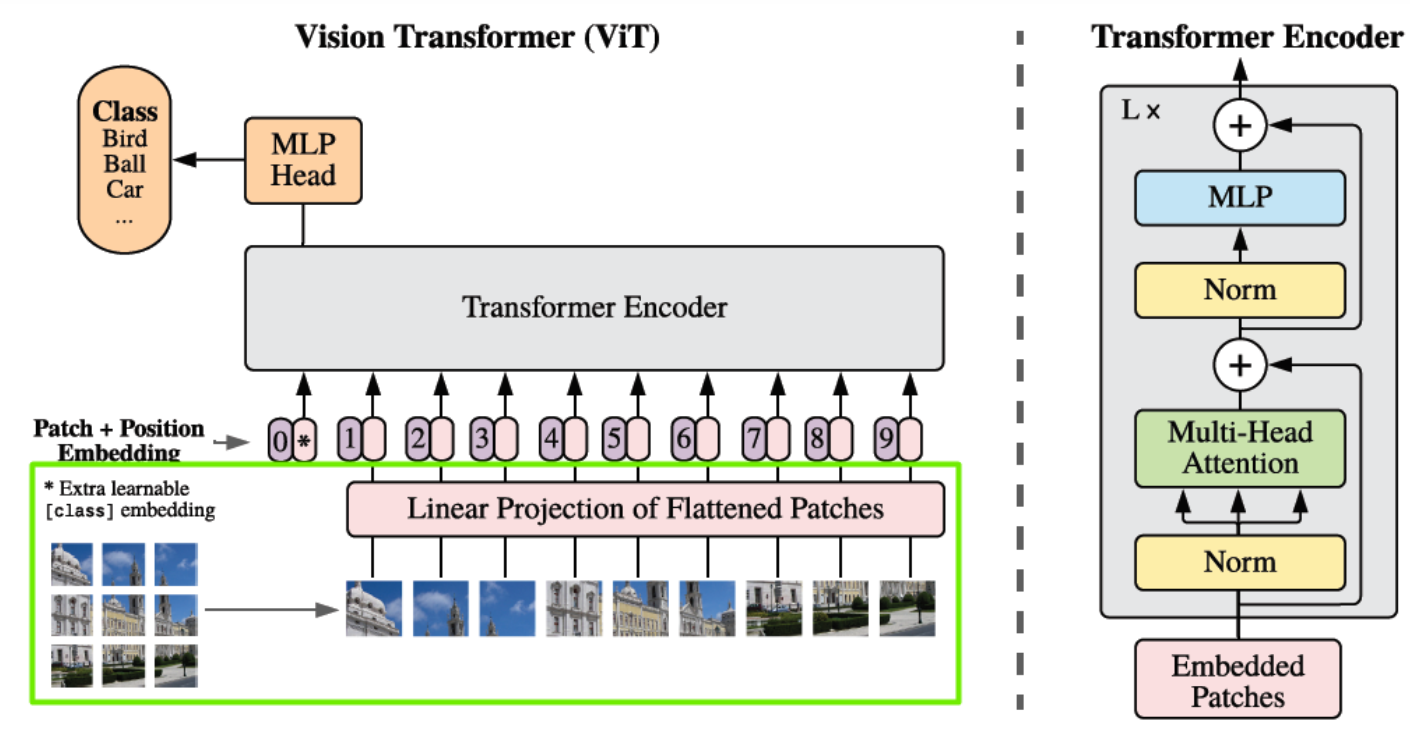
\includegraphics[width=15cm]{fig/ch2/vit2.png}
	\bicaption[\xiaosi ViT结构示意图]{\wuhao ViT结构示意图}{\wuhao Illustration of the structure of ViT}
	\label{fig:vit2}
\end{figure}


\section{常见的显著图解释方法}
本节将会介绍五种著名的显著图解释方法,包括Grad-CAM\textsuperscript{\cite{selvaraju2017grad}}、Grad-CAM++\textsuperscript{\cite{chattopadhay2018grad}}、Score-CAM\textsuperscript{\cite{wang2020score}}、LRP\textsuperscript{\cite{binder2016layer}}和Transformer attribution\textsuperscript{\cite{chefer2021transformer}}。本节将会介绍这五种方法的具体理论依据,各自的应用条件和算法流程。 
\subsection{Grad-CAM}\label{sub:gradcam}
Grad-CAM(Gradient-weighted Class Activation Mapping)是一种用于解释深度学习模型的方法,它能够生成图像级别的重要区域热力图,从而帮助理解模型的决策过程。Grad-CAM的主要优点是它不需要对模型进行修改,可以应用于任何卷积神经网络模型,并且能够提供直观的可视化结果。

Grad-CAM的核心思想是利用模型的梯度信息和特征图信息来推导出图像中哪些区域对于模型的分类决策最为关键。在深度学习模型中,每个卷积层都可以看作是对输入图像进行特征提取的过程,因此可以通过分析梯度信息来了解哪些特征对于模型的分类决策起到了关键作用。之前的一些研究已经断言,卷积神经网络的更深层表征捕获了更高层次的视觉结构\textsuperscript{\cite{bengio2013representation,mahendran2016visualizing}}。此外,卷积层自然地保留了在全连接层中丢失的空间信息,因此Grad-CAM的作者认为最后一层卷积层在高级语义和详细空间信息之间有良好的表现。因此Grad-CAM使用流入卷积神经网络最后一个卷积层的梯度信息,为每个神经元分配一个特定感兴趣的决策的重要性值。虽然Grad-CAM的技术相当通用,因为它可以用来解释深度网络任何层的激活,但是一般来说它用来可视化解释输出层做的决定。

\begin{figure}[h]
	\centering 
	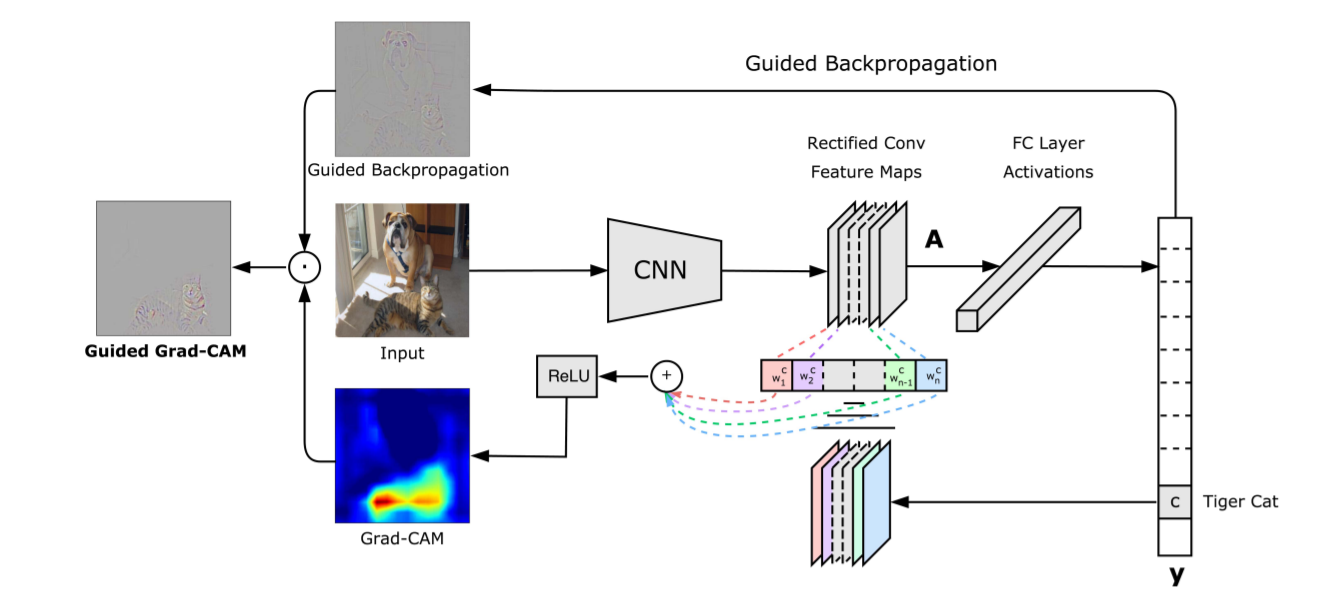
\includegraphics[width=15cm]{fig/ch2/gradcam1.png}
	\bicaption[\xiaosi Grad-CAM流程示意图]{\wuhao Grad-CAM流程示意图}{\wuhao Pipeline of  Grad-CAM}
	\label{fig:gradcam1}
\end{figure}

下面详细解释一下Grad-CAM的计算过程。若假设$I \in \mathbb{R}^{3\times H \times W}$是输入图片, $\mathcal{F}$是预训练好的基于卷积神经网络的图像分类模型,$\mathcal{F}_c(I)$ 表示输入图片是$I$的情况下模型$\mathcal{F}$输出的关于类别索引$c$的分数(该分数未经softmax函数)。对于给定的模型$\mathcal{F}$卷积层$l$,在图片$I$输入到模型$\mathcal{F}$前向传播过程中可以从卷积层$l$提取特征图集合$\overset{*}{\bm{A}}$。为了获取具有类别区分性的显著图,Grad-CAM首先需要计算关于类别$c$的梯度,为了得到 $\mathcal{F}_c(I)$ 相对于 第$k$张特征图 $A^k \in \overset{*}{\bm{A}}$ 的梯度,我们可以对 $\mathcal{F}_c(I)$ 进行反向传播。为了得到每个特征图的重要性权重,梯度会在高度和宽度两个维度上进行全局平均。
\begin{equation}
	w^c_k=\frac{1}{m\times n}\sum_{i=1}^{m}\sum_{j=1}^{n}\frac{\partial \mathcal{F}_c(I)}{\partial A_{ij}^k(I)}
	\label{eq:gradcam_wk}
\end{equation}
式子\ref{eq:gradcam_wk}表示了特征图集合中特征图$A^k$的权重计算方式,其中,$A_{ij}^k$ 表示 第$k$张特征图中 第$i$ 行和 第$j$ 列的值,$m$ 和 $n$ 分别是梯度矩阵的宽度和高度。$w^c_k \in \overset{*}{\bm{W}}$ 是 第$k$张 特征图的权重。$\overset{*}{\bm{W}}$是大小为$K$的一维向量,$K$是$\overset{*}{\bm{A}}$的通道数。


$w^c_k $的含义表示第$k$张特征图在后续计算中对输出分数$\mathcal{F}_c(I)$的贡献程度。最后将每张特征图和其权重相乘然后将相乘结果进行线性组合,最后通过ReLU函数即可得到Grad-CAM的显著图。具体计算方式如下所示:
\begin{equation}
	L_{Grad-CAM}=ReLU(\sum_K(w^c_k A^k))
	\label{eq:gradcam}
\end{equation}
需要注意的是注意,这会产生一个与特征图$A^k$尺寸大小相同的原始显著图,若需要将其展示重叠在输入图片上,应该将其进行上采样。还有就是ReLU函数应用于显著图的线性组合,是因为Grad-CAM只对感兴趣的类别有积极影响的特征感兴趣,即类别索引$c$所代表的类别。原始显著图中为负值的像素可能属于图像中的其他类别。若没有这个ReLU函数,显著图中会将其他不相干的类别进行凸显。图\ref{fig:gradcam1}简要展示了Grad-CAM的工作流程。


\subsection{Grad-CAM++}
在原始的CAM\textsuperscript{\cite{zhou2016learning}}方法中每张特征图的权重$w^c_k$是通过最后一层卷积层生成的特征图来训练线性分类器来获得的,但是其局限是必须使用全局平均池化层,需要重新训练模型,Grad-CAM解决了这一问题,通过最后的类别分数反向传播对最后一层卷积层的特征图求导,利用单个梯度矩阵的平均值来得到单张特征图权重,但是这会导致其对于某张特征图加权值过大从而将其他包含目标物体特征的特征图权值过小,从而在最后生成的显著图上忽略关键的特征。图\ref{fig:gradcampp1}举例说明了这一现象,如图所示,图中黑色方块部分表示目标物体在图中二维空间上特征分布,最后经过卷积层生成3个特征图分布是$A^1$、$A^2$和$A^3$,其中$A^1$特征图的特征区域占比最多,$A^2$和$A^3$的特征区域明显较少,如果使用Grad-CAM的加权方式则最后的生成的显著图会将$A^2$和$A^3$的特征区域弱化甚至忽略,这显然是不对的。这种情况一般会出现在有多个目标物体的图片当中。
\begin{figure}[h]
	\centering 
	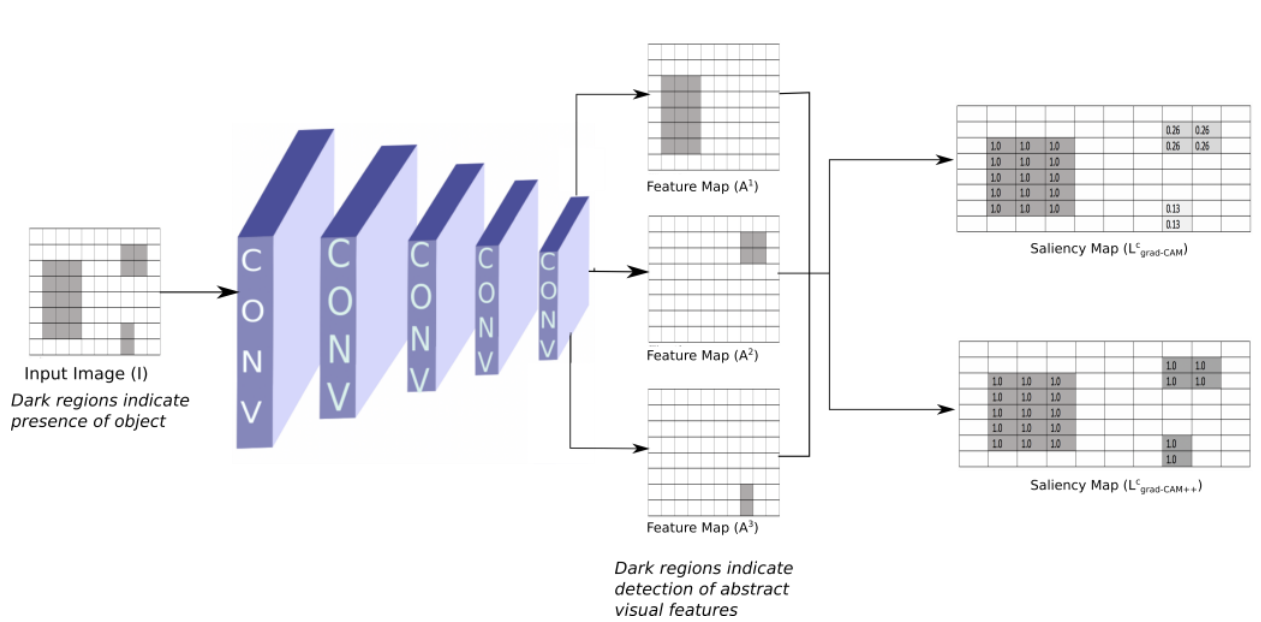
\includegraphics[width=15cm ]{fig/ch2/gradcampp1.png}
	\bicaption[\xiaosi 一个假设性的例子说明Grad-CAM++的优势]{\wuhao 一个假设性的例子说明Grad-CAM++的优势}{\wuhao A hypothetical example elucidating the intuition behind Grad-CAM++}
	\label{fig:gradcampp1}
\end{figure}


Grad-CAM++为了解决这一现象则没有直接将梯度矩阵直接全剧平均池化取平均值来作为特征图权重,而且为梯度矩阵上每一个元素赋予了一个权重,之后将梯度矩阵上的元素值全部相加取和作为特征图权重。具体的权重表示公式如下:
\begin{equation}
	w_{k}^{c}=\sum_{i} \sum_{j} \alpha_{i j}^{k c} \cdot \operatorname{ReLU}\left(\frac{\partial Y^{c}}{\partial A_{i j}^{k}}\right)  
	\label{eq:gradcampp_wkc}
\end{equation}
式\ref{eq:gradcampp_wkc}中$Y^{c}$即和章节\ref{sub:gradcam}$中\mathcal{F}_c(I)$含义一致,均表示输入图片进入模型中,模型输出的关于类别索引$c$的分数。$i$和$j$表示特征图中的$A^{k}$的行列迭代器。式\ref{eq:gradcampp_wkc}中$\alpha_{i j}^{k c}$的具体计算方式如下:
\begin{equation}
	\alpha_{i j}^{k c}=\frac{\frac{\partial^{2} Y^{c}}{\left(\partial A_{ij}^{k}\right)^{2}}}{2 \frac{\partial^{2} Y^{c}}{\left(\partial A_{i j}^{k}\right)^{2}}+\sum_{a} \sum_{b} A_{a b}^{k}\frac{\partial^{3} Y^{c}}{\left(\partial A_{i j}^{k}\right)^{3}}}
	\label{eq:gradcampp_akc}
\end{equation}
\begin{figure}[h]
	\centering 
	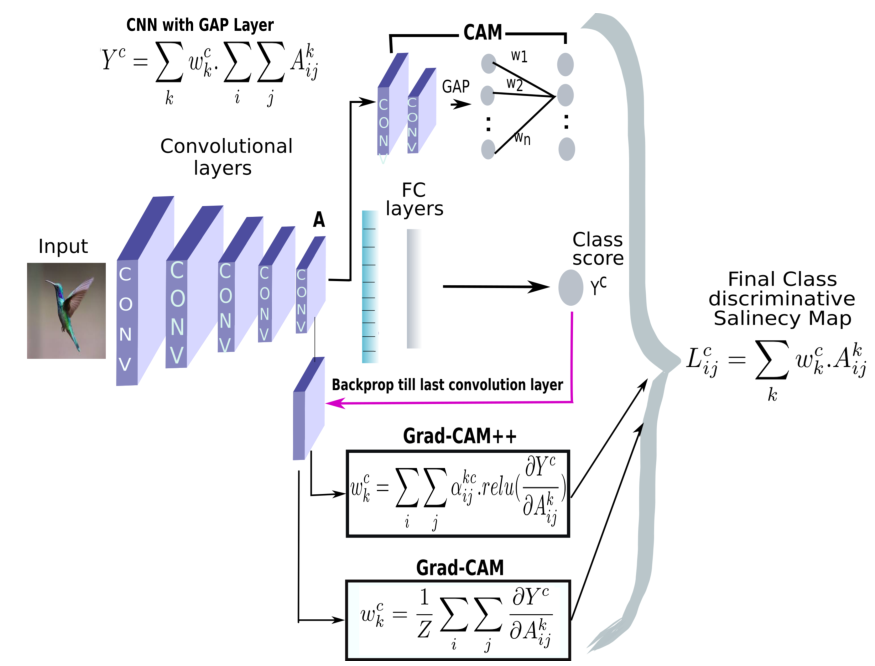
\includegraphics[width=15cm]{fig/ch2/gradcampp2.png}
	\bicaption[\xiaosi CAM, Grad-CAM, Grad-CAM++的各自计算方式]{\wuhao CAM, Grad-CAM, Grad-CAM++的各自计算方式}{\wuhao Respective calculations for CAM, Grad-CAM, Grad-CAM++}
	\label{fig:gradcampp2}
\end{figure}
将式\ref{eq:gradcampp_akc}和式\ref{eq:gradcampp_wkc}结合即可得到如下完整的权重计算公式:
\begin{equation}
	w_{k}^{c}=\sum_{i} \sum_{j}\left[\frac{\frac{\partial^{2} Y^{c}}{\left(\partial A_{i j}^{k}\right)^{2}}}{2 \frac{\partial^{2} Y^{c}}{\left(\partial A_{i j}^{k}\right)^{2}}+\sum_{a} \sum_{b} A_{a b}^{k}\frac{\partial^{3} Y^{c}}{\left(\partial A_{i j}^{k}\right)^{3}}}\right] \cdot \operatorname{ReLU}\left(\frac{\partial Y^{c}}{\partial A_{i j}^{k}}\right)
\end{equation}
得到权重后,将权重$w_{k}^{c}$和其对应的特征图$A^k$相乘,然后所有特征图线性相加即可得到Grad-CAM++生成的最终显著图。计算过程和式\ref{eq:gradcam}一致。图\ref{fig:gradcampp2}中展示了CAM、Grad-CAM、Grad-CAM++的权重计算方式异同。


\subsection{Score-CAM}
Grad-CAM和Grad-CAM++都依赖反向传播的梯度作为权重,但是这种基于梯度的方法也有缺点,若激活函数是Sigmoid函数或者ReLU函数,则会分别带来梯度饱和以及梯度消失的问题\textsuperscript{\cite{simonyan2014visualising}},反映到显著图上就是会导致噪声问题。此外依靠梯度作为权重也存在不可靠的问题,如图\ref{fig:scorecam1}所示,在这幅图中(2)(3)(4)分别是对应的特征图上采样后叠加到原图上,其中没有遮盖的部分表示该特征图在原图上较为关注的特征区域,将(2)(3)(4)通过图像分类模型,得到对应类别的得分分别是 0.003,0.999,0.997。从结果上看,(3)(4)的特征图关注的区域对于该类别是比较重要的。然而在生成Grad-CAM的显著图时,这三者计算出的权重分别是0.035,0.027,0.021。反而是对于结果影响很小的(2)的特征图权重更高。这就显示出了基于梯度的类激活映射方法的不足。


\begin{figure}[h]
	\centering 
	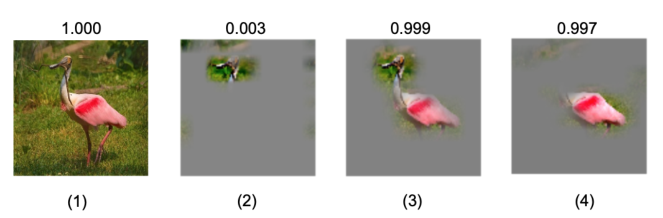
\includegraphics[width=15cm]{fig/ch2/scorecam1.png}
	\bicaption[\xiaosi 特征图扰动示例]{\wuhao 特征图扰动示例}{\wuhao Example of feature map perturbation}
	\label{fig:scorecam1}
\end{figure}

因此Score-CAM不依赖于梯度来获得特征图线性加权的权重,而是通过每张特征图在目标类上的前向传播的概率分数来获得每张特征图的权重。下面通过具体的定义来说明Score-CAM的计算方式。当输入图片为$I \in \mathbb{R}^{3\times H \times W}$时,图像分类模型为$\mathcal{F}$时,经过前向传播从指定卷积层$l$提取的第$k$个通道的特征图为$A^k_l$,那么该特征图对于指定类别$c$的概率分数$\mathcal{F}_c(I)$的贡献程度,即$A^k_l$权重$C(A^k_l)$可以由以下式子计算得出:
\begin{equation}
	C(A^k_l)=\mathcal{F}_c(I \circ H(^k_l))-\mathcal{F}_c(I_b)
	\label{eq:scorecam_C}
\end{equation}
式子\ref{eq:scorecam_C}中,$I_b$表示一张基准图像,该图像要求在类别索引$c$上的概率值尽可能的小,即$\mathcal{F}_c(I_b)$的值趋近于0,在算法实际实施的过程当中,该基准图片$I_b$一般是值均为0的全黑图像。$\circ$表示哈达玛积运算,即运算符两边的矩阵对应位置元素相乘,$H(^k_l)$是$A^k_l$上采样后的图片。其计算式子如下所示:
\begin{equation}
	H(^k_l)=s(U\!p(A^k_l))
	\label{eq:scorecam_H}
\end{equation}
式\ref{eq:scorecam_H}中,$U\!p$表示上采样运算,此处是将特征图其$A^k_l$上采样至原始输入图片尺寸。$s$表示对图片进行归一化运算,将图片中的所有像素值控制在$[0,1]$。最后可以得到Score-CAM的显著图计算式子:
\begin{equation}
	L_{\text {Score-CAM }}^{c}=\operatorname{ReLU}\left(\sum_{k} \alpha_{k}^{c} A_{l}^{k}\right)
	\label{eq:scorecam_L}
\end{equation}
式\ref{eq:scorecam_L}中,权值$\alpha_{k}^{c}$即表示$C(A^k_l)$。Score-CAM和Grad-CAM,Grad-CAM++最大的不同就是它创新性的利用特征图作为扰动输入图片的掩膜,以网络模型关于指定类别的概率分数来作为每张特征图的权重。


\subsection{LRP}
LRP全称为Layer-wise relevance propagation,意思是层间相关性传播,是深度学习中用于理解和解释神经网络决策的一种技术。LRP的主要思想是通过赋予输出结果一个相关性的分数,然后定义反向传播规则,将该相关分数逐层向后传播,通过计算给每层的每个神经元赋予一个相关性分数来表示它对输出结果的贡献程度,传播回输入层即可得到输入图片中每个像素的相关性分数,分数值的大小表示该像素与最终决策结果的相关性程度,也即贡献程度。利用获得的输入图片的每个像素的相关性分数也可以生成显著图。在传播过程中每层网络的神经元的相关性分数总和是一致的。通过这样做,LRP有助于揭示每个输入特征对最终决策的贡献,为神经网络的内部运作提供宝贵的见解。LPR的主要思想遵循以下公式:
\begin{equation}
	f(x)\approx \sum_{d=1}^{V} R_d
	\label{eq:lrp_fx}
\end{equation}
式\ref{eq:lrp_fx}中$f(x)$ 表示输入图片是$x$的情况下,其中某一个特定类别在图片$x$中的存在概率。$R_d$ 表示图片中单一像素点对该类别的相关性分数,可以看作是贡献值。图\ref{fig:lrp1}大体展示了这种分解思想。图像$x$被转换为一串特征向量,并应用分类器将图像归入给定类别,如“猫”或 “无猫”,该图中将“猫”的分类结果概率分数作为总的相关性分数反向传播至输入图片中的每个像素,最终可以得到可视化单个像素对预测的贡献。
\begin{figure}[h]
	\centering 
	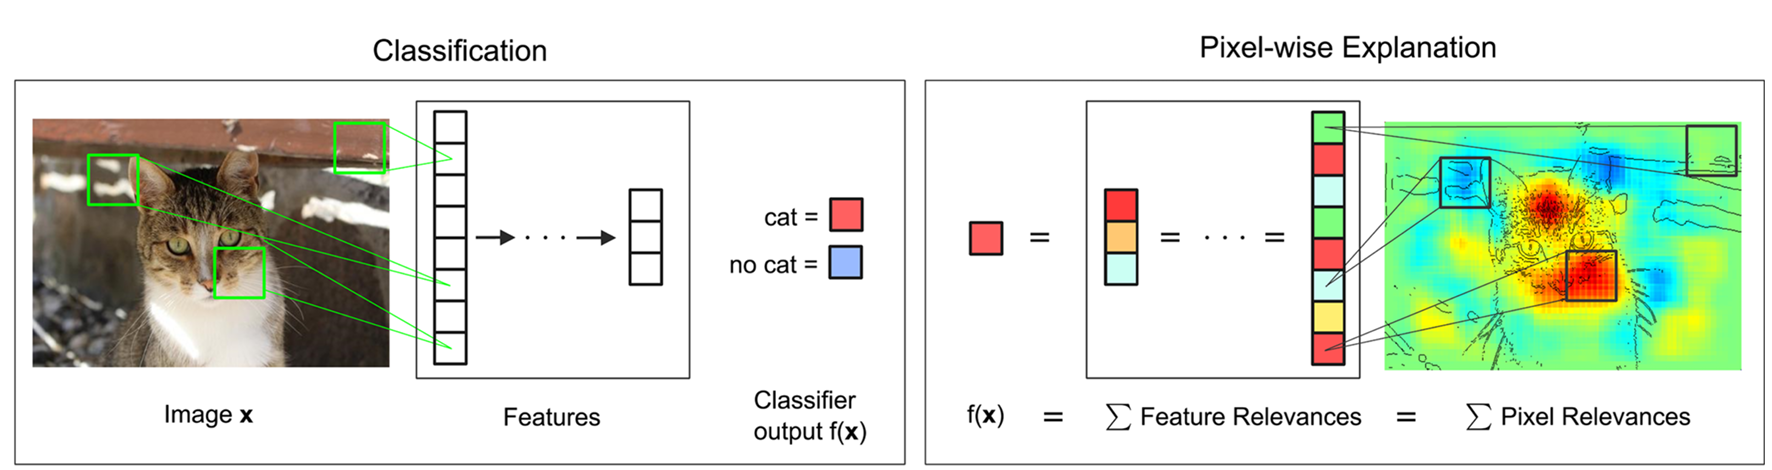
\includegraphics[width=15cm]{fig/ch2/lrp1.png}
	\bicaption[\xiaosi 像素相关性分解过程可视化]{\wuhao 像素相关性分解过程可视化}{\wuhao Visualization of the pixel relevance decomposition process}
	\label{fig:lrp1}
\end{figure}

下面结合公式推导详细说明LRP的计算过程。对于图像分类神经网络关于某个类别的输出$f(x)$有以下规则,每层的所有神经元的相关性分数是相等的。
\begin{equation}
	f(x)=\ldots=\sum_{d \in l+1} R_{d}^{l+1}=\sum_{d \in l} R_{d}^{l}=\ldots=\sum_{d} R_{d}^{1}
	\label{eq:lrp_fx2}
\end{equation}
式\ref{eq:lrp_fx2}中$l$表示神经网络的某一层,$l$越大越靠近输出层。

对于普通的多层神经网络,有如图\ref{fig:lrp2}所示的计算过程。其中:
\begin{equation}
	z_{ij}=x_iw_{ij}
	\label{eq:lrp_zij}
\end{equation}
\begin{equation}
	z_{j}=\sum_i z_{ij}+b_j
	\label{eq:lrp_zj}
\end{equation}
\begin{equation}
	x_j=g(z_{j})
	\label{eq:lrp_xj}
\end{equation}

对于式\ref{eq:lrp_zij},神经元$i$乘以其和神经元$j$之间的权重$w_{ij}$得到中间计算结果$z_{ij}$。而式\ref{eq:lrp_zj}的值是第$i$层所有神经元和权重$w _{ij}$相乘后得到的$z_{ij}$的和加上偏置项$b_j$得到的。最后$z_j$经过激活函数$g$得到第$j$层某个神经元的值$x_j$。这三个式子的意思可以总结成所有上层神经元到下层的某个神经元$j$的值,也可以理解成贡献,决定了下层神经元$j$的中间值$z_j$,只不过最后要加上偏置项和经过激活函数。

\begin{figure}[h]
	\centering 
	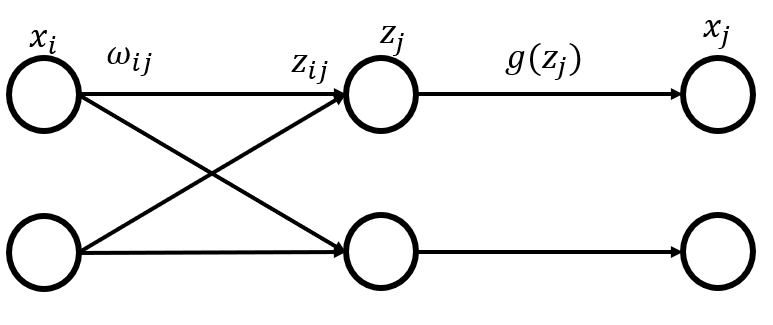
\includegraphics[width=15cm]{fig/ch2/lrp2.png}
	\bicaption[\xiaosi 多层神经网络前向传播计算示例]{\wuhao 多层神经网络前向传播计算示例}{\wuhao Example of a multilayer neural network forward propagation calculation}
	\label{fig:lrp2}
\end{figure}



从以上前向传播的示例过程中可以推导出LRP相关性传播的基本过程,如图\ref{fig:lrp3}所示,左半部分是前向传播的过程,右半部分是LRP的相关性反向传播的过程,其中$R_i^{(l)}$表示第$l$层神经元$i$的相关性分数,$R_{i\leftrightarrow j}^{(l,l+1)}$表示$l+1$层的某个神经元$j$的相关性等于$l+1$层的神经元$j$给$l$层所有神经元的相关性之和。下面结合图\ref{fig:lrp4}进行详细说明。
\begin{figure}[h]
	\centering 
	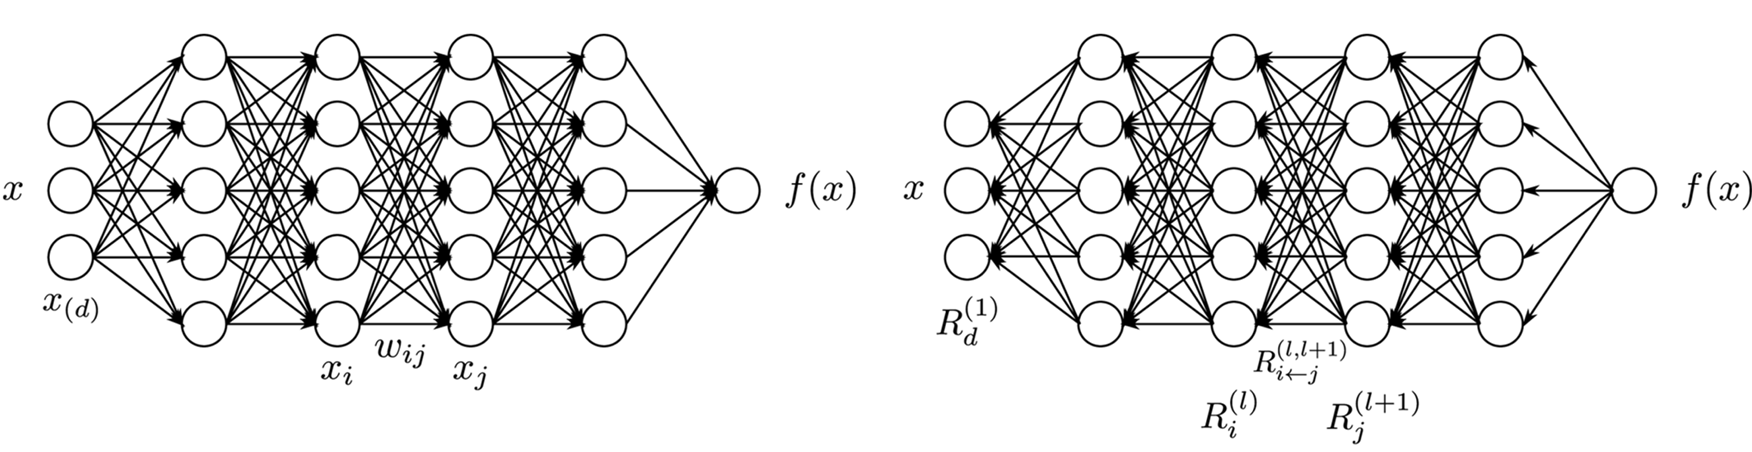
\includegraphics[width=15cm]{fig/ch2/lrp3.png}
	\bicaption[\xiaosi 多层神经网络下前向传播和层间相关性传播过程]{\wuhao 多层神经网络下前向传播和层间相关性传播过程}{\wuhao Forward propagation and LRP processes under multilayer neural networks}
	\label{fig:lrp3}
\end{figure}

\begin{figure}[h]
	\centering 
	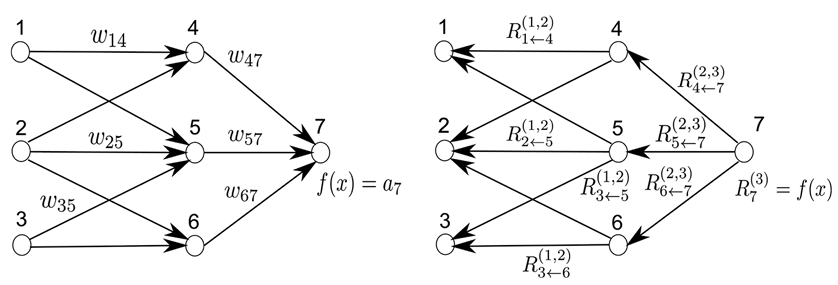
\includegraphics[width=15cm]{fig/ch2/lrp4.png}
	\bicaption[\xiaosi 层间相关性传播分配相关性分数的例子]{\wuhao 层间相关性传播分配相关性分数的例子}{\wuhao Example of LRP assigning relevance scores}
	\label{fig:lrp4}
\end{figure}
在图\ref{fig:lrp4}中的右半部分,第3层的7号神经元的相关性分数$R_{7}^{(3)}$相关性反向传播时是按照如下式子分配的:
\begin{equation}
	R_{7}^{(3)}=R_{4 \leftarrow 7}^{(2,3)}+R_{5 \leftarrow 7}^{(2,3)}+R_{6 \leftarrow 7}^{(2,3)}
\end{equation}
其中$R_{4 \leftarrow 7}^{(2,3)}$、$R_{5 \leftarrow 7}^{(2,3)}$和$R_{6 \leftarrow 7}^{(2,3)}$的值,也就是7号神经元分配给第二层的4,5和6号神经元的相关性分数在神经网络是线性的情况下(没有激活函数)可以结合公式\ref{eq:lrp_zij}进行计算,具体计算公式如下:
\begin{equation}
	R_{i \leftarrow j}^{(l, l+1)}=\frac{z_{i j}}{\sum_{i} z_{i j}} R_{j}^{(l+1)}
	\label{eq:lrp_Rij}
\end{equation}
式\ref{eq:lrp_Rij}的含义就是就是下层的神经元$j$的分配给上层神经元$j$相关性分数是$j$的总相关性分数乘以神经元$i$输出给$j$的值占$j$收到上层所有值的比。

但是在实际应用当中,神经网络会存在激活函数和偏置,式\ref{eq:lrp_Rij}无法完美应用。考虑到激活函数是双曲正切$Tanh(x)$和$ReLU$函数的情况,可以用以下公式取近似值:
\begin{equation}
	R_{i \leftarrow j}^{(l, l+1)}=\frac{z_{i j}}{z_{j}} R_{j}^{(l+1)}
\end{equation}
其他激活函数情况可以使用如下式子计算:
\begin{equation}
	\sum_{i} R_{i \leftarrow j}^{(l, l+1)}=R_{j}^{(l+1)} \cdot\left(1-\frac{b_{j}}{z_{j}}\right)
\end{equation}

\subsection{Transformer attribution}
Transformer attribution是H.Chefer等人\textsuperscript{\cite{chefer2021transformer}}于近些年提出的针对基于Transformer架构的深度神经网络的可解释方法,其在图像分类神经网络上也能够生成质量较高的显著图。Transformer attribution针对Transformer的特殊结构改进了传统的LRP算法,针对相关性反向传播过程中的注意力层和残差连接的提出了特殊的LRP传播规则,同时将其应用到基于Transformer的图片分类模型中,相比之前的可视化算法,Transformer attribution得到了较为可靠的显著图结果。

下面是Transformer attribution的详细推导过程。对于LRP传播,总是遵守以下规则:
\begin{equation}
	\sum_{j} R_{j}^{(n)}=\sum_{i} R_{i}^{(n-1)}
\end{equation}
即每层的相关性分数总和总是相等的。


若用$L^{(n)}(\mathbf{X},\mathbf{Y})$表示层对两个张量$\mathbf{X}$和$\mathbf{Y}$的操作。通常,这两个张量是第$n$层的输入特征映射和权重。则LRP遵循通用深度泰勒分解\textsuperscript{\cite{montavon2017explaining}}的规则,具体如下表示:

\begin{equation}
	R_{j}^{(n)} =\mathcal{G}\left(\mathbf{X}, \mathbf{Y}, R^{(n-1)}\right) =\sum_{i} \mathbf{X}_{j} \frac{\partial L_{i}^{(n)}(\mathbf{X}, \mathbf{Y})}{\partial \mathbf{X}_{j}} \frac{R_{i}^{(n-1)}}{L_{i}^{(n)}(\mathbf{X}, \mathbf{Y})}
	\label{eq:trans_Rnj1}
\end{equation}
对于激活函数是ReLU的情况,第$n$层的第$j$个神经元的相关性分数可以如下计算:
\begin{equation}
	R_{j}^{(n)}=\mathcal{G}\left(x^{+}, w^{+}, R^{(n-1)}\right)=\sum_{i} \frac{x_{j}^{+} w_{j i}^{+}}{\sum_{j^{\prime}} x_{j^{\prime}}^{+} w_{j^{\prime} i}^{+}} R_{i}^{(n-1)}
	\label{eq:trans_Rnj2}
\end{equation}
式\ref{eq:trans_Rnj1}和式\ref{eq:trans_Rnj2}中,$j$是和第$n$层的神经元对应的,$i$和第$n-1$层的神经元对应,$j^{\prime}$是第$n$层神经元的取和过程中的迭代计数符号。加号表示只保留正值,计算方式为$max(0,x)$。但是Transformer使用的是GELU函数,有正值也有负值同时也是非线性函数。其相关性分数计算方式如下:
\begin{equation}
	R_{j}^{(n)}  =\mathcal{G}_{q}\left(x, w, q, R^{(n-1)}\right) \\
	 =\sum_{\{i \mid(i, j) \in q\}} \frac{x_{j} w_{j i}}{\sum_{\{j^{\prime} \mid\left(j^{\prime}, i\right) \in q\}} x_{j^{\prime}} w_{j^{\prime} i}} R_{i}^{(n-1)}
\end{equation}
其中$q=\left\{(i, j) \mid x_{j} w_{j i} \geq 0\right\}$,表示只考虑对输入结果有正向贡献的相关性值。

在注意力层中有两个特征图作为输入,因此要分别考虑两者的相关性计算。假设有张量$u$和$v$,那么它们各自的相关性分数计算表示如下:
\begin{equation}
	R_{j}^{u^{(n)}}=\mathcal{G}\left(u, v, R^{(n-1)}\right), \quad R_{k}^{v^{(n)}}=\mathcal{G}\left(v, u, R^{(n-1)}\right)
\end{equation}
同时它们满足相关性守恒的原则:
\begin{equation}
	\sum_j R_{j}^{u^{(n)}}+ \sum_k R_{k}^{v^{(n)}}=\sum_i R_{i}^{(n-1)}
	\label{eq:trans_sum}
\end{equation}
式\ref{eq:trans_sum}中$u$和$v$两个向量做加法操作(对应跳跃连接的情况)时满足上述相关性原则,但是当两者作乘法时(对应注意力层矩阵乘法的情况)则不适用。因此为了解决由于矩阵乘法导致的在注意机制下相关性不守恒以及跳跃连接时存在的数值膨胀问题,Transformer attribution使用如下公式\ref{eq:trans_Ru}和式\ref{eq:trans_Rv}分别计算$u$和$v$的相关性:

\begin{equation}
	\bar{R}_{j}^{u^{(n)}}=R_{j}^{u^{(n)}} \frac{\left|\sum_{j} R_{j}^{u^{(n)}}\right|}{\left|\sum_{j} R_{j}^{u^{(n)}}\right|+\left|\sum_{k} R_{k}^{v^{(n)}}\right|} \cdot \frac{\sum_{i} R_{i}^{(n-1)}}{\sum_{j} R_{j}^{u^{(n)}}}
	\label{eq:trans_Ru}
\end{equation}

\begin{equation}
	\bar{R}_{k}^{v^{(n)}}=R_{k}^{v^{(n)}} \frac{\left|\sum_{k} R_{k}^{v^{(n)}}\right|}{\left|\sum_{j} R_{j}^{u^{(n)}}\right|+\left|\sum_{k} R_{k}^{v^{(n)}}\right|} \cdot \frac{\sum_{i} R_{i}^{(n-1)}}{\sum_{k} R_{k}^{v^{(n)}}}
	\label{eq:trans_Rv}
\end{equation}

经过规范化的计算公式在各网络层满足$\sum_{i} R_{i}^{(n)}=1$,且完全满足各层相关性守恒的原则即式\ref{eq:trans_conservation}所表示的含义。此外,每个张量的相关性和也遵循式\ref{eq:trans_restrict}的规则限制,该规则意思即第n层的每个张量的相关性和都不超过第n-1层所有相关性和。
\begin{equation}
	\sum_{j} \bar{R}_{j}^{u^{(n)}}+ \sum_{k} \bar{R}_{k}^{v^{(n)}} =\sum_{i} R_{i}^{(n-1)}
	\label{eq:trans_conservation}
\end{equation}

\begin{equation}
	0 \leq \sum_{j} \bar{R}_{j}^{u^{(n)}}, \sum_{k} \bar{R}_{k}^{v^{(n)}} \leq \sum_{i} R_{i}^{(n-1)}
	\label{eq:trans_restrict}
\end{equation}

假设$M$是一个包含$B$个模块的基于Transformer的模型,每个模块包含自注意力层、跳跃连接(残差连接)、线性层和规范化层。该模型将输入转为$s$个token,并且每个token的尺寸大小是$d$,且包含一个特殊的token用来分类,该token记为[CLS]。模型$M$输出一个长度为$C$的分类概率向量$y$,使用分类token计算。自注意模块作用于嵌入维数$d$的一个子空间$d_h$上,$h$为“头”的个数,令$d_h=d$。自注意模块定义如下:
\begin{equation}
	\mathbf{A}^{(b)}=\operatorname{softmax}\left(\frac{\mathbf{Q}^{(b)} \cdot \mathbf{K}^{(b)^{T}}}{\sqrt{d_{h}}}\right) 
	\label{eq:trans_ab}
\end{equation}
\begin{equation}
	\mathbf{O}^{(b)}=\mathbf{A}^{(b)} \cdot \mathbf{V}^{(b)}
	\label{eq:trans_ob}
\end{equation}
式\ref{eq:trans_ob}和\ref{eq:trans_ab}中,运算符$(\cdot)$表示矩阵乘法,$\mathbf{O}^{(b)} \in \mathbb{R}^{h\times s \times d_h}$是注意力模块$b$的输出。$\mathbf{Q}^{(b)},\mathbf{K}^{(b)},\mathbf{V}^{(b)} \in \mathbb{R}^{h\times s \times d_h}$分别表示Query,Key,Value向量。$\mathbf{A}^{(b)} \in \mathbb{R}^{h\times s \times s}$是模块$b$的注意力图,其中第$i$行表示输入中每个token相对于第$i$个token的相关性系数,由于式\ref{eq:trans_ab}中的归一化运算(softmax),$\mathbf{A}^{(b)}$中每个注意力头的每一行的值的和为1。

按照相关性传播和梯度传播的过程,每个注意力图$\mathbf{V}^{(b)}$对于目标类别$c$都有其梯度矩阵$\nabla \mathbf{A}^{(b)}$和相关性矩阵$R^{(n_b)}$,其中$n_b$是模块$b$中对应于式\ref{eq:trans_ab}中softmax操作的那一层。

经过上述介绍,Transfomer attribution的输出$\mathbf{C} \in \mathbb{R}^{h\times s \times s}$则由以下式子定义并计算得出:

\begin{equation}
	\bar{\mathbf{A}}^{(b)} = I + \mathbb{E}_h(\nabla \mathbf{A}^{(b)} \circ R^{(n_b)})^+
	\label{eq:trans_ab_bar}
\end{equation}

\begin{equation}
	 \mathbf{C} = \bar{\mathbf{A}}^{(1)} \cdot \bar{\mathbf{A}}^{(2)} \cdot ... \cdot \bar{\mathbf{A}}^{(B)}
	\label{eq:trans_c}
\end{equation}
式\ref{eq:trans_ab_bar}表示单个模块输出计算。运算符$\circ$表示哈达玛积运算,$\mathbb{E}_h$表示取所有注意力头上的一个平均值,$+$表示只考虑正相关性的值,即对结果有正向贡献的值,并且考虑到跳跃连接的影响,为了防止计算结果出现全0,最后加上单位矩阵。

如式\ref{eq:trans_c}所示,Transfomer attribution的最终解释输出是一个$s\times s$的矩阵$\mathbf{C}$,$s$表示经过输入到Transformer Encoder中的序列长度。$\mathbf{C}$中的每行对应于一个token对于其他token的相关性权重序列。由于是考虑基于Transformer的图像分类神经网络,因此只用考虑封装了分类信息的[CLS]的token的相关性序列,即$\mathbf{C}_{[CLS]} \in \mathbb{R}^s$对应于$\mathbf{C}$中的关于[CLS]token的那一行,因此该行中每个分数即是对每个输入token对输出分类的相关性分数。

不考虑其他特殊token,比如[CLS]等,在实际的基于Transformer的图像分类神经网络ViT\textsuperscript{\cite{dosovitskiy2020image}}中,每一个输入token表示一个图像块,为了获得最终的显著图,则需要将获得相关性序列$\mathbf{C}_{[CLS]} \in \mathbb{R}^s$进行重新调整,调整为尺寸为$\sqrt{s-1}\times \sqrt{s-1}$的原始显著图,由于$s-1$的数值一般为图像块的个数,因此原始显著图分辨率较低,需要将其通过插值进行上采样为最终显著图。下图\ref{fig:trans1}展示了Transformer attribution计算过程,对应于式\ref{eq:trans_ab_bar}和式\ref{eq:trans_c}。
\begin{figure}[h]
	\centering 
	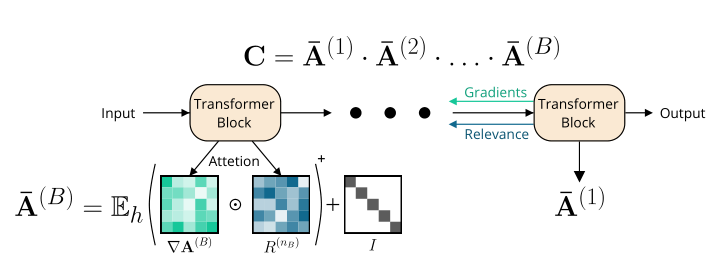
\includegraphics[width=15cm]{fig/ch2/trans1.png}
	\bicaption[\xiaosi Transformer attribution 计算过程]{\wuhao Transformer attribution 计算过程}{\wuhao Transformer attribution calculation procedure}
	\label{fig:trans1}
\end{figure}

\section{本章小结}
本章首先简要介绍了卷积神经网络和Transformer架构的基础原理,它们也是当前图像分类神经网络的两种主要基础架构。然后本章重点介绍了当前5种比较著名的显著图解释方法的背后原理和显著图生成的计算过程,这5种方法分别是Grad-CAM,Grad-CAM++,Score-CAM,LRP和Transformer a ttribution。这5种显著图解释方法也是第3章和第4章实验对比的其中一些方法。






% 第3章


\chapter{基于输入图片多尺寸放大的卷积神经网络显著图解释方法}
\thispagestyle{others}
\pagestyle{others}
\xiaosi

\section{本章引言}



\section{问题描述和研究思路}
当前大多数基于类激活映射的显著图解释方法诸如CAM、Grad-CAM、Grad-CAM++、XGrad-CAM、Score-CAM等都存在一个共有问题,即最终生成的显著图的分辨率较低,这导致其只能在显著图中呈现一个模糊的解释效果,无法聚焦更加精细的特征。究其原因是这些基于类激活映射的方法一般提取的都是卷积神经网络的最后一层卷积层的输出作为特征图的来源,因该层包含较为丰富的类别特征信息,之后通过各种加权方法组合这些特征图来得到最终的显著图。因为卷积神经网络的结构特性,其最后一层卷积层的会输出多个通道的低分辨率特征图,因此无论如何组合这些特征图,最终得到的也只是一张分辨率和最后一层的卷积层输出的单一通道的特征图相当的初级显著图。当然一般情况下为了得到显著图和原始输入图片的特征对应关系,都会将这张原始输入图片进行分辨率层面的放大,使用的一般也是双线性插值算法,但这并不意味着原始显著图的有效信息的增多。

这里以VGG19这个基于卷积神经网络的图片分类模型举例,若输入图片的尺寸是3$\times$224$\times$224,其中3表示RGB颜色通道,224$\times$224表示图片分辨率,那么该模型最后一层卷积层的输出的特征图尺寸是512$\times$14$\times$14,其中数字512是通道数量,14$\times$14是特征图的分辨率。若我们使用双线性插值函数$\phi(s,H,W)$将原始显著图分辨率提升到224$\times$224,那么意味着我们插入了额外99.9\%的信息,而最终的显著图中的这些额外的像素信息并不能反映图片分类模型对原始输入图片的对应像素的感兴趣程度。即便有部分文献\textsuperscript{\cite{adebayo2018sanity}\cite{selvaraju2017grad}}试图改进这种插值函数,但是它们仍然引入了外部不相关的信息。

因此为了解决上述的问题,本文从特征图的提取这一关键点着手。考虑到若使用原始输入图片,那么卷积神经网络最后一层卷积层输出的单一特征图分辨率较低且包含的特征信息有限,因此本文提出基于输入图片多尺寸放大的卷积神经网络显著图解释方法,其核心就是将输入图片进行逐级多尺寸的双线性插值放大,例如将输入图片放大至334$\times$334、434$\times$434、534$\times$534等分辨率,这时能得到一组分辨率不同的输入图片,接着将这组输入图片分别送入基于卷积神经网络的图像分类模型中,再从其最后一层卷积层中分别提取特征图和梯度矩阵数据,基于卷积神经网络的采样特性,可以得到不同分辨率的特征图,更高分辨率的输入图片即对应更高分辨率的特征图,也即拥有更丰富的特征信息。因此若将这些特征图的信息进行融合即能得到分辨率更高的掩膜,再用这些更高分辨率的掩膜对原始输入图片进行扰动,即可得到相应的掩膜权重,用权重和高分辨率掩膜进行融合即能得到包含更多特征信息并且分辨率更高的显著图。
\section{基于输入图片多尺寸放大的卷积神经网络显著图解释方法}
本章提出基于基于输入图片多尺寸放大的卷积神经网络显著图解释方法来解决目前可视化算法结果分辨率低、无法给出更详细目标特征的问题。为了方便本章后文的描述,本文对该方法的简称是MSG-CAM(Multi-Scale inputs of Group-
CAM)。MSG-CAM的算法流程描述参见算法\ref{alg:1},算法流程图参见图\ref{fig:msg_pipeline}。

\begin{figure}[h]
	\centering 
	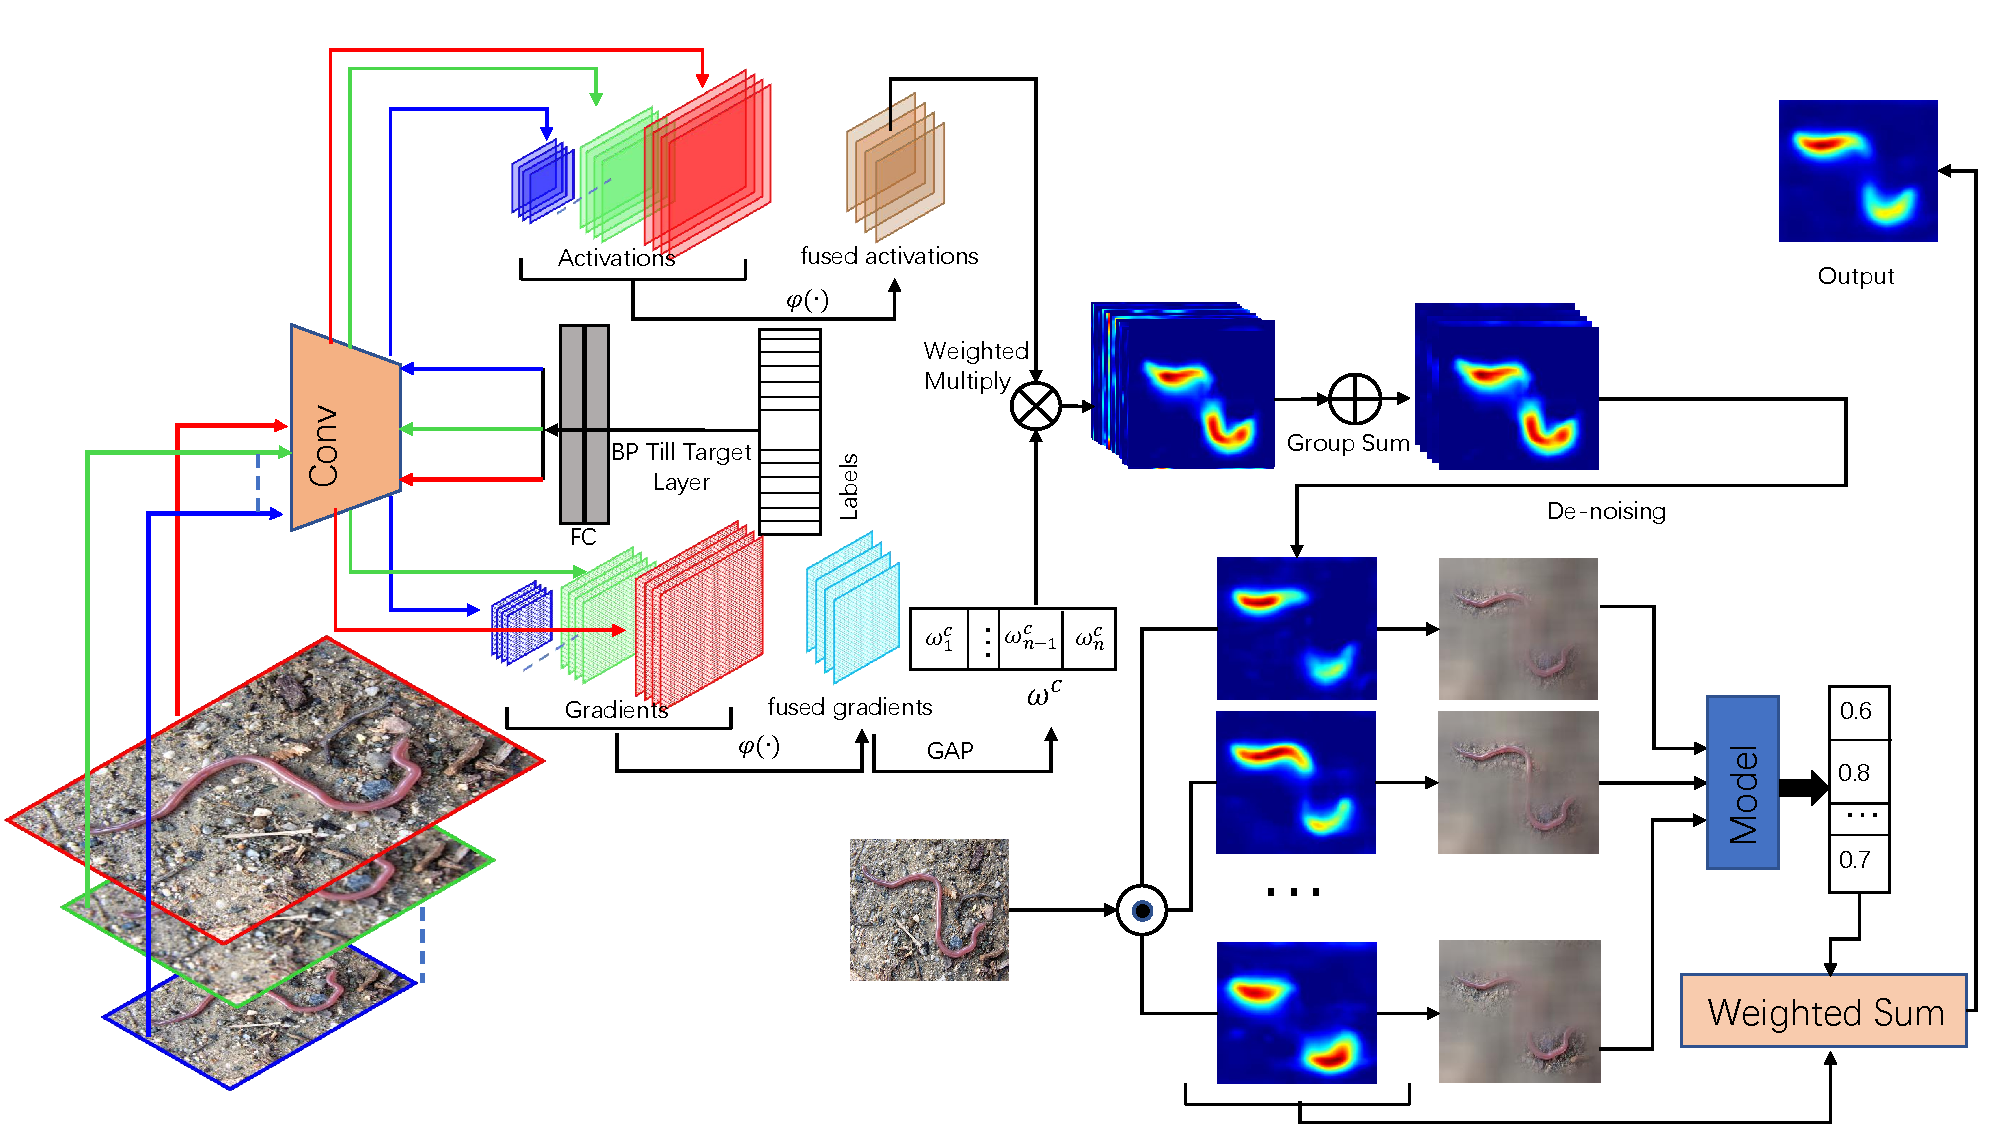
\includegraphics[width=15cm]{fig/ch3/msg_pipeline.pdf}
	\bicaption[\xiaosi MSG-CAM算法流程示意图]{\wuhao MSG-CAM算法流程示意图}{\wuhao Pipeline of MSG-CAM}
	\label{fig:msg_pipeline}
\end{figure}

 \begin{algorithm}
	\caption{MSG-CAM}
	\label{alg:1}
	\renewcommand{\algorithmicrequire}{\textbf{输入:}}
	\renewcommand{\algorithmicensure}{\textbf{输出:}}
	\begin{algorithmic}[1]
		\REQUIRE 基于卷积神经网络的图像分类模型 $\mathcal{F} $ ,原始输入图片 $I_0 \in \mathbb{R}^{3\times H_0 \times W_0}$ ,上采样分辨率上限 $\zeta_{max}=(H_{max},W_{max})$ ,卷积层 $l$ ,最大迭代次数 $N$ ,类别 $c$ ,每个分组中掩膜数量$B$, 高斯模糊参数: $kernel\_size,sigma$, interpolation function $\varphi(.)$
		\ENSURE 显著图 $L_{MSG-CAM}\in \mathbb{R}^{3\times H_0 \times W_0}$
		\STATE 初始化 $L_{MSG-CAM} \leftarrow 0$ , $\mathcal{A}_0 \leftarrow 0$ , $\mathcal{G}_0 \leftarrow 0$ , $r \leftarrow 0$ , $t_{max}\leftarrow 0$ , $t_m\leftarrow 0$ , $kernel\_size=51,sigma=50$ ,基准图片 $I^{\prime}_0=guassian\_blur2d(I_0,kernel\_size,sigma)$ , $c=\mathcal{F}(I_0)$
		\WHILE{$t\leq N$}
		\STATE $t\leftarrow t+1$
		\STATE $\zeta_t\leftarrow \zeta_0 +\lfloor\frac{\zeta_{max}}{N}\rfloor(t-1)$
		\STATE $I_t\leftarrow \varphi(I_0,\zeta_t)$
		\IF{$\mathcal{F}(I_t) \rightarrow c$}
		\STATE $t_{max}\leftarrow t_{max}+1$
		\STATE $\overset{*}{\boldsymbol{A}_t}\leftarrow \mathcal{A}(I_t,l)$
		\STATE $\overset{*}{\boldsymbol{G}_t}\leftarrow \nabla\mathcal{J}(l,c)$
		\STATE $\mathcal{A}_t \leftarrow \mathcal{A}_{t-1}+\varphi(\overset{*}{\boldsymbol{A}_t},\zeta_0)$
		\STATE $\mathcal{G}_t \leftarrow \mathcal{G}_{t-1}+\varphi(\overset{*}{\boldsymbol{G}_t},\zeta_0)$
		\ENDIF
		\ENDWHILE
		\STATE $\overline{\bm{A}}\leftarrow \mathcal{A}_t/t_{max}$
		\STATE $\overline{\bm{G}}\leftarrow \mathcal{G}_t/t_{max}$
		\STATE $\overline{\bm{W}}\leftarrow \frac{1}{m\times n}\sum_{i=i}^{m}\sum_{j=1}^{n}\overline{\bm{G}}$
		\STATE $\boldsymbol{M}=\overline{\bm{A}}\cdot\overline{\bm{W}}$
		\STATE $K\leftarrow$ $\boldsymbol{M}$的通道数量;
		\STATE $g\leftarrow$ 每个分组中掩膜数量;
		\WHILE{$r<B$}
		\STATE 在组内生成单一的掩膜\\ $M_r=ReLU(\sum_{k=r\times g}^{(r+1)\times g-1}M^k)$
		\STATE 初始化 $M^{\prime}_r\leftarrow$ 将$M^r$进行去噪操作和归一化
		\STATE 用掩膜扰动原始输入图片\\$I_r=I_0\odot M^{\prime}_r+I^{\prime}_0\odot (1-M^{\prime}_r)$
		\STATE 计算每张掩膜的权重\\$\alpha_r=\mathcal{F}_c(I_r)-\mathcal{F}_c(I^{\prime}_0)$
		\STATE $L_{MSG-CAM}\leftarrow L_{MSG-CAM}+\alpha_r M_r$
		\STATE $r\leftarrow r+1$
		\ENDWHILE
		\RETURN $ReLU(L^c_{MSG-CAM})$
	\end{algorithmic}
\end{algorithm}
\subsection{生成高分辨率掩膜}
令原始输入图片为$I_0 \in \mathbb{R}^{3\times H_0 \times W_0}$,其中3表示RGB颜色通道数量,$H_0$和$W_0$分别原始输入图片的长和宽的像素个数,即原始输入图片的分辨率可以表示为$\zeta_0=(H_0,W_0)$。此外,我们用$\mathcal{F}$表示一个预训练好的基于卷积神经网络的图像分类模型,那么$\mathcal{F}_c(I_0)$则表示在输入图片为$I_0$的情况下,图像分类模型$\mathcal{F}$对于类别$c$的输出分数,值得注意的是,该分数是未经归一化指数函数(softmax函数)之前的分数。将原始输入图片送入图像分类模型$\mathcal{F}$,并从其最后一层卷积层$l$当中提取所有通道的特征图集合,该特征图集合表示为$\overset{*}{\boldsymbol{A}_0}$。通过获得的类别$c$的输出分数$\mathcal{F}_c(I_0)$,对该分数反向传播至最后一层卷积层特征图,则可以获得对应特征图关于类别$c$的梯度矩阵$\overset{*}{\boldsymbol{G}_0}$,计算公式如下:
\begin{equation}
\overset{*}{\boldsymbol{G}_0}=\frac{\partial \mathcal{F}_c(I_0)}{\partial \overset{*}{\boldsymbol{A}_0}}
\label{eq:g0}
\end{equation}
\ref{eq:g0}公式中,梯度矩阵集合$\overset{*}{\boldsymbol{G}_0}$一共有$K$个通道,通道数量和特征图集合$\overset{*}{\boldsymbol{A}_0}$一致,并且每个通道的梯度矩阵和特征图一一对应。 

接着将原始输入图片$I_0$经由双线性插值函数$\varphi(I_0,\zeta_t)$上采样至图片$I_t$,$t$表示第$t$次上采样结果,经由上采样后的$I_t$的分辨率可表示为$\zeta_t$,$\zeta_t$是由于原始输入图片的分辨率$\zeta_0$逐步递增得来的。为了控制计算的时间成本,考虑将$\zeta_{max}=(H_{max},W_{max})$作为上采样分辨率的上限,同时设$N$为最大迭代次数即上采样次数,那么第$t$次上采样得到的图片分辨率可由以下公式计算得出:
\begin{equation}
	\zeta_t=\zeta_0 +\lfloor\frac{\zeta_{max}}{N}\rfloor(t-1)
\end{equation}
在上述迭代过程当中,每次上采样获得的输入图片$I_t$的分辨率都不同,则将其输入到图像分类模型当中$\mathcal{F}$从最后一层卷积层提取的特征图集合$\overset{*}{\boldsymbol{A}_t}$的分辨率也不同,而且随着输入图片分辨率的提高,$\overset{*}{\boldsymbol{A}_t}$的分辨率也会相应提高,相对应的$\overset{*}{\boldsymbol{A}_t}$也能包含更多和类别$c$相关的细节特征信息。因此若将这些不同的分辨率的特征图集合进行融合则能够得到更多的特征信息。融合的方法可由以下的公式进行表示:
\begin{equation}
	\overline{\bm{A}}=\frac{1}{t_{max}}\sum_{t=0}^{t_{max}}\varphi(\overset{*}{\boldsymbol{A}_t},\zeta_0)
	\label{eq:Afuse}
\end{equation}
公式\ref{eq:Afuse}中,$t_{max}$表示最大的有效迭代次数,此处的“有效”指的是只有当图像分类模型的输出结果中概率分数最大的类别是$c$时才采用这次迭代的特征图集合$\overset{*}{\boldsymbol{A}_t}$,其他情况下均舍弃,因此不难得出$t_{max} \leq N$。同时$\varphi(\overset{*}{\boldsymbol{A}_t},\zeta_0)$表示将特征图集合$\overset{*}{\boldsymbol{A}_t}$中的每一个通道上的特征图均上采样至原始输入图片的分辨率$\zeta_0$,这样做的目的是方便将不同分辨率的特征图集合进行融合,也方便后续对原始输入图片进行扰动。

在每次迭代过程中,都会计算并提取保存图像分类模型关于类别c的输出分数$\mathcal{F}_c(I_t)$对于卷积层$l$的特征图集合$\overset{*}{\boldsymbol{A}_t}$的反向传播梯度$\overset{*}{\boldsymbol{G}_t}$,和特征图集合一样,将不同迭代过程中保存的梯度矩阵集合$\overset{*}{\boldsymbol{G}_t}$也进行融合,可以得到$\overline{\bm{A}}$分辨率尺寸一致梯度矩阵集合,融合的公式如下所示:
\begin{equation}
	\overline{\bm{G}}=\frac{1}{t_{max}}\sum_{t=0}^{t_{max}}\varphi(\overset{*}{\boldsymbol{G}_t},\zeta_0)
	\label{eq:Gfuse}
\end{equation}
同样,公式\ref{eq:Gfuse}中,同时$\varphi(\overset{*}{\boldsymbol{G}_t},\zeta_0)$表示将梯度矩阵集合$\overset{*}{\boldsymbol{G}_t}$中的每一个通道上的梯度矩阵均上采样至原始输入图片的分辨率$\zeta_0$。由于融合后的特征图集合中不仅包含类别$c$特征信息,也包含其他类别的特征信息,因此为了将类别$c$的特征信息进行凸显,其他类别的特征信息进行削弱,我们将利用融合后的梯度矩阵$\overline{\bm{G}}$,它在一定程度上反映了特征图上不同像素对类别分数$\mathcal{F}_c(I_0)$的敏感程度,或者说是重要程度\textsuperscript{\cite{selvaraju2017grad}3}。仿照Grad-CAM\textsuperscript{\cite{selvaraju2017grad}4}中的方法,我们将$\overline{\bm{G}}$中每张梯度矩阵进行全局平均池化,在每个通道上得到一个权重值,每个通道下的权重值都和$\overline{\bm{A}}$中的每个通道下的特征图一一对应,所有通道下权重值的集合的计算公式如下:
\begin{equation}
	\overline{\bm{W}}=\frac{1}{H_0\times W_0}\sum_{i=1}^{H_0}\sum_{j=1}^{W_0}\overline{\bm{G}}
	\label{eq:Wfuse}
\end{equation}
额外说明的是,融合后的特征图集合$\overline{\bm{A}}$的尺寸是$[1\times K \times H_0\times W_0]$,它对应的权重集合$\overline{\bm{W}}$的尺寸是$[1\times K \times 1\times 1]$,其中$K$就是第$l$层卷积层输出的特征图通道数量。

本小节的最后,初始掩膜集合$\boldsymbol{M}$可以通过以下公式计算得出:
\begin{equation}
	\boldsymbol{M}=	\overline{\bm{A}}\cdot\overline{\bm{W}}
\end{equation}
其中,运算符$\cdot$表示$\overline{\bm{A}}$中的每个通道下的特征图中的每个像素值都和$\overline{\boldsymbol{W}}$中对应每个权值相乘。

\subsection{掩膜优化}
$\boldsymbol{M}$是经由输入图片多尺寸上采样放大后从卷积层中提取的特征图和梯度矩阵结合而得到的,相比单一原始输入图片得到掩膜(比如Score-CAM\textsuperscript{\cite{wang2020score}2}),$\boldsymbol{M}$包含更丰富的类别特征信息,但是目前得到$\boldsymbol{M}$仍然不能直接当作掩膜来扰动输入图片,它还有两个明显的缺点。第一点是$\boldsymbol{M}$的尺寸是$[1\times K \times H_0\times W_0]$,其中$K$是卷积层$l$输出的特征图的通道数量,一般我们取最后一层卷积层作为$l$,因此$K$的值将会是数百至上千,显然这样掩膜的数量太多了,若像Score-CAM\textsuperscript{\cite{wang2020score}3}一样逐个将掩膜去扰动原始输入图片得到权值,那样将会极为耗时。第二个缺点$\boldsymbol{M}$就是使用全局平均池化后的梯度作为特征图的权重,由于ReLU函数的零梯度问题\textsuperscript{\cite{zhang2021novel}},这意味着$\boldsymbol{M}$显然会有噪声。因此,为了使$\boldsymbol{M}$成为合格的掩膜,需要让它变得更加纯净。

对于第一个缺陷,本节的解决办法是将$\boldsymbol{M}$中的$K$张掩膜平分为$B$个组,分类依据是它们的相邻关系,接着将每个组内的所有掩膜相加合并为一个掩膜,这个相加合并过程可由以下的公式计算得出:
\begin{equation}
	M_r=ReLU(\sum_{k=r\times g}^{(r+1)\times g-1}{M^k})
	\label{eq:Mr}
\end{equation}
公式\ref{eq:Mr}中$g$是每个组中的特征图的数量且 $g=K/B$,$r$的取值范围是$\{0,1,2,\dots,B-1\}$,即合并完成后一共有$B$张掩膜,$M_r$是第$r$组中合并完成后的掩膜,$M^k$是$\boldsymbol{M}$中第$k$个通道的特征图。

对于第二个缺陷,我们设计了一个去噪函数$f(m_{ij},\theta)$,该函数中$m_{ij}$是掩膜$M_r$中第$i$行第$j$列的像素值,$\theta$是一个百分比值。具体的去噪计算结果由以下公式计算得出:
\begin{equation}
	f(m_{ij},\theta)= \begin{cases}
		\ m_{ij}, & \rm if \enspace \it m_{ij}>p(M_r,\theta) ; \\
		\ 0, & \rm otherwise .\\
	\end{cases}
\label{eq:denoise}
\end{equation}
公式\ref{eq:denoise}中$p(M_r,\theta)$表示$M_r$的所有像素值从大到小处于$\theta$百分比的值,比如有100个像素值,每个像素值都是1到100中的一个整数取值且取值唯一,此时$\theta =70$,那么$p(M_r,\theta)=70$。\refeq{eq:denoise}公式的作用就是将掩膜$M_r$中百分比前$\theta$大的像素值保留,小于$p(M_r,\theta)$的像素值置为0。经过去噪操作后可以得到更加纯净的掩膜。

到目前为止,还剩下最后一个操作即可得到最终的掩膜。将$M_r$中的所有像素值进行最大最小归一化,使其像素值区间位于$[0,1]$,这样方便将掩膜直接和输入图片相乘进行扰动操作。具体计算公式如下:
\begin{equation}
	M^{\prime}_r=\frac{M_r-min(M_r)}{max(M_r)-min(M_r)}\label{e_minmax}
\end{equation}
最后,掩膜$M^{\prime}_r$有这和原始输入图片$I_0$一致的分辨率且掩膜的像素值和$I_0$中的像素值一一对应。

\subsection{生成显著图}
如果显著性方法确实识别出了对模型预测有重要意义的像素,那么这一点就应该反映在重建图像的模型输出当中\textsuperscript{\cite{kapishnikov2019xrai}}。将$M^{\prime}_r$作为掩膜来扰动原始输入图片$I_0$,其背后的原理是从原始输入图像中保留掩膜中获得的关于类别$c$的特征信息,让图像分类模型来判断保留的这部分信息的重要性,判断依据就是图像分类模型对扰动后的图片关于类别$c$的输出概率分数。但是,如果直接将掩膜和原始输入图像相乘进行扰动,那么扰动后的图像中的被掩盖区域和被凸显的区域之间的边界会过于明显锐利,从而对图像分类神经网络造成对抗效果\textsuperscript{\cite{dabkowski2017real}}。

为了遇到避免上述的问题,高斯模糊函数被引入到了接下来的改进方法中。具体方法是将扰动区域即被掩膜遮盖的区域用高斯模糊后的原始输入图片的对应区域进行替代,这样可以使得凸显的图片区域和被扰动的图片区域之间的边界更加平滑,从而像真实图片,不易让图像分类神经网络产生异常的输出。对于单一掩膜$M^{\prime}_r$,这个扰动模式可以由以下的公式计算得出:
\begin{equation}
	I_r=I_0\odot M^{\prime}_r+I^{\prime}_0\odot (1-M^{\prime}_r)
	\label{eq:Ir}
\end{equation}
公式\ref{eq:Ir}中,$I^{\prime}_0$是将原始输入图片$I_0$高斯模糊后的得到的,$I^{\prime}_0$作为一张基础图片送入图像分类模型$\mathcal{F}$当中,当然得到其关于类别$c$的输出结果$\mathcal{F}_c(I^{\prime}_0)$是一个非常低的值且趋近于0。具体的高斯模糊函数是$guassian\_blur2d(input,kernel\_size,sigma)$,在本章中,参照Group-CAM\textsuperscript{\cite{zhang2021novel}}的工作,设置高斯模糊的参数$kernel\_size=51$和$sigma=50$。 $1-M^{\prime}_r$表示$M^{\prime}_r$中每个像素值都作为减数被1相减,作用是将掩膜中关于类别$c$的特征信息进行凸显。

参考RISE\textsuperscript{\cite{petsiuk2018rise}}中的方法,每张掩膜$M_r$的权重$\alpha_r$可以由扰动后的$I_r$输入到图像分类模型$\mathcal{F}$中得到。$\mathcal{F}_c(I_r)$则是该权重,其表示模型对显著图区域中类别$c$的特征信息的感兴趣程度。具体计算公式由以下式子给出:
\begin{equation}
	\alpha_r=\mathcal{F}_c(I_r)-\mathcal{F}_c(I^{\prime}_0)
\end{equation}
最终的显著图即将所有$M_r$的权重$\alpha_r$和其本身相乘,并经过ReLU函数后得到,ReLU函数的作用是保留显著图中的正值,即模型关于类别$c$感兴趣的像素区域。具体式子如下表示:
\begin{equation}
	L_{MSG-CAM}=ReLU(\sum_{r}\alpha_r M_r)
\end{equation}
 

 
 
\section{实验与分析}

\subsection{实验硬件配置和软件环境}
下面给出本章实验的硬件配置和实验环境相关信息,具体信息见表\ref{tab:en}。

\begin{table}
	\renewcommand{\arraystretch}{1.5}
\centering
\bicaption[\xiaosi 实验环境和硬件配置]{\wuhao 实验环境和硬件配置}{\wuhao Experimental environment and hardware configuration}

	\begin{tabular}{p{4cm}p{8cm}} 
\hline
类型                  & \multicolumn{1}{c}{配置信息}      \\ 
\hline
\multirow{3}{*}{硬件} & CPU:10-core Intel$^\circledR$ Xeon$^\circledR$ W-2255 CPU                  \\
& 内存:128GB 64-bit DDR4 3700MHz  \\
& 显卡:NVIDIA RTX A5000 24GB      \\ 
\hline
\multirow{6}{*}{软件} & 操作系统:Ubuntu 20.04 LTS         \\
& Python版本:Python3.8            \\
& 深度学习框架:Pytorch 1.10.1         \\
& 计算架构:CUDA 11.4                \\
& 计算加速库:CUDNN 8.2.0             \\
& AI性能:27.8 TFLOPS              \\
\hline
\end{tabular}
\end{table}


\subsection{数据集及其预处理和实验参数说明}
在本章的实验当中,主要使用了三个数据集,下面是三个数据集的简要介绍:
1. ILSVRC 2012数据集
ILSVRC 2012(ImageNet Large Scale Visual Recognition Challenge 2012)是一个用于视觉对象识别和定位的大规模数据集和竞赛。该数据集包含超过120万张标注图片,涵盖1000个不同类别的物体和场景。ILSVRC 2012竞赛旨在推动计算机视觉领域的发展,参与者需要开发能够识别图像中物体类别的算法,并对物体进行定位。该竞赛对于深度学习和卷积神经网络等技术的发展起到了重要推动作用,成为了评估图像识别算法性能的重要基准。ILSVRC 2012数据集的发布和竞赛对于推动计算机视觉领域的发展产生了深远影响。

2. PASCAL VOC数据集
PASCAL VOC(Visual Object Classes)数据集是一个常用的计算机视觉数据集,用于目标检测、图像分割和场景分类等任务。该数据集最初由牛津大学的计算机视觉研究组创建,包含了20个常见的物体类别,如人、狗、猫、飞机等。数据集中的图像来自于自然场景和网络图像,每个图像都标注了包含的物体类别和位置信息。PASCAL VOC数据集被广泛应用于评估目标检测和图像分割算法的性能,是计算机视觉领域中的重要基准数据集之一。同时,PASCAL VOC数据集也被用于举办国际性的计算机视觉竞赛,吸引了全球的研究者和工程师参与。通过使用PASCAL VOC数据集,研究人员可以开发和评估各种视觉任务的算法,推动计算机视觉技术的发展。

3. COCO2014数据集
COCO2014数据集(Common Objects in Context)是一个用于计算机视觉任务的大型数据集,包含超过200,000张图像和相关的注释信息。这些图像涵盖了80个不同类别的物体,并且每张图像都有多个物体的标注,这使得数据集在目标检测、图像分割和物体识别等任务中非常有用。COCO2014数据集的引入为计算机视觉领域的研究和发展提供了重要的资源,成为了许多视觉任务的标准基准。研究人员和开发者可以利用该数据集进行模型训练、算法评估和性能比较,从而推动计算机视觉技术的进步。COCO2014数据集的广泛应用促进了目标检测、图像分割和物体识别等领域的发展,为相关领域的研究和应用提供了有力支持。

在本章当中插入与删除实验中使用的是ILSVRC 2012验证集,包含50000张图片,并且将该验证集中的图片尺寸调整为(3$\times$224$\times$224),其中$3$是表示RGB颜色通道数量,像素值进行归一化调整,调整后的像素值范围是[0, 1],最后使用Imagenet数据集的均值[0.229, 0.224, 0.225]和方差[0.485, 0.456, 0.406]对所有图片像素值进行标准化处理。在定点游戏实验中,使用了两个数据集,分别是PASCAL VOC数据集中的测试集,包含4952张图片,和COCO 2014数据集的验证集,包含50000张图片。用于本章实验的图像分类神经网络模型是torchvision提供的预训练模型VGG19\textsuperscript{\cite{simonyan2014very}},它是基于卷积神经网络架构的。如果没有特别说明,本章提出的方法MSG-CAM的默认设置参数是$B=32$,$\theta=70$。所有方法生成的最终显著图默认都上采样至224$\times$224的分辨率。
\subsection{定性评估}

\subsection{插入(insertion)和删除(deletion)实验}
插入(insertion)和删除(deletion)实验首次在RISE\textsuperscript{\cite{petsiuk2018rise}}实验中提出。插入实验背后所反映的原理是当我们按照显著图给出的像素重要程度优先级开始在原图的对应位置逐渐插入重要的像素直至完全插入所有像素,在此过程中记录每次插入操作时模型对指定类别给出的可能性概率分数。插入实验可以衡量显著图对像素重要性的排序是否与模型实际决策时关注的像素重要性排序一致。与之相反的是,删除实验则是按照显著图中给出的像素重要程度优先级逐渐从原输入图片中抹去对应的像素信息。和插入实验一样,删除实验也要求记录每次删除操作后模型对感兴趣类别给出的可能性分数。删除实验可以直观的呈现出缺失重要特征的像素信息后模型对感兴趣类别的置信程度下降情况。

具体而言,对于插入实验,我们将原输入图片高斯模糊化后作为画布,随后每次迭代过程中,我们按照显著图给出的像素优先级逐渐向画布中对应的位置中引入原输入图片的像素,每次迭代过程中记录模型对引入像素后的的图片关于指定类别的可能性概率分数。为了更加精确的反映显著图的像素优先级,我们每次迭代只引入约0.89\%(224$\times$2)的像素。和插入实验相对比,删除实验每次迭代将原输入图片中的像素逐渐替代为画布上的像素,直到输入图片被完全替换为画布为止。删除实验每次迭代仍然是变更约0.89\%的在原图中的像素。需

要特别说明的是,我们引入高斯模糊后的原输入图片作为画布是为了避免引入像素或者删除像素时产生过于锐利的边界,从而更加接近真实图片,避免产生对抗攻击的样本。此外,每次迭代记录的可能性分数都是经过softmax函数进行归一化后的数据。得到插入实验和删除实验每次迭代获得的分数后,我们使用概率分数随插入或者删除次数的曲线的曲线下面积(Area Under Curve)作为的作为量化指标。为了总体衡量插入实验和删除实验的优劣,我们使用总体(over-all)分数。按照上面关于插入实验和删除实验的描述,AUC(insertion)越高表明显著图越准确,同理,AUC(deletion)越低越好。因此,overall分数计算方式是AUC(insertion)-AUC(deletion)。图\ref{fig:IDCurve}展示了Grad-CAM、Score-CAM、Group-CAM和MSG-CAM为所选的4幅代表性图像生成了显著图以及相应的插入和删除曲线。对于删除曲线,更好的显著图解释方法给出的显著性图应尽可能快地下降,插入曲线与删除曲线正好相反。从图中可以看出本文提出的MSG-CAM在视觉解释效果以及插入删除曲线的表现来看均优于其他三种基于类激活映射的方法。


表\ref{auc}列出了在50000张图像上进行插入和删除的实验结果。虽然MSG-CAM在单项指标上并不突出,但在AUC(overll)这项指标上却是第一名,比第二名的 Score-CAM高出1.07\%。此外,为了探究图像分类神经网络对目标类别的置信程度与三个指标之间的关系。我们根据每幅图像的分类类别的的最大得分将其分为11组,并统计每组的AUC(insertion),AUC(insertion)和AUC(overall),统计数据绘制成了表\ref{IDO}。 从图中可以看出,当图像的分类类别的概率分数较低时,各种显著图解释方法之间很难拉开差距。随着图像的分类类别的概率分数的上升,MSG-CAM逐渐显示出优势。在图像的分类类别的概率分数$\geq 99.99$时,即当图像分类神经模型对这组图像中的分类类别有很高的置信度时,MSG-CAM在AUC(overall)有着明显领先。这表明,当图像分类神经网络接近完美的学习到相关类别信息时,MSG-CAM能准确反映这种情况。


\begin{figure}[h]
	\centering 
	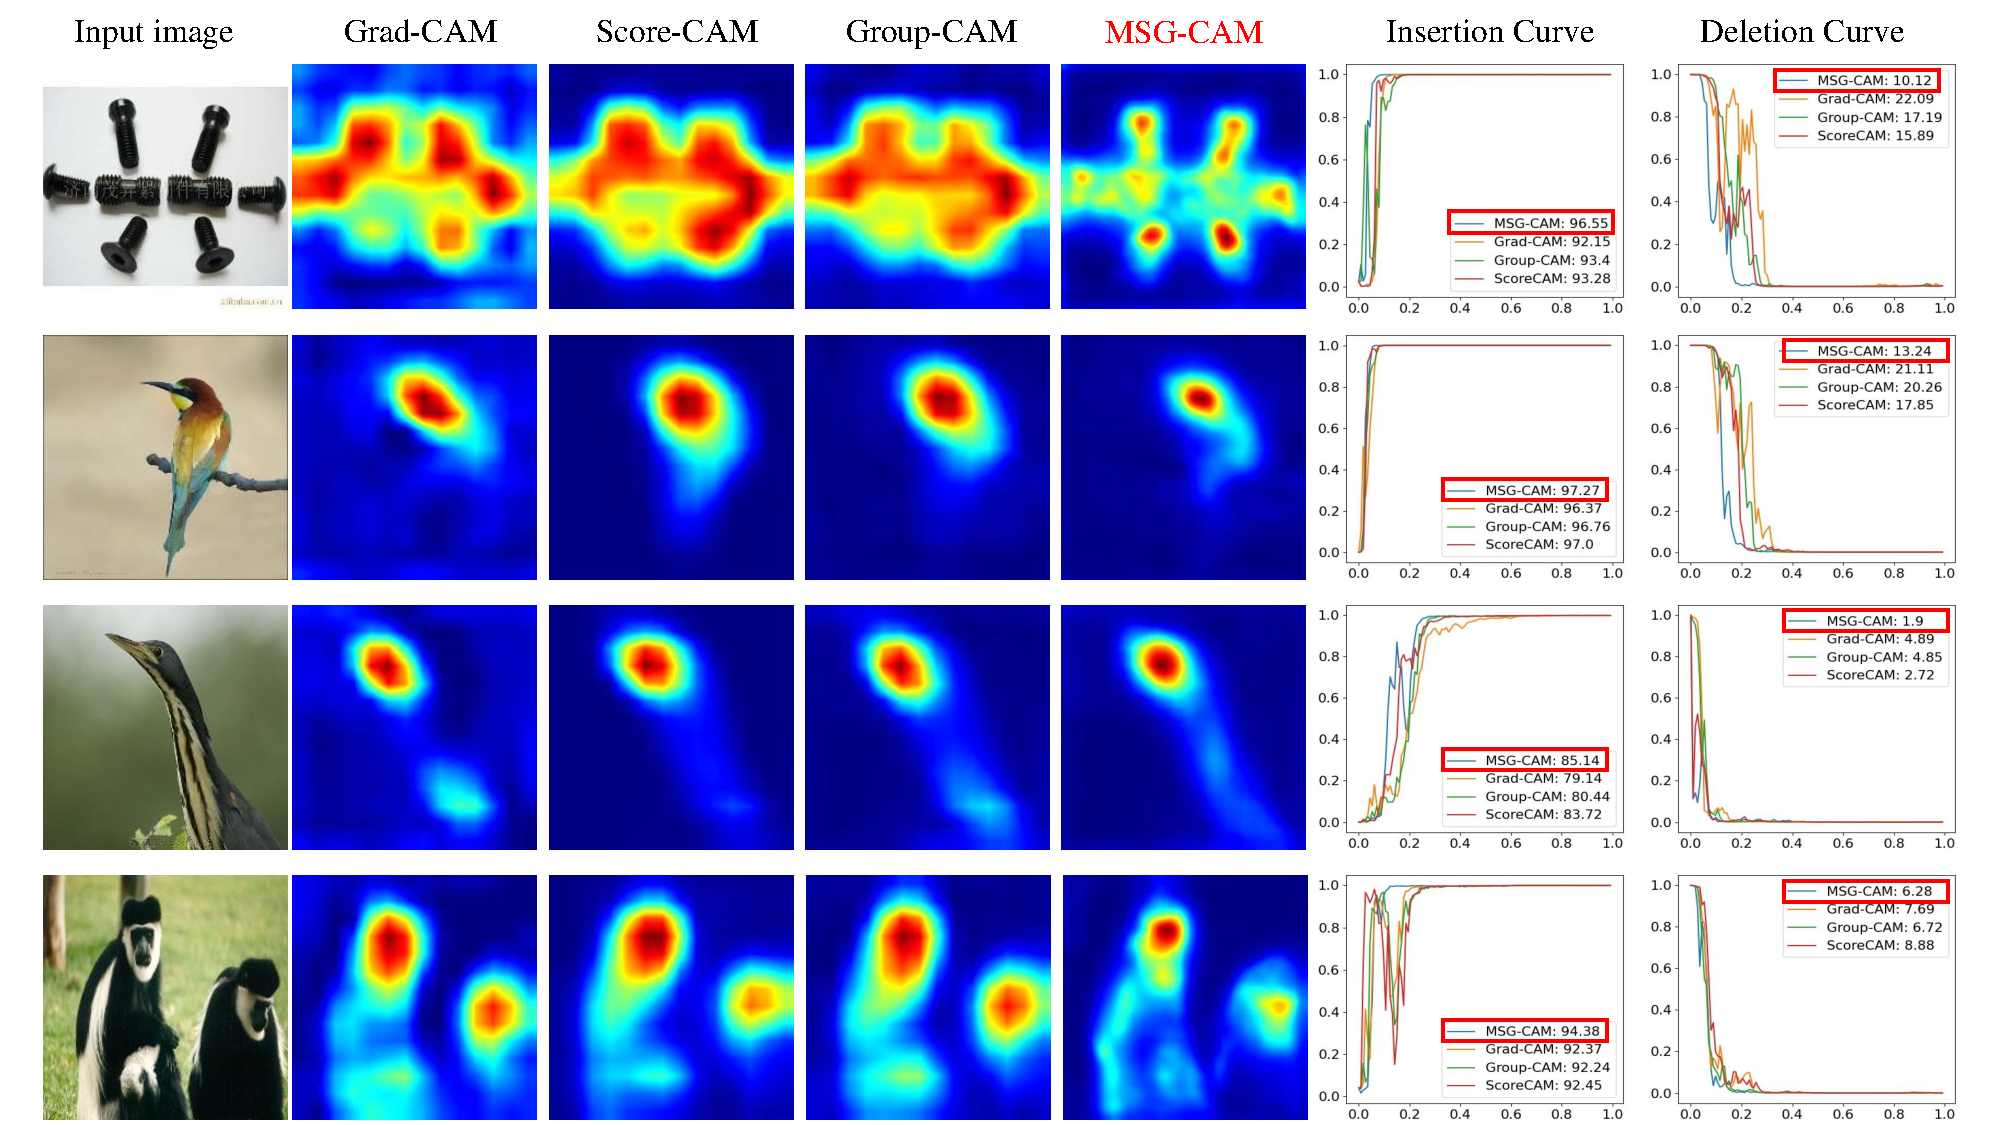
\includegraphics[width=15cm]{fig/ch3/IDCurve.pdf}
	\bicaption[\xiaosi 单张图片在不同方法下的插入删除实验曲线对比]{\wuhao 不同方法下的插入删除实验曲线对比图}{\wuhao Comparison of experimental curves of insertion and deletion under different methods}
%	\bicaption[\xiaosi MSG-CAM算法流程示意图]{\wuhao MSG-CAM算法流程示意图}{\wuhao Pipeline of MSG-CAM}
	\label{fig:IDCurve}
\end{figure}


\begin{table}
	\renewcommand{\arraystretch}{1.5}
	\centering
	\bicaption[\xiaosi 电流类型对效率的影响]{\wuhao 电流类型对效率的影响}{\wuhao Current type impact on efficiency}
	\wuhao
	\label{point}
	\resizebox{\linewidth}{!}{
		\begin{tabular}{llllllll} 
			\toprule
			AUC       & GradCAM & GradCAM++ & XGradCAM & ScoreCAM       & GroupCAM & CAMERAS       & MSGCAM          \\ 
			\toprule
			Insertion & 53.19   & 51.57     & 52.57    & \textbf{55.10} & 54.61    & 44.10         & 54.52           \\
			Deletion  & 11.52   & 12.16     & 11.53    & 11.43          & 11.21    & \textbf{8.01} & 9.78            \\
			Over-all  & 41.67   & 39.41     & 41.04    & 43.67          & 43.40    & 36.09         & \textbf{44.74}  \\
			\bottomrule
		\end{tabular}
	}
\end{table}

\begin{table}
	\renewcommand{\arraystretch}{1.5}
	\centering
	\bicaption[\xiaosi 电流类型对效率的影响]{\wuhao 电流类型对效率的影响}{\wuhao Current type impact on efficiency}
	\wuhao
	\begin{tabular}{ccccccc} %需要10列
		\toprule[1.5pt] %添加表格头部粗线
		\multicolumn{2}{c}{\multirow{2}{*}{Method}}& \multicolumn{2}{c}{PASCAL VOC test}&&\multicolumn{2}{c}{COCO 2014 validation}\\
		\multicolumn{2}{c}{}&&Mean Accuracy($\%$)&&Mean Accuracy($\%$)&\\  %有n个&,就表示该行有n+1列
		\toprule[1.5pt] %绘制一条水平横线
		\multicolumn{2}{c}{Grad-CAM}&   &83.04&    &55.50&    \\   % 占两列,列名为A;后面陆续跟着数字
		\multicolumn{2}{c}{Grad-CAM++}&   &83.21&    &52.91&   \\
		\multicolumn{2}{c}{XGrad-CAM}&   &86.70&    &55.93&   \\
		\multicolumn{2}{c}{Score-CAM}&   &73.92&   &51.20&   \\
		\multicolumn{2}{c}{Group-CAM}&   &82.41&  &54.14&   \\
		\multicolumn{2}{c}{CAMERAS}&   &87.16&    &55.40&   \\
		\multicolumn{2}{c}{\pmb{MSG-CAM}}&   &\pmb{87.24}&   &\pmb{56.62}&   \\
		\bottomrule[1.5pt] %添加表格底部粗线
	\end{tabular}
	\label{point}
\end{table}

\begin{figure*}[htbp]
	\centering
	\bicaption[\xiaosi ]{\wuhao 不同方法下的插入删除实验曲线对比图}{\wuhao Comparison of experimental curves of insertion and deletion under different methods}
	\subfigure[Insertion score divides into segments]{
		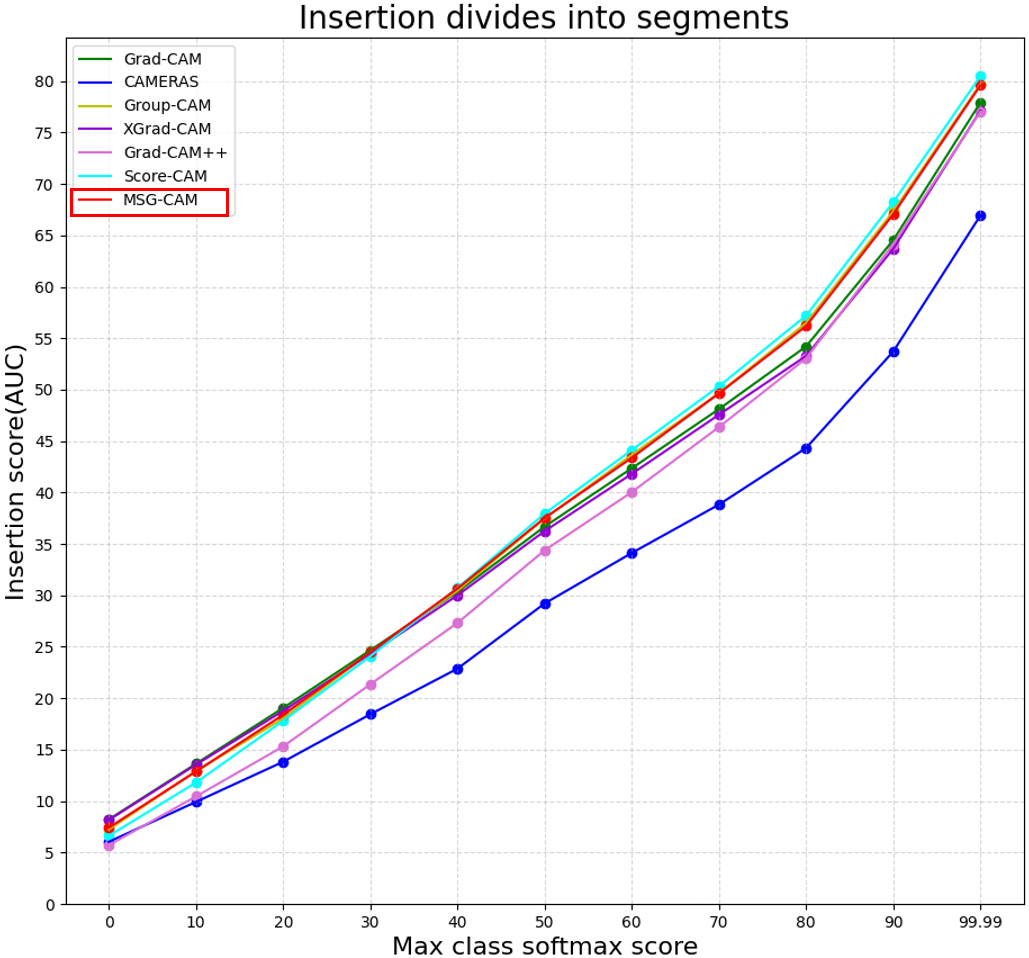
\includegraphics[width=6cm]{fig/ch3/insertion.png}
	}
	\subfigure[deletion score divides into segments]{
		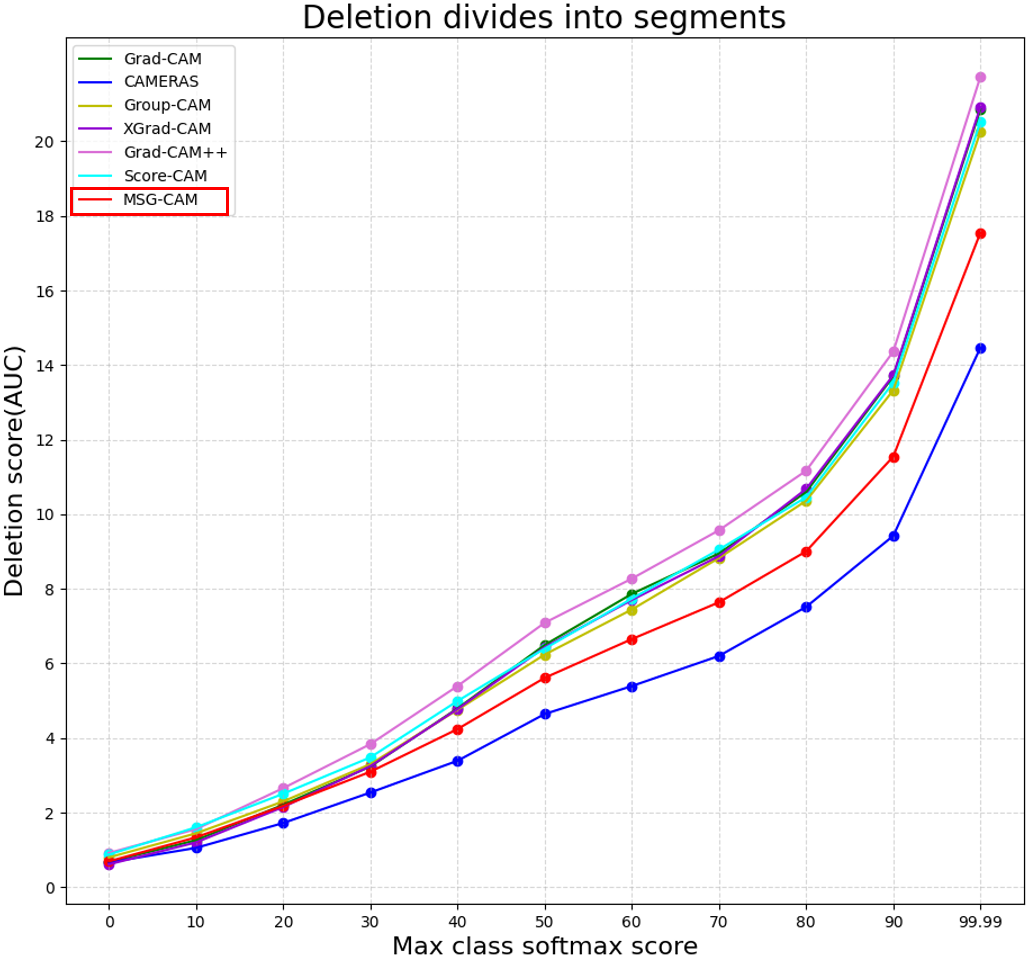
\includegraphics[width=6cm]{fig/ch3/deletion.png}
	}
	\subfigure[over-all score divides into segments]{
		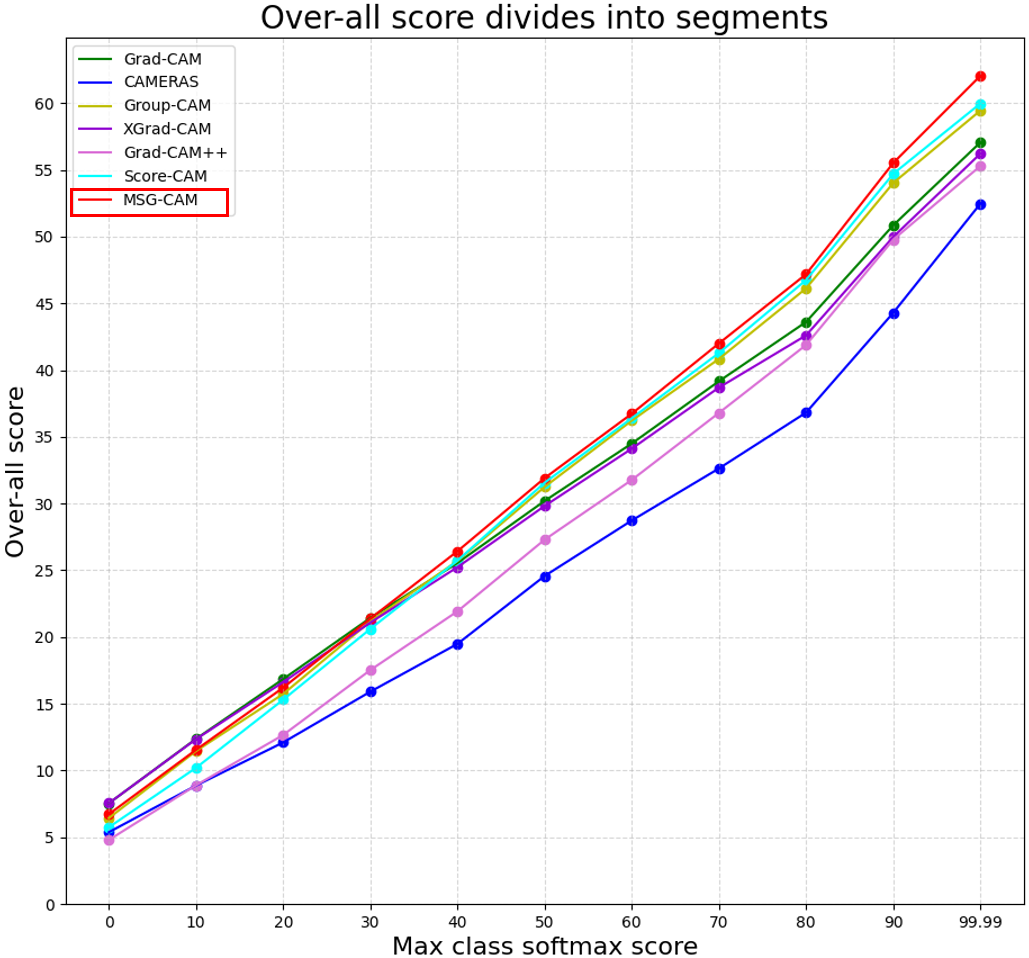
\includegraphics[width=6cm]{fig/ch3/overall.png}
	}
	% \quad
	\label{IDO}
\end{figure*}



\subsection{定点游戏实验}
定点游戏(pointing game)\textsuperscript{\cite{zhang2018top}}实验对于给定显著图解释方法的空间选择性能够给出比较客观的评估结果。所谓空间选择性就是定点游戏要求图像分类神经网络对给定类别在输入图片中指出其所在位置,这对显著图解释方法提出了挑战,方法生成的显著图必须要准确反映给定类别在输入图片的具体位置。定点游戏的具体操作是从针对一个指定类别生成的显著图中找到值最大的那个点并记录它的坐标,如果该坐标位于该类别对象的预先人工标注的边界框内部,则记录一次击中(hit),否则就是没有击中(miss)。定点游戏的量化评价指标即是显著图解释方法在给定数据集上对输入图片中所有类别的击中准确率,具体计算公式如下:
\begin{equation}
	Acc=\frac{\#hits}{\#hits+\#misses}
\label{eq:point}
\end{equation}
在式\ref{eq:point}中,$\#hits$表示数据集中所有显著图的最大值点落在标注框中的个数,$\#misses$则表示数据集中所有显著图的最大值点落在标注框外的个数。在只计算最大值空间选择性的定点游戏当中,$\#hits+\#misses$就等于数据集中所有图片标注框的个数。

为了更加精确的反映显著图的空间选择性,本节实验当中摈弃了只计算最大值点所在坐标的做法,转而计算显著图中里面从大到小的前100个点的坐标,这可以排除偶发性的噪声影响。最终的性能指标是对一个数据集中每个类别的$Acc$取平均。在本次实验中,我们使用的是VGG19模型,且分别在PASCAL VOC测试集和COCO 2014验证集上进行了微调训练。如表\ref{point}所示,我们的方法在两个数据集上都处于领先地位,这表明我们的方法比其他基于类激活映射图的方法更能反映图像分类神经网络的空间选择性。

\subsection{合理性检验}
部分基于反向传播的显著图方法对模型参数并不敏感,这意味不管图像分类模型有没有经过训练,它们都能够给出相似的结果,这显然是违背显著图解释的初衷。所以,能否通过合理性检验是衡量显著图解释方法是否具备可解释性的标准。具体而言,本节~\cite{zhang2018top}根据中的实验方法对经过预训练的VGG19采用级联随机化(cascade randomization)和独立随机化(independent randomization)。级联随机化是从靠近模型的输出端开始,逐渐将卷积层的参数随机化,直至将所有卷积层的参数随机化。 独立随机化也是从靠近模型的输出端开始,每次仅将单独的一层卷积层参数随机化,其他卷积层不变。

图\ref{fig:sanitycheck}中展示了MSG-CAM在单一图片下分别进行级联随机化和独立随机化的结果示意图,图中Conv34表示的是将VGG19的第34层卷积层经过独立随机化和级联随机化后的显著图生成结果,其他的Conv32等以此类推。可以看出无论是级联随机化还是独立随机化,本章提出的MSG-CAM生成的显著图均受到了明显影响,表面MSG-CAM是受到图像分类神经网络训练参数影响的,能够通过合理性检验。

\begin{figure}[h]
	\centering 
	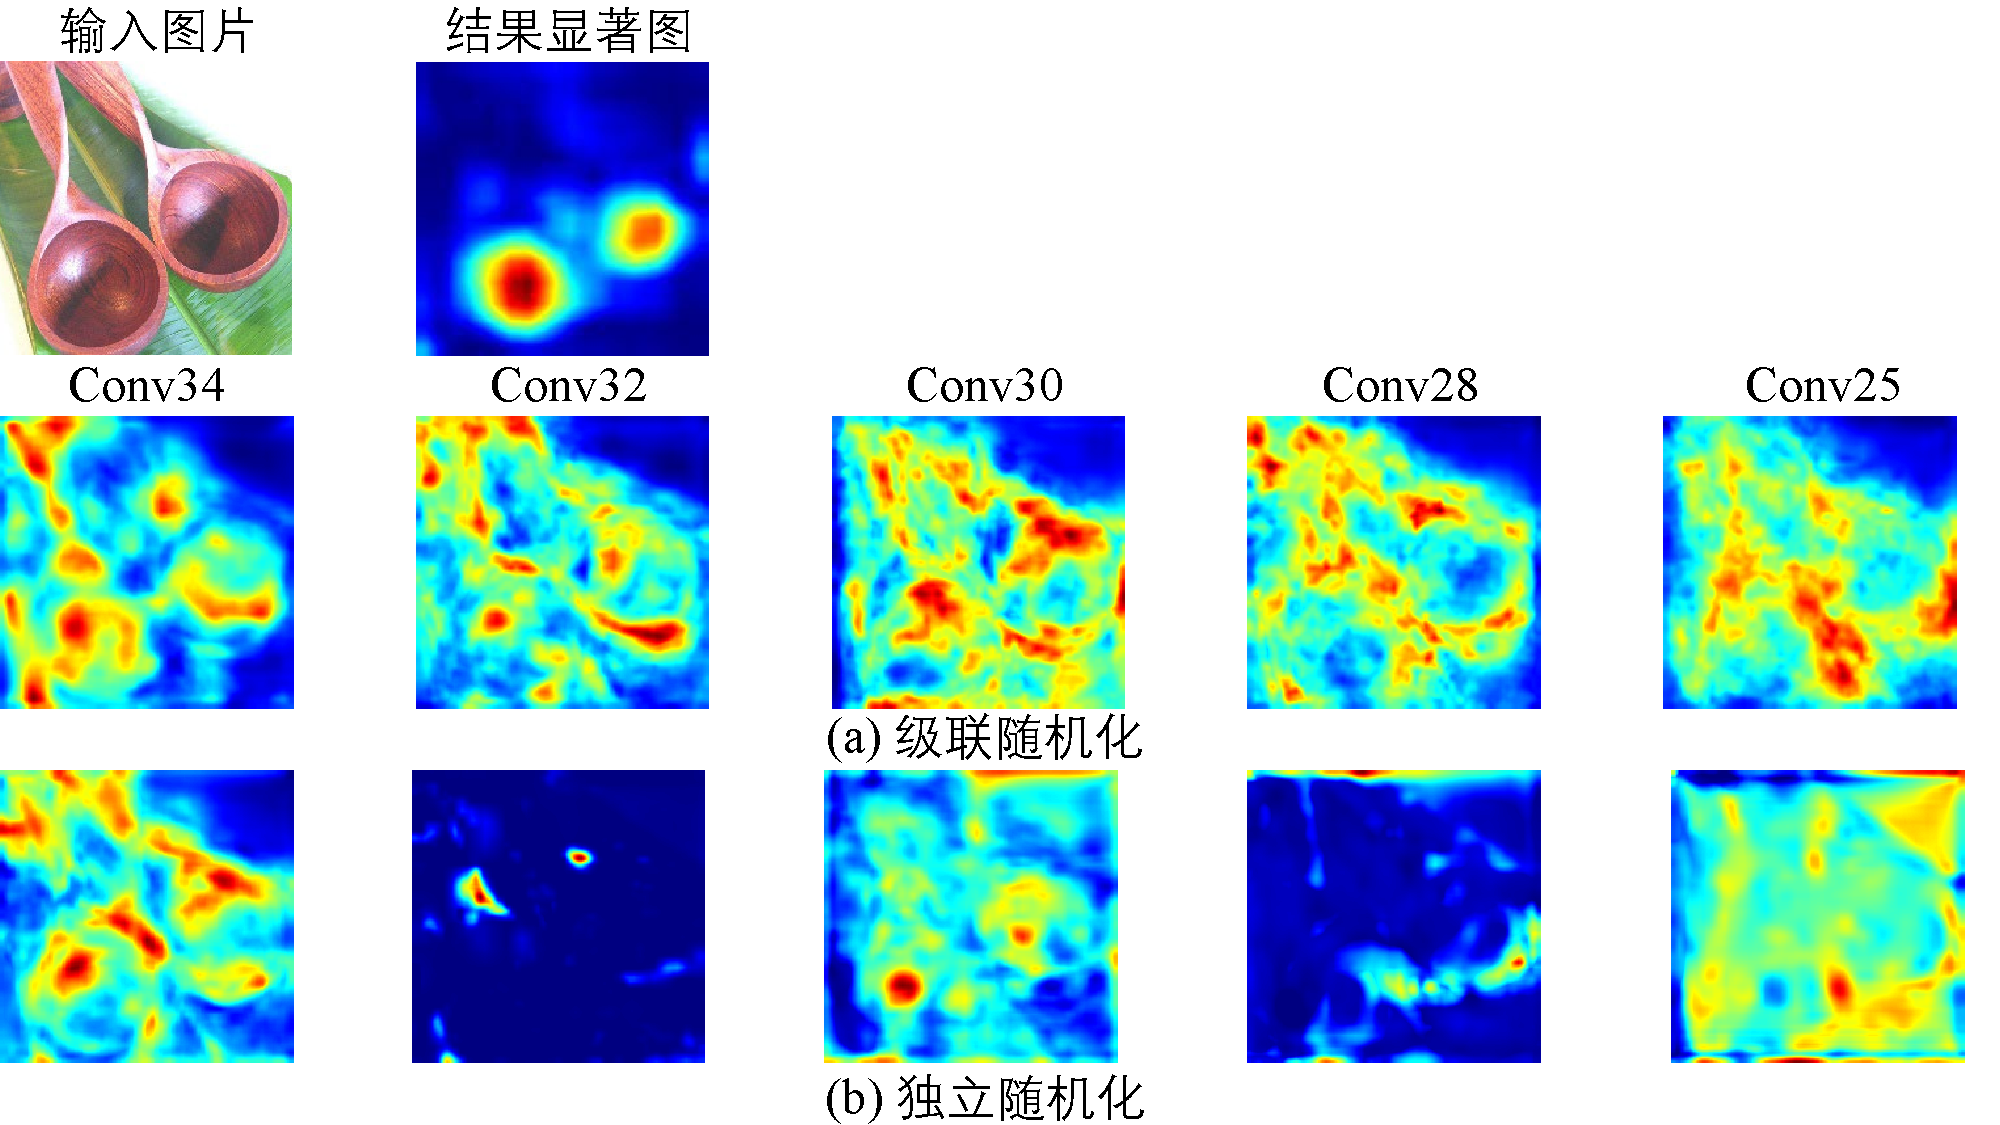
\includegraphics[width=15cm]{fig/ch3/sanityCheck.pdf}
	\bicaption[\xiaosi MSG-CAM合理性检验]{\wuhao MSG-CAM合理性检验示意图}{\wuhao Sanity check of MSG-CAM}
	\label{fig:sanitycheck}
\end{figure}


\section{本章小结}
部分基于反向传播的显著图方法对模型参数并不敏感,这意味不管图像分类模型有没有经过训练,它们都能够给出相似的结果,这显然是违背显著图解释的初衷。所以,能否通过合理性检验是衡量显著图解释方法是否具备可解释性的标准。具体而言,本节~\cite{zhang2018top}根据中的实验方法对经过预训练的VGG19采用级联随机化(cascade randomization)和独立随机化(independent randomization)。级联随机化是从靠近模型的输出端开始,逐渐将卷积层的参数随机化,直至将所有卷积层的参数随机化。 独立随机化也是从靠近模型的输出端开始,每次仅将单独的一层卷积层参数随机化,其他卷积层不变。

图\ref{fig:sanitycheck}中展示了MSG-CAM在单一图片下分别进行级联随机化和独立随机化的结果示意图,图中Conv34表示的是将VGG19的第34层卷积层经过独立随机化和级联随机化后的显著图生成结果,其他的Conv32等以此类推。可以看出无论是级联随机化还是独立随机化,本章提出的MSG-CAM生成的显著图均受到了明显影响,表面MSG-CAM是受到图像分类神经网络训练参数影响的,能够通过合理性检验。

% 第4章




\chapter{基于二维滑动窗口的图像分类神经网络显著图增强方法}
\thispagestyle{others}
\pagestyle{others}
\xiaosi




\section{问题描述和研究思路}

显著图分辨率低,包含特征细节信息少仍然是当前绝大多数显著图解释方法的一个弊病。从基于卷积神经网络的图像分类神经网络来看,针对这一网络的显著图解释方法通常是从卷积神经网络的最后一层卷积层提取特征图。这一层包含了丰富的类别特征信息,然后通过加权组合这些特征图来生成最终的显著图。然而,由于卷积神经网络的结构特性,最后一层卷积层会输出多个通道的低分辨率特征图。因此,无论怎样组合这些特征图,最终得到的显著图分辨率仅与最后一层卷积层的单一通道特征图相当。当然,为了建立显著图与原始输入图片的特征对应关系,通常会对原始输入图片进行分辨率放大。这一过程通常采用双线性插值算法,但这并不意味着显著图中有效信息的增加。另外,当前的一些研究者也在积极探索对基于Tansformer架构的图像分类模型进行显著图解释,H. Chefer等人\textsuperscript{\cite{chefer2021transformer}}在近年发布了针对这一方面的研究,他们针对Transformer的结构的制定了新的层间相关性反向传播规则,解决了传播过程中遇到的注意层和跳跃连接时的挑战。他们将每一个Transformer块的梯度和其对应的相关性分数结合解决了Transformer在图像分类领域的显著图可视化问题。但是即便如此他们针对Transformer提出的方法仍然会面临低分辨率的困扰,究其原因是Transformer结构的图像分类神经网络反向传播过程中计算并生成显著图时也只能受限于token的尺寸,无法生成包含信息量更多的显著图。图\ref{fig:motivation}描述了这一问题,无论针对卷积神经网络的基于类激活映射图的方法还是针对Transformer架构提出的Transformer attribution方法(即Chefer等人提出的方法)都只能生成分辨率较低的原始显著图,之后通过上采样获得最终的显著图。

\begin{figure}[h]
	\centering 
	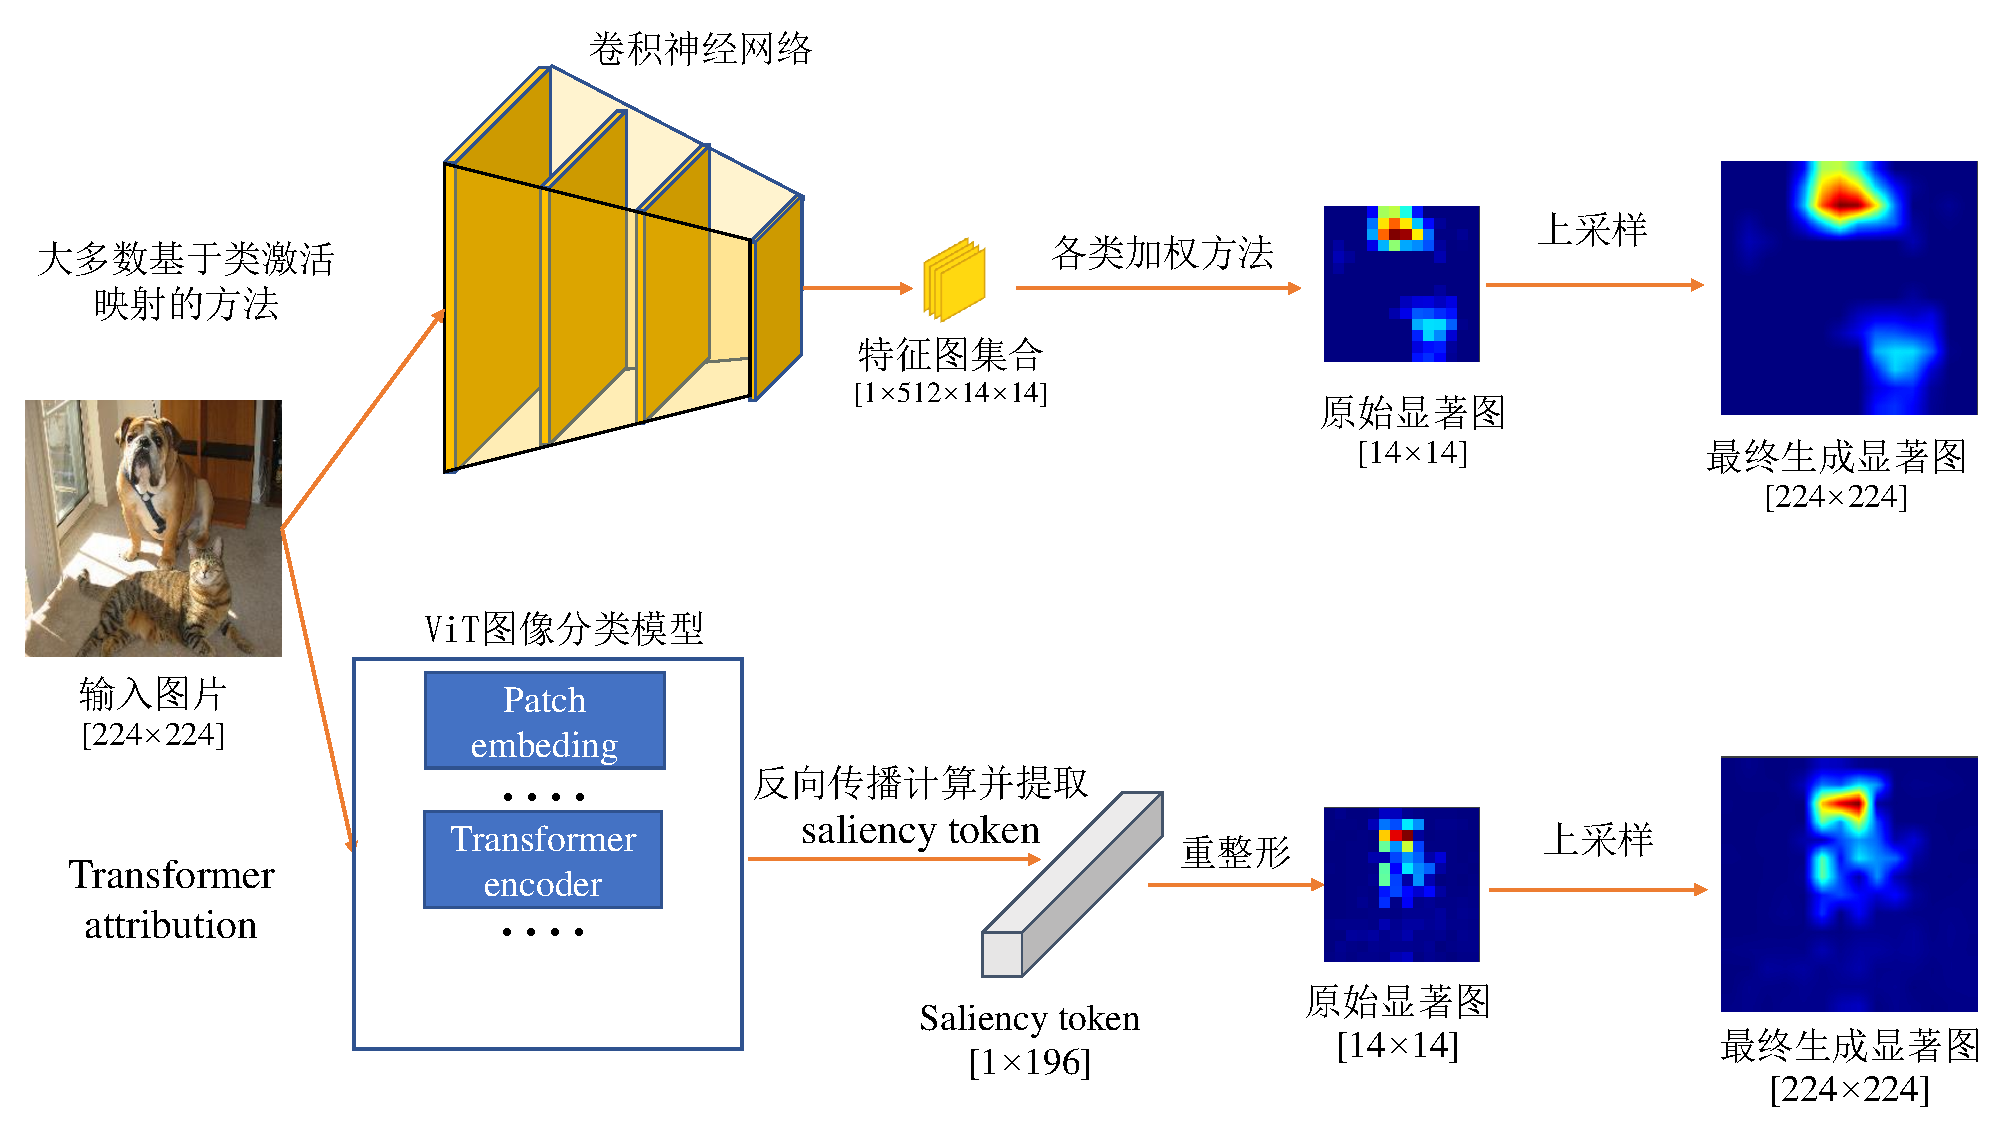
\includegraphics[width=15cm]{fig/ch4/motivation.pdf}
	\bicaption[\xiaosi 当前显著图解释方法分辨低的原因]{\wuhao 当前显著图解释方法分辨低的原因}{\wuhao Reasons for the low resolution of current saliency map interpretation methods}
	\label{fig:motivation}
\end{figure}


因此为了解决上述的问题,本章提出了一种通用的显著图增强方法,可以直接应用在多数可视化算法上。该方法使用固定尺寸的滑动窗口对输入图片中的所有局部区域上采样到输入图片尺寸,然后将结果输入到选定的可视化算法中得到所有图片的针对特定类别的显著图和概率分数,最后将显著图下采样到输入图片对应位置上的窗口中,并乘以概率分数,即可得到具备更多细节的显著图。将该方法应用在不同的可视化算法上,这些算法基于不同架构的网络,无论是量化指标还是直观评测都显示出我们的方法使这些可视化算法得到了明显提升,从而证明本章提出的方法的有效性和可靠性。


\section{基于二维滑动窗口的图像分类神经网络显著图增强方法}
为了解决当前可视化算法存在的分辨率低,特征模糊,噪声多的问题,我们的方法在输入图片上应用了滑动窗口,通过采集并融合不同窗口图片的可视化信息,让可视化算法加强对输入图片中的局部信息的感知。具体的算法流程图展示在图\ref{fig:pipeline}中。

\begin{figure}[h]
	\centering 
	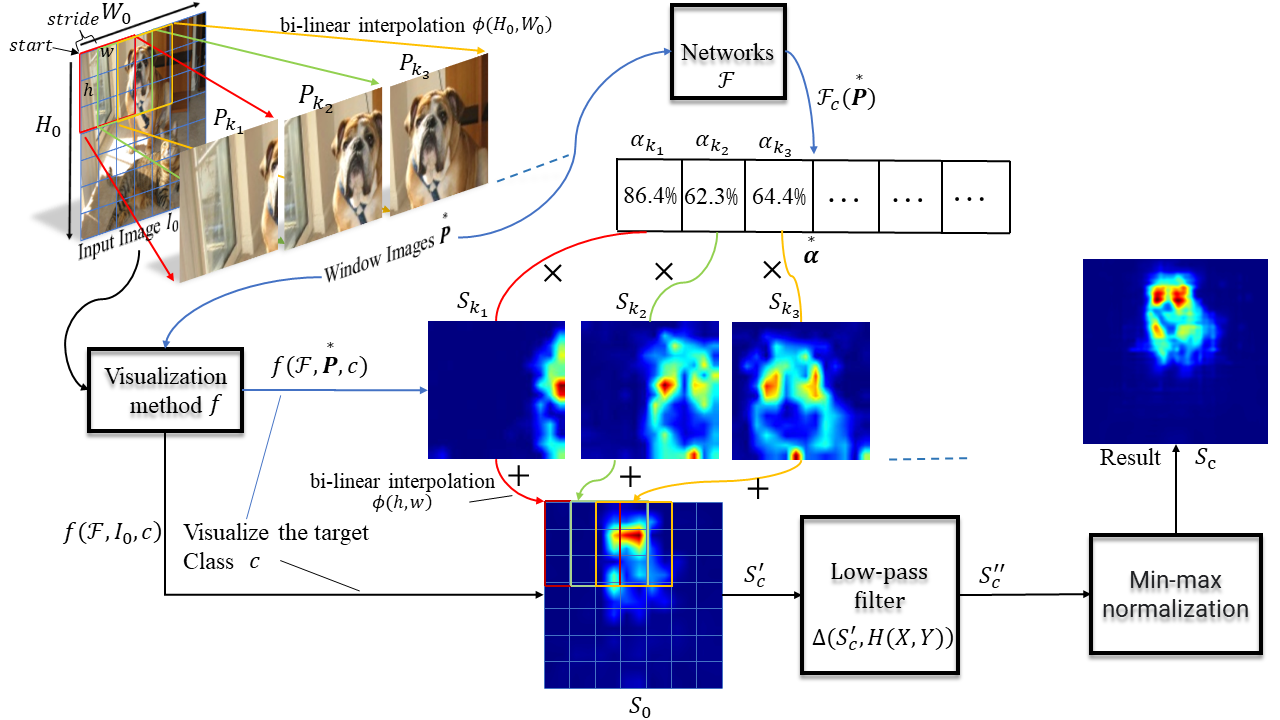
\includegraphics[width=15cm]{fig/ch4/pipeline.png}
	\bicaption[\xiaosi 显著图增强方法的流程图]{\wuhao 显著图增强方法的流程图}{\wuhao Pipeline of the saliency map enhancement approach}
	%	\bicaption[\xiaosi MSG-CAM算法流程示意图]{\wuhao MSG-CAM算法流程示意图}{\wuhao Pipeline of MSG-CAM}
	\label{fig:pipeline}
\end{figure}

\subsection{获取窗口图片集合}
设定原始输入图片$I_0 \in \mathbb{R}^{3\times H_0 \times W_0}$,使用一个二维滑动窗口函数$\psi$来从输入图片$I_0$中提取窗口图片,函数$\psi(I, start, h, w, stride)$中$I$就是函数所应用的输入图片,$start$表示滑动窗口在二维坐标系统的起点,一般设定在输入图片的左上角位置,$h$和$w$表示窗口像素尺寸且窗口尺寸应该小于输入图片尺寸,$stride$表示每次滑动窗口移动的像素个数,窗口从左上角起点开始移动,只能在图片区域内移动,即滑动窗口应该向右或者向左移动。每次移动则将窗口内的图片区域进行复制并保存,移动完毕后即可得到关于窗口图片的集合,单张窗口图片的获取的公式如下:
\begin{equation}
	p_{k_n}=\psi(I_0,start,h,w,stride)
	\label{pkn}
\end{equation}
式\ref{pkn}中$p_{k_n}$表示一张窗口图片,$k_n$表示这张图片在输入图片$I_0$中的二维坐标标记。所有窗口图片的集合可以如下表示:
\begin{equation}
	\overset{*}{\bm{p}}=\{p_{k_1},p_{k_2},\cdots,p_{k_n}\}
\label{ps}
\end{equation}
式\ref{ps}中,$\overset{*}{\bm{p}}$即表示滑动窗口所有窗口图片集合。获取的窗口图片尺寸是和窗口一致的,因此是无法直接输入图像分类模型的,所以需要将其上采样到原始输入图片$I_0$的尺寸,本方法上采样所用的函数是双线性插值函数$\phi$,具体上采样过程描述见如下公式:
\begin{equation}
	\overset{*}{\bm{P}}=\phi(\overset{*}{\bm{p}},H_0,W_0) 
\label{Ps}
\end{equation}
式\ref{Ps}中,$H_0$和$W_0$是原始输入图片$I_0$的长和宽的像素个数,$\overset{*}{\bm{P}}$表示窗口图片上采样后的图片集合,因此 $\overset{*}{\bm{P}}=\{P_{k_1},P_{k_2},\cdots,P_{k_n}\}$,$P_{k_n}$即表示窗口图片$p_{k_n}$上采样到原始输入图片尺寸后的图片。

\subsection{获取窗口图片的显著图和权重}
设定$\mathcal{F}$是经过预训练的图像分类神经网络,$\mathcal{F}_c(I)$表示当输入图片是$I$的情况下,图像分类神经网络$\mathcal{F}$关于类别$c$的输出概率分数。对于当前主流的显著图解释算法来说,将某一显著图解释算法考虑为一个函数$f$,该函数的输入参数是图像分类神经网络$\mathcal{F}$,输入图片$I$和指定类别$c$。当输入图片是$I_0$,可以获得图像分类神经网络$\mathcal{F}$在采用显著图解释算法$f$时生成的关于类别$c$的显著图:
\begin{equation}
	S_0=f(\mathcal{F},I_0,c)
	\label{S0}
\end{equation}
式\ref{S0}是生成的显著图,且$S_0 \in \mathbb{R}^{1\times H_0 \times W_0}$。显著图$S_0$的分辨率和原始输入图片是一致的,因其已经经过上采样处理了。$S_0$中的像素和原始输入图片的像素是一一对应的,且其像素的值表示图像分类神经网络对输入图片$I_0$关于类别$c$的判断权值。现在已经获得了原始输入图片$I_0$的显著图,在上一小节当中,获取的窗口图片集合$\overset{*}{\bm{P}}$也需要经过同样的步骤分别获取每张窗口图片关于类别$c$的显著图:
\begin{eqnarray}
	\overset{*}{\bm{S}} &=& f(\mathcal {F}, \overset{*}{\bm{P}},c) \nonumber \\
	~ &=& \{S_{k_1},S_{k_2},\cdots,S_{k_n}\}
	\label{eq:Ss}
\end{eqnarray}
式\ref{eq:Ss}中$\overset{*}{\bm{S}}$表示图像分类神经网络$\mathcal{F}$对窗口图片集合生成的关于类别$c$的显著图集合,$\overset{*}{\bm{S}}$中所有显著图的分辨率都和原始输入图片$I_0$一致。

在所有基于类激活映射的显著图解释算法中,都采用了各种形式的特征图加权,而这一步骤对于衡量每个特征图关于类别$c$的贡献至关重要。为了衡量由不同窗口图片生成的显著图的重要性,可以获得每张窗口图片相对于类别$c$的概率分数。这个概率分数反映了图像分类神经网络关于窗口图片中类别$c$的特征信息的贡献权重。
\begin{eqnarray}
	\overset{*}{\bm{\alpha}} &=& \mathcal{F}_c(\overset{*}{\bm{P}}) \nonumber \\
	~ &=& \{\alpha_{k_1},\alpha_{k_2},\cdots,\alpha_{k_n}\}
\label{eq:alpha}
\end{eqnarray}
式\ref{eq:alpha}中$\overset{*}{\bm{\alpha}}$就是$\overset{*}{\bm{P}}$所有窗口图片的关于类别$c$的概率分数,以此作为$\overset{*}{\bm{S}}$的权重。

\subsection{融合窗口图片集合的显著图}
由于不同窗口图片生成的显著图只包含了原始输入图片部分区域的特征信息,因此需要将所有窗口图片进行拼接融合从而得到包含丰富特征信息的完整显著图,这一将窗口图片显著图拼接融合的操作也变相提高了最终呈现特征图对细节特征的解释能力,能够给出更精确的特征信息。由于式\ref{eq:ss}中窗口图片显著图集合$\overset{*}{\bm{S}}$中的显著图尺寸和原始输入图片$I_0$的分辨率是一致的,因此要将其下采样至窗口图片的尺寸才方便根据其携带的在原始输入图片中的坐标信息进行拼接融合,具体的过程用公式表示如下:
\begin{eqnarray}
	\overset{*}{\bm{s}} &=& \phi(\overset{*}{\bm{S}},h,w) \nonumber \\
	~ &=& \{s_{k_1},s_{k_2},\cdots,s_{k_n}\}
\label{eq:ss}
\end{eqnarray}
式\ref{eq:ss}中,$\overset{*}{\bm{s}}$是窗口图片集合$\overset{*}{\bm{P}}$的显著图集合$\overset{*}{\bm{S}}$下采样至滑动窗口尺寸的显著图集合,$s_{k_n}$中的$k_n$表示该张显著图在原始输入图片中的坐标位置,这个坐标位置是用来方便后续显著图进行拼接融合的。

显著图拼接融合的具体方法是将所有$\overset{*}{\bm{s}}$中窗口尺寸的显著图乘以该显著图在$\overset{*}{\bm{\alpha}}$对应的权重,再根据记录的坐标和原始输入图片的显著图$S_0$中对应位置区域的像素值相加,窗口显著图拼接融合的具体公式如下:
\begin{eqnarray}
	S^{\prime}_c &=& \sum(\overset{*}{\bm{s}}\overset{*}{\bm{\alpha}}+S_0) \nonumber \\
	~ &=& \sum_{k_1}^{k_n}(\alpha_{k_n}s_{k_n}+S_0^{k_n})
	\label{eq:s'}
\end{eqnarray}
在式\ref{eq:s'}中,$S_0^{k_n}$中$k_n$表示原始输入图片的显著图$S_0$中左上角坐标为$k_n$长宽为$h$和$w$的窗口区域。$S^{\prime}_c$表示拼接融合后的显著图。

\subsection{平滑和归一化显著图}
因为滑动窗口是以一定步长在输入图片上截取窗口图片,这会导致窗口图片的显著图的在按照以上方法进行融合的过程中不可避免的会在拼接融合后的显著图上留下网格状的痕迹,使得显著图视觉效果不够平滑。因此为了尽可能降低滑动窗口带来的不利影响,本方法使用了一个理想低通滤波器对其进行优化,将显著图中网格状的痕迹进行减弱或者消除。定义这个理想低通滤波器函数为$\delta$,$S^{\prime}_c$经过其处理的过程由以下式子定义:

\begin{equation}
	S^{\prime\prime}_c= \Delta(S_c^{\prime},H(X,Y))
	\label{eq:s''}
\end{equation}
式\ref{eq:s''}中,$H(X,Y)$为该理想低通滤波器的传递函数,它的具体定义如下:
\begin{equation}
	H(X,Y)=\left\{
	\begin{aligned}
		1 &&& D(X,Y)\leq D_0 \\
		0 &&& D(X,Y) > D_0
	\end{aligned}
	\right.
	\label{eq:hxy}
\end{equation}
在式\ref{eq:hxy}中,$D_0$是截止频率到频率域中心的距离,它决定了低通滤波器的频率响应范围。当$D(X,Y)$小于$D_0$时,$H(X,Y)$接近于1,表示对低频分量的保留;当$D(X,Y)$大于等于$D_0$时,$H(X,Y)$接近于0,表示对高频分量的抑制。因此,$D_0$决定了滤波器的频率截止位置,即在该位置之前的频率成分会被保留,之后的频率成分会被抑制。$D(X,Y)=\sqrt{X^2+Y^2}$是显著图$S^{\prime}_c$的频率域里的点$(X,Y)$到频率域中心的距离,频率域的中心通常指的是频率域图像的中心点,也就是频率为零的点。

最后,经过低通滤波器处理过后的显著图$S^{\prime\prime}_c$再经过最大最小归一化即可得到增强的且拥有更多特征细节的显著图$S_c$:
\begin{equation}
	S_c=\frac{S_c^{\prime\prime}-min(S_c^{\prime\prime})}{max(S_c^{\prime\prime})-min(S_c^{\prime\prime})}
\end{equation}
 

\section{实验与分析}

\subsection{实验硬件配置和软件环境}
下面给出本章实验的硬件配置和实验环境相关信息,具体信息见表\ref{tab:en1}。
\begin{table}[h]
	\renewcommand{\arraystretch}{1.5}
	\centering
	\bicaption[\xiaosi 实验环境和硬件配置]{\wuhao 实验环境和硬件配置}{\wuhao Experimental environment and hardware configuration}
	\begin{tabular}{p{3cm}p{2.25cm}p{2.25cm}p{2.25cm}p{2.25cm}}
		\toprule[1.5pt]
		\makecell[c]{\songti\wuhao CPU}&\makecell[c]{\songti\wuhao GPU}&\makecell[c]{\songti\wuhao 操作系统}&\makecell[c]{\songti\wuhao Python版本}&\makecell[c]{\songti\wuhao PyTorch版本}\\
		\hline
		\makecell[c]{\wuhao Intel$^\circledR$ Xeon$^\circledR$\\ \wuhao W-2255 CPU\\ \wuhao@3.70GHz}&\makecell[c]{\wuhao NVIDIA \\ \wuhao RTX A5000}&\makecell[c]{ \wuhao  Ubuntu20.04}&\makecell[c]{\wuhao Python3.8}&\makecell[c]{\wuhao 1.10.1+cu113}\\
		\bottomrule[1.5pt]
	\end{tabular}
	\label{tab:en1} 	
\end{table}

\subsection{数据集说明和数据集处理}
在本章的实验当中,主要使用了两个数据集,下面是三个数据集的简要介绍:
1. ILSVRC 2012数据集
ILSVRC 2012(ImageNet Large Scale Visual Recognition Challenge 2012)是一个用于视觉对象识别和定位的大规模数据集和竞赛。该数据集包含超过120万张标注图片,涵盖1000个不同类别的物体和场景。ILSVRC 2012竞赛旨在推动计算机视觉领域的发展,参与者需要开发能够识别图像中物体类别的算法,并对物体进行定位。该竞赛对于深度学习和卷积神经网络等技术的发展起到了重要推动作用,成为了评估图像识别算法性能的重要基准。ILSVRC 2012数据集的发布和竞赛对于推动计算机视觉领域的发展产生了深远影响。

2. ImageNet-Segmentation数据集
ImageNet-Segmentation数据集是由论文\textsuperscript{\cite{guillaumin2014imagenet}}发布的,该论文提出了一种自动填充该数据集的方法,通过像素级的对象-背景分割来丰富图像的注释信息。研究者们通过逐步利用已经分割的图像来引导新图像的分割过程,同时结合类别级别的分割,以实现高质量的分割结果。他们还通过实验证明了该方法在iCoseg数据集上取得了最先进的结果,并且成功地将该方法应用于ImageNet数据集,共包含约50万张图像。最终,他们通过人工标注的方式对445个类别的4276张图像进行了分割,并将这些分割结果整理为ImageNet-Segmentation数据集并发布。

在本章扰动实验中使用的是ILSVRC 2012验证集,包含50000张图片,并且将该验证集中的图片尺寸调整为(3$\times$224$\times$224),其中$3$是表示RGB颜色通道数量,像素值进行归一化调整,调整后的像素值范围是[0, 1],最后使用Imagenet数据集的均值[0.229, 0.224, 0.225]和方差[0.485, 0.456, 0.406]对所有图片像素值进行标准化处理。在图像分割实验当中使用了ImageNet-Segmentation数据集,包含4276张图片,总共445个类别。
\subsection{作为对照的显著图方法}
为了验证本章提出的增强算法,一共选用了5种显著图解释方法来作为对照,本章提出的增强算法将应用在这5种显著图解释方法上来验证增强算法的有效性和可靠性。这5种显著图解释方法分别是:Grad-CAM,Grad-CAM++,LRP,Partial LRP和Transformer attribution。


\subsection{增强方法相关参数}
在本章实验当中,如无特别说明,所有输入图片的尺寸都是$3\times224\times224$,滑动窗口相关参数是:$start=(0,0), h=96, w=96, stride=32$,$start$是输入图片的左上角的像素作为起点 ,也是整个二维坐标系统的起点。低通滤波器的参数设置:$D_0=35$。


\subsection{直观评估}
为了直观评估本章的增强算法生成的显著图效果,本节从ILSVRC 2012验证集中随机选取图片进行了生成显著图的实验。如图\ref{fig:contrast1}和图\ref{fig:contrast2}所示,红色方框中的那列显著图是将本章的增强算法应用到同一种显著图生成方法上得到的。由于LRP算法直接在ViT上的应用效果很差,生成的显著图特征不明显,因此在LRP算法那列下叠加了输入图片作为参照。图\ref{fig:contrast1}和图\ref{fig:contrast2}中可以明显看到,在同一种显著图生成方法下,使用增强算法后的显著图相比没有使用增强算法的显著图呈现出对目标特征轮廓更加清晰的定位,无关的显著高亮区域也更少,能够给用户更加清晰的视觉解释。此外在两种不同架构的图像分类模型ViT和VGG19下,本章的增强算法都能够给出明显的视觉提升效果。例如图\ref{fig:contrast1}中第三行图片,该行的输入图片的类别是“蚯蚓”,在ViT模型下对Transformer attribution方法应用增强算法后生成显著图相比没有使用的增强算法的Transformer attribution方法能够更加清晰的描绘蚯蚓的轮廓特征,这种增强效果同样也反映在VGG19模型下的Grad-CAM方法和Grad-CAM++方法上,这两种方法生成显著图原本只能给出VGG19模型对蚯蚓的左上和右下部分比较关注,却无法得出具体的轮廓细节,在应用本章增强算法后的显著图泽给出了左上和右下明显的蚯蚓轮廓细节。

此外,本节还选取了一些特殊的图片,这些图片中包含模型能够识别出的多个类别的物体。利用这些图片分别对不同的物体的生成显著图可以得到显著图解释算法是否有类别区分性。 如图\ref{fig:classSensitive}所示,红色方框中的仍然是应用本章增强算法后的显著图结果,在第一张输入图片中包含“猫”和“打印机”两个类别,分别对其应用显著图生成方法可以得到图像分类模型对两种类别在输入图片中各自关注的区域。可以看出本章的增强算法依然能够对不同类别的显著图进行增强,例如在第一张输入图片下对VGG19应用Grad-CAM方法,在“打印机”这个类别下的显著图仍然对“猫”这个类别的图片区域进行了高亮突出,在应用增强算法后的显著图则只对“打印机”这个类别的图片区域进行了凸显。这表明本章的增强算法可以对同一张图片中的不同类别的显著图进行增强,给出更加符合模型决策视觉解释。

\begin{figure}[h]
	\centering 
	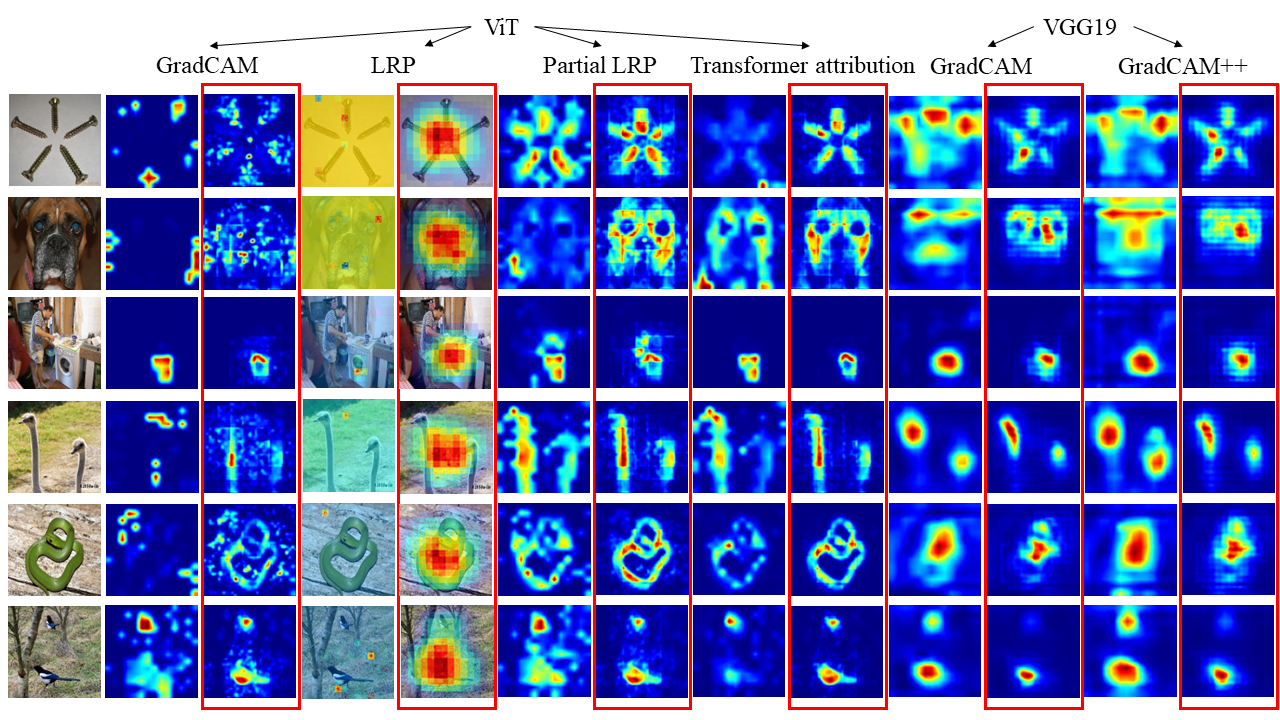
\includegraphics[width=15cm]{fig/ch4/Contrast.png}
	\bicaption[\xiaosi 增强方法应用于多种显著图解释方法上的直观对比结果]{\wuhao 增强方法应用于多种显著图解释方法上的直观对比结果}{\wuhao Intuitive comparison of enhancement methods applied to multiple saliency methods}
	%	\bicaption[\xiaosi MSG-CAM算法流程示意图]{\wuhao MSG-CAM算法流程示意图}{\wuhao Pipeline of MSG-CAM}
	\label{fig:contrast1}
\end{figure}

\begin{figure}[h]
	\centering 
	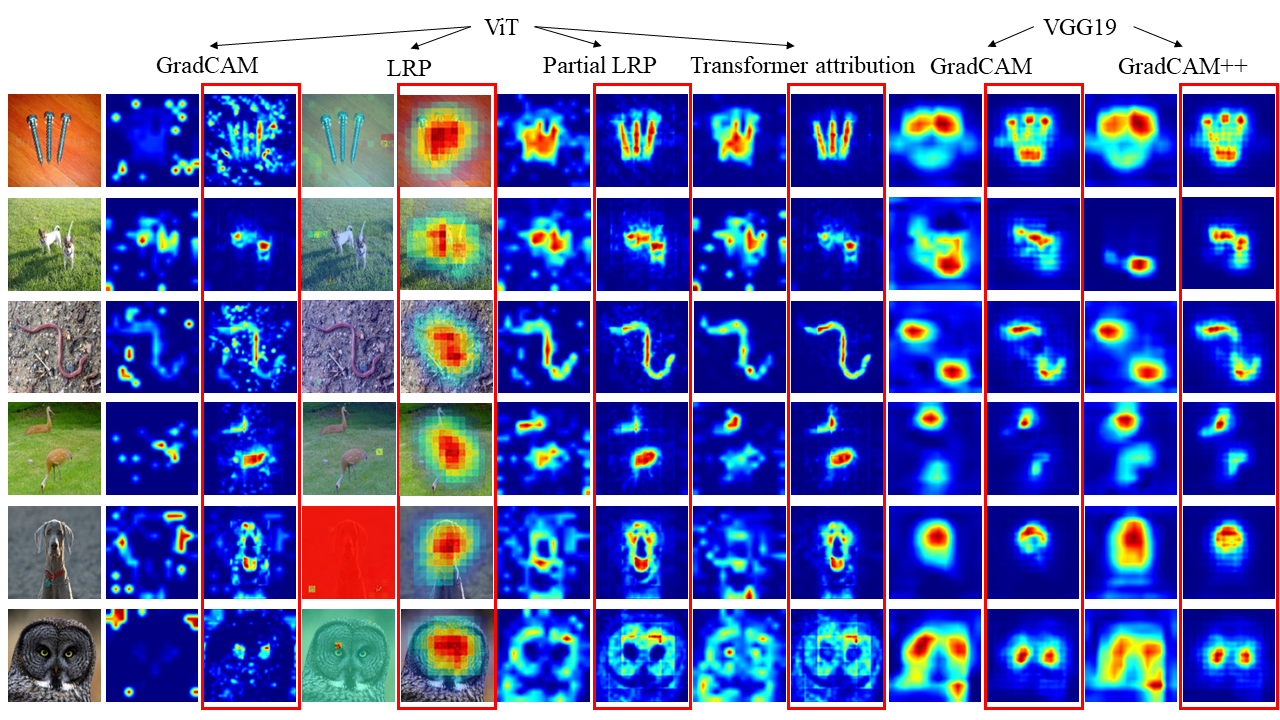
\includegraphics[width=15cm]{fig/ch4/Contrast1.png}
	\bicaption[\xiaosi 增强方法应用于多种显著图解释方法上的直观对比结果]{\wuhao 增强方法应用于多种显著图解释方法上的直观对比结果}{\wuhao Intuitive comparison of enhancement methods applied to multiple saliency methods}
	%	\bicaption[\xiaosi MSG-CAM算法流程示意图]{\wuhao MSG-CAM算法流程示意图}{\wuhao Pipeline of MSG-CAM}
	\label{fig:contrast2}
\end{figure}

\begin{figure}[h]
	\centering 
	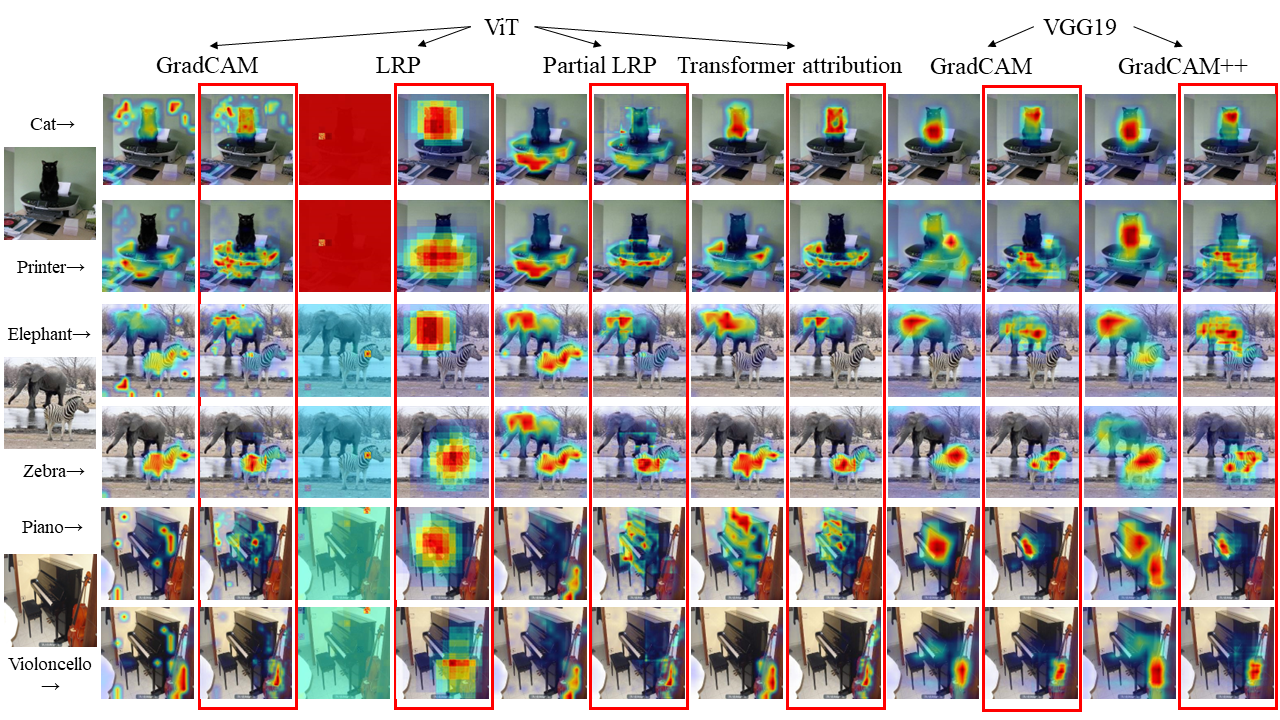
\includegraphics[width=15cm]{fig/ch4/classSensitive.png}
	\bicaption[\xiaosi 增强方法应用于多种显著图解释方法上的类别区分对比]{\wuhao 增强方法应用于多种显著图解释方法上的类别区分对比}{\wuhao Visual comparison of class distinctions of enhancement methods}
	%	\bicaption[\xiaosi MSG-CAM算法流程示意图]{\wuhao MSG-CAM算法流程示意图}{\wuhao Pipeline of MSG-CAM}
	\label{fig:classSensitive}
\end{figure}
\begin{table}
	\centering
	\renewcommand{\arraystretch}{1.5}
	\bicaption[\xiaosi 正负扰动实验数据对比]{\wuhao 正负扰动实验数据对比}{\wuhao Comparison of positive and negative perturbation experimental data}
	\wuhao
	\refstepcounter{table}
	\label{tab:pertubation}
	\resizebox{\linewidth}{!}{
		\begin{tabular}{ccccccccc} 
			\hline
			\multirow{2}{*}{模型}    & \multirow{2}{*}{显著图解释方法}                 & \multirow{2}{*}{增强算法} & \multicolumn{3}{c}{Predicted}                    & \multicolumn{3}{c}{Target}                        \\ 
			\cline{4-9}
			&                                          &                       & 负扰动            & 正扰动            & 总体             & 负扰动            & 正扰动            & 总体              \\ 
			\hline
			\multirow{8}{*}{ViT}   & \multirow{2}{*}{GradCAM}                 &                       & 41.52          & 34.06          & 7.46           & 42.02          & 33.56          & 8.46            \\ 
			\cline{4-9}
			&                                          & \checkmark                     & \textbf{47.54} & \textbf{26.99} & \textbf{20.55} & \textbf{48.46} & \textbf{26.49} & \textbf{21.97}  \\ 
			\cline{2-9}
			& \multirow{2}{*}{LRP}                     &                       & 43.49          & 41.94          & 1.55           & 43.49          & 41.94          & 1.56            \\ 
			\cline{4-9}
			&                                          & \checkmark                     & \textbf{62.69} & \textbf{27.51} & \textbf{35.18} & \textbf{64.76} & \textbf{26.45} & \textbf{38.31}  \\ 
			\cline{2-9}
			& \multirow{2}{*}{partial LRP}             &                       & 50.49          & 19.64          & 30.85          & 50.49          & 19.64          & 30.85           \\ 
			\cline{4-9}
			&                                          & \checkmark                     & \textbf{55.57} & \textbf{18.45} & \textbf{37.12} & \textbf{56.13} & \textbf{18.14} & \textbf{37.99}  \\ 
			\cline{2-9}
			& \multirow{2}{*}{Transformer attribution} &                       & 54.14          & 17.03          & 37.11          & 55.04          & \textbf{16.04} & 39.00           \\ 
			\cline{4-9}
			&                                          & \checkmark                     & \textbf{57.57} & \textbf{16.93} & \textbf{40.64} & \textbf{58.83} & 16.25          & \textbf{42.58}  \\ 
			\hline
			\multirow{4}{*}{VGG19} & \multirow{2}{*}{GradCAM}                 &                       & 38.08          & 12.15          & 25.93          & 39.04          & 11.71          & 27.33           \\ 
			\cline{4-9}
			&                                          & \checkmark                     & \textbf{39.07} & \textbf{10.20} & \textbf{28.87} & \textbf{40.09} & \textbf{9.78}  & \textbf{30.31}  \\ 
			\cline{2-9}
			& \multirow{2}{*}{GradCAM++}               &                       & 40.50          & 11.79          & 28.71          & 40.81          & 11.61          & 29.20           \\ 
			\cline{4-9}
			&                                          & \checkmark                     & \textbf{40.95} & \textbf{10.09} & \textbf{30.86} & \textbf{41.49} & \textbf{9.81}  & \textbf{31.68}  \\
			\hline
		\end{tabular}
	}
\end{table}
\subsection{扰动实验}
优秀的显著图解释算法要能准确找到神经网络做出决策的关键特征,并且在生成的显著图中对每个像素赋予它与其对决策贡献相匹配的数值。扰动实验就是在这一标准上比较不同显著图解释算法的性能。我们分别进行正负扰动实验,正负实验测试采用两阶段设置。首先,使用预先训练好的网络提取 ImageNet验证集的可视化图像。其次,逐渐屏蔽掉输入图像的像素,并测量网络的平均top-1准确率。在正扰动实验中,像素从相关度最高的像素被屏蔽到最低的像素,而在负扰动中,像素从最低的像素被屏蔽到最高的像素。在正向扰动中,我们会看到性能急剧下降,这表明被遮挡的像素对分类得分很重要。在负扰动实验情况下,一个好的解释可以保持模型的准确性,同时去除与类别无关的像素。在这两种情况下,我们都测量了去除10\%-90\%像素时的曲线下面积(AUC)。这两项实验都可应用于图像分类模型预测结果类(Predicted)和真实标注类(Target)。在后一种情况下,特定类别的方法有望获得更好的性能,而与类别无关的方法则会在两种测试中表现出相似的性能。

正负扰动实验和插入删除实验本质是一致的,都是根据显著图给出的像素权值将输入图片中的像素删除来记录得到相关类别索引的概率分数的变化。在正负扰动实验当中,也可以用AUC(总体)来综合评价扰动实验结果,它的计算方式是AUC(总体)=AUC(负扰动)-AUC(正扰动)。从表1中可以看出,我们的增强算法在overall指标上都取得明显提升,其中提升最为显著的是ViT模型的可视化算法GradCAM和LRP,这是因为他们对ViT的可视化能力很差,无法定位关键特征,经过我们的方法增强后,初步具有定位关键特征的能力。这表明我们的方法可以帮助这些可视化算法找到神经网络感兴趣的关键特征,这在不同的模型上都是成立的。

从表\ref{tab:pertubation}中可以看出,我们的增强方法显著提高了所有"总体"得分。应用于ViT的Grad-CAM 算法和LRP算法的改进最为明显,这两种算法以前缺乏准确可视化和定位重要特征的能力。使用增强方法后,这些方法能够识别重要特征。图\ref{fig:contrast1}就是一个例子,它表明无论底层网络结构如何,我们的方法都能帮助显著性方法识别神经网络感兴趣的重要特征。






\begin{table}
	\renewcommand{\arraystretch}{1.5}
	\centering
	\bicaption[\xiaosi 显著图增强算法在图像分割的表现]{\wuhao 不同的显著图解释方法应用增强算法前后图像分割的表现}{\wuhao Performance of saliency map enhancement algorithms for image segmentation}
	\wuhao
	\label{tab:seg}
	\resizebox{\linewidth}{!}{
		\begin{tabular}{cccccc} 
			\hline
			模型                     & 显著图解释方法                                  & 增强算法 & Pixel Acc(\%)      & mAP(\%)             & mIoU(\%)             \\ 
			\hline
			\multirow{8}{*}{ViT}   & \multirow{2}{*}{GradCAM}                 &      & 64.44          & 71.60          & 40.82           \\ 
			\cline{3-6}
			&                                          & \checkmark    & \textbf{70.33} & \textbf{77.02} & \textbf{47.81}  \\ 
			\cline{2-6}
			& \multirow{2}{*}{LRP}                     &      & 51.09          & 55.68          & 32.89           \\ 
			\cline{3-6}
			&                                          & \checkmark    & \textbf{69.34} & \textbf{80.88} & \textbf{50.37}  \\ 
			\cline{2-6}
			& \multirow{2}{*}{partial LRP}             &      & 76.31          & 84.67          & 57.94           \\ 
			\cline{3-6}
			&                                          & \checkmark    & \textbf{80.42} & \textbf{85.83} & \textbf{62.85}  \\ 
			\cline{2-6}
			& \multirow{2}{*}{Transformer attribution} &      & 79.74          & 86.03          & 62.01           \\ 
			\cline{3-6}
			&                                          & \checkmark    & \textbf{81.90} & \textbf{86.56} & \textbf{64.56}  \\ 
			\hline
			\multirow{4}{*}{VGG19} & \multirow{2}{*}{GradCAM}                 &      & 69.03          & 76.76          & 48.99           \\ 
			\cline{3-6}
			&                                          & \checkmark    & \textbf{73.78} & \textbf{79.99} & \textbf{53.82}  \\ 
			\cline{2-6}
			& \multirow{2}{*}{GradCAM++}               &      & 76.77          & \textbf{85.48} & 58.89           \\ 
			\cline{3-6}
			&                                          & \checkmark    & \textbf{78.60} & 85.42          & \textbf{60.58}  \\
			\hline
		\end{tabular}
	}
\end{table}


\subsection{图像分割实验}
图像分割实验将每张显著图视为图像的软分割,并将其与ImageNet-Segmentation数据集的真实标注的分割进行比较。在分割实验中,计算每个突出图中像素的平均值,并将突出图中高于平均值的像素设为 1,其余像素设为 0。本节使用语义分割中常用的三个指标来衡量性能:像素精确度(Pixel Accuracy)、平均交叉重叠率(mIoU)和平均精确度(mAP),其中mIoU即对每张显著图进行平均值阈值化处理后获得的准确度,mAP是使用不含阈值的显著图计算得出的。

分割结果如表\ref{tab:seg}所示。从中可以看出,我们的增强方法在所列的像素精确度(Pixel Accuracy)、平均交叉重叠率(mIoU)和平均精确度(mAP)关键指标,上都有显著的改进,甚至 Transformer attribution\textsuperscript{\cite{chefer2021transformer}} 也能获得不可忽略的改进,这是目前在基于Transformer架构上的图像分类神经网络ViT模型上表现最好的方法。这表明,本章的增强方法可以帮助提高当前显著图解释方法在分割领域的性能。

	
\section{本章小结}
本章首先分析当前显著图生成方法普遍存在的低分辨率问题的原因,然后本章详细介绍了一种通用的基于二维滑动窗口和放大的图像分类神经网络显著图解释增强方法,该方法无须改变当前既有的显著图生成方法的内部计算流程,只需要关注输入的原始图片和输出的概率分数即可完成对当前既有显著图生成方法的增强。增强后的显著图具有更高的分辨率和更精准的特征定位。为了使得因滑动窗口导致的显著图不够平滑的问题,本章的方法还使用了低通滤波器对其平滑。最后本章设计了扰动实验,选取了多个显著图生成方法和两个不同架构的图像分类网络来验证本章增强方法的有效性,经过直观对比和数据对比,本章的显著图增强方法都取得了明显效果。 



\chapter{显著图解释方法对比评测系统}
\thispagestyle{others}
\pagestyle{others}
\xiaosi




当前存在众多的显著图解释方法,但是许多方法由于代码编写复杂,或者方法的作者提供的接口不统一,难以直观的对比不同的显著图解释方法在相同条件下的性能。因此本章将许多已有的显著图解释方法统一程序接口,并结合软件可视化开发技术开发了一套显著图解释方法对比评测系统,该系统可以方便研究人员对当前显著图解释方法进行对比评测,直观展现不同显著图解释方法在相同条件下的视觉差别和评测指标差异。

\section{系统需求分析}

本系统的功能目标主要是方便对比不同的显著图解释方法。通过导入模型设置显著图解释方法的参数可以针对性地适应不同显著图解释方法在不同模型下的表现要求;通过选择特定的图片生成显著图可以直观对比不同显著图解释方法的显著图;通过利用生成的显著图可以对原始输入图片进行图像分割直观对比不同显著图解释方法对目标物体的特征捕获能力;通过选定实验类型和数据集可以比较不同显著图解释方法在相同评价指标的性能表现;可以分别导出备份显著图解释方法的的性能评测指标相关数据。

本系统主要包含以下几个功能模块,每个功能模块的需求信息如下: 

 1.用户登录注册模块:用户可以注册账号,之后可以利用账号密码登录系统。
 
 2.信息设置模块:在模型设置当中用户可以将本地的模型文件上传导入到系统当中,并可以修改模型名称;在显著图解释方法设置当中用户可以根据不同的模型对应的显著图解释方法设置相关必须参数,例如选择卷积层等;在账号设置当中用户可以查看密码更改密码。

 3.显著图生成模块:在该模块中,用户可以从下拉框中选定要使用的图像分类模型,之后可以从本地选择要生成显著图的输入图片,点击生成预测类别的按钮即可得到当前模型对该图片的前几名类别和对应的概率,用户可以从下拉框中选择要生成显著图的类别,之后从下拉框中选择要使用的显著图解释方法,此处选择的显著图解释方法会自动应用显著图解释方法设置中的对应的参数,最后点击生成显著图即可在页面中生成当前显著图解释方法在选定类别索引下的显著图。
 
 4. 显著图切割模块:在这个模块中,用户可以选择图像分类模型,并从本地选择输入图片,然后点击生成预测类别的按钮,得到当前模型对该图片的前几个类别和对应的概率。用户可以选择类别并生成对应的显著图,然后选择要使用的显著图解释方法。所选的显著图解释方法将自动应用设置中的相应参数。页面会展示已经生成的显著图,此时用户可以选择将显著图中对应原始输入图片的重要区域单独分割出来,分割的比例可以从下拉框中选择。用户还可以选择不同的显著图解释方法直观对比不同显著图解释方法的分割效果。
 
 5.实验测试模块:在该模块中用户可以选择数据库中既有的图像分类模型其中也包括用户自行上传的模型,之后选择要进行的实验类型,其中包括几种主流的实验有插入删除实验,分割测试实验等,最后选择显著图解释方法即可进行实验,实验结束后会将实验数据结果显示给用户,并存入用户对应的数据库中。
 
 6.备份保存模块:用户可以把在实验测试模块中的数据进行备份保存,保存方式是纯文本形式,包括实验时间,实验结果,实验相关参数等。

\begin{table}
	\renewcommand{\arraystretch}{1.5}
	\centering
	\bicaption[\xiaosi 软件开发环境和硬件配置]{\wuhao 软件开发环境和硬件配置}{\wuhao Software development environment and hardware configuration}
	\label{tab:sys}
	\begin{tabular}{p{4cm}p{8cm}} 
		\hline
		配置                     & \multicolumn{1}{c}{详情}             \\ 
		\hline
		\multirow{9}{*}{服务端配置} & CPU:10-core Intel$^\circledR$ Xeon$^\circledR$ W-2255 CPU  \\
		& 内存:128GB 64-bit DDR4 3700MHz       \\
		& 显卡:NVIDIA RTX A5000 24GB           \\
		& 操作系统:Ubuntu 20.04 LTS              \\
		& Python版本:Python3.8                 \\
		& 深度学习框架:Pytorch 1.10.1              \\
		& 计算架构:CUDA 11.4                     \\
		& 计算加速库:CUDNN 8.2.0                  \\
		& AI性能:27.8 TFLOPS                   \\ 
		\hline
		\multirow{7}{*}{开发端配置} & CPU:AMD Ryzen 5 4600U              \\
		& 内存:16GB 64-bit LPDDR4 3200MHz      \\
		& 操作系统:Windows11 家庭中文版               \\
		& Python版本:Python3.8                 \\
		& PyQt版本:PyQt5                       \\
		& 数据库:MySQL 5.5                      \\
		& 集成开发环境:PyCharm社区版2021.2.3            \\
		\hline
	\end{tabular}
\end{table}

 
\section{开发环境及相关技术介绍}
本章的系统由于采用客户端/服务器架构,所以软件硬件环境也分为服务端和客户端。在服务端主要是执行计算量较大的关于深度神经网络的计算,客户端主要是负责页面展示和功能选择。本系统的开发端即可看作客户端,开发的客户端即在开发端运行。  具体配置要求如表\ref{tab:sys}所示。



本章的系统使用了PyQt作为前端图形开发框架,在此对其进行简要的介绍。PyQt是一个用于创建图形用户界面(GUI)应用程序的开发框架,它基于Qt库和Python语言。PyQt提供了丰富的工具和组件,使开发者能够快速、灵活地构建跨平台的应用程序。它包括了用于创建窗口、按钮、菜单、对话框等各种GUI元素的类和方法,同时也支持事件处理、信号与槽机制,以及与数据库、网络等其他模块的集成。PyQt还提供了对Qt Designer的支持,可以通过可视化界面设计工具来快速布局和设计界面。由于PyQt基于Qt库,因此能够充分利用Qt的强大功能和跨平台特性,使开发者能够轻松地将应用程序部署到不同的操作系统上。总之,PyQt是一个功能强大、灵活且易于使用的图形开发框架,适用于各种规模和类型的应用程序开发。

\section{系统设计}
\subsection{系统架构设计}
本系统采用经典的C/S架构设计,即客户端/服务器架构。由于显著图解释方法所需的图像分类模型较多较杂,需要依赖的外围软件较多,计算量较大,因此直接在用户的本地客户端运行显著图解释方法实现难度较大。所以该系统架构将主要的逻辑功能实现放在后台服务器端,用户在客户端操作将相关操作指令通过网络上传后台服务器,由服务器处理完成后传输数据给客户端展示。客户端/服务器架构模式有利于后期维护和功能升级。

本系统的整体系统架构可以从下到上可以分为四个层次,分别是:基础平台、软件平台、功能逻辑和前端页面。每个层次包含的模块内容如图\ref{fig:sys}所示:

\begin{figure}[h]
	\centering 
	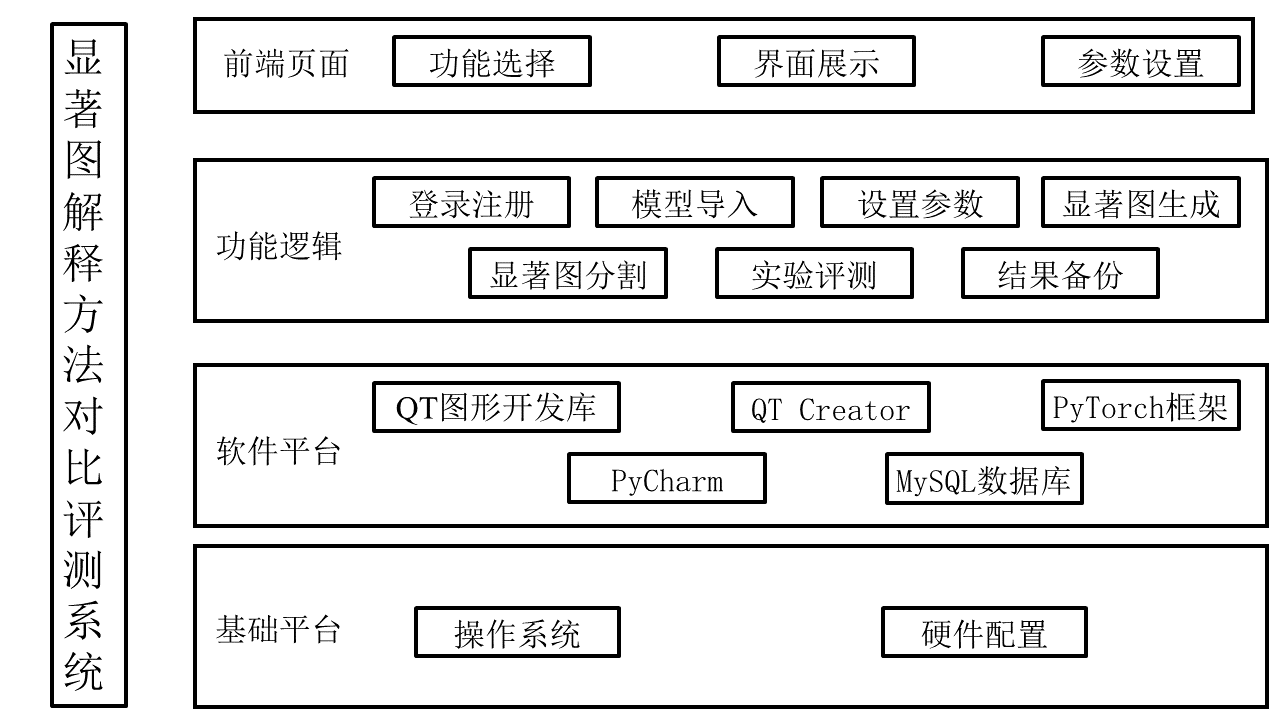
\includegraphics[width=15cm]{fig/ch5/sys.png}
	\bicaption[\xiaosi 系统架构设计图]{\wuhao 系统架构设计图}{\wuhao System Architecture Design Diagram}
	\label{fig:sys}
\end{figure}
\subsection{模块设计}
显著图解释方法对比评测系统的主要功能可以分为用户功能模块和主要系统功能模块。用户功能模块包括用户登录注册、用户修改账号密码、模型查看和导入、显著图解释方法参数设置、用户评测数据备份。主要系统功能模块包括显著图方法生成对比、显著图方法分割对比、显著图方法实验评测。

显著图解释方法对比评测系统的模块设计图如图\ref{fig:function}所示,用户需要注册登录才能使用系统主要功能,用户的相关个人信息保存在服务端的数据库中,服务端和客户端通过http协议进行通信。

\begin{figure}[h]
	\centering 
	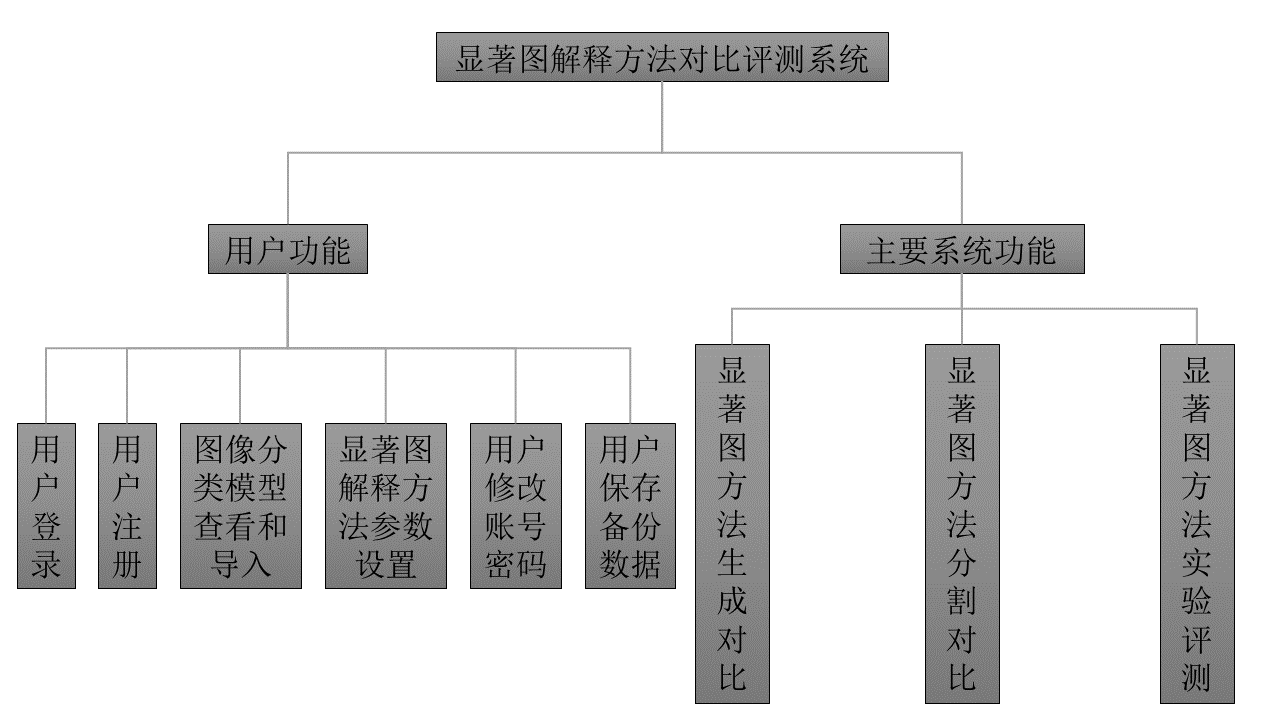
\includegraphics[width=15cm]{fig/ch5/function.png}
	\bicaption[\xiaosi 系统模块设计图]{\wuhao 系统模块设计图}{\wuhao System Module Design Diagram}
	\label{fig:function}
\end{figure}

\subsection{功能设计}

本系统包含众多的分支功能,下面是对每个功能的详细描述:

1.用户注册登录功能

为了记录每个用户的实验数据和显著图解释方法的配置信息,每个用户都需要注册并登录,注册后每个用户有唯一的用户账号用来在服务端数据库中保存相关实验数据。注册用户需要自定义唯一的用户名和设置登录密码,注册成功后系统会生成唯一的数字账号。后续登录功能时用户可以用用户名和数字账号进行登录。

2.图像分类模型的查看和导入

在用户登录后,用户需要在信息设置中查看当前服务端可用的图像分类神经网络模型,用户也可自行上传合适的图像分类神经网络模型到服务端。
目前可用的图像分类模型包括:VGG16、VGG19、ResNet18、ViT。

3.显著图解释方法的参数设置
 
在显著图解释方法的参数设置当中,用户可以看到当前可用的显著图解释方法,对于每一种显著图解释方法,用户可以自行设置参数,可以针对每一种图像分类神经网络的参数设置都会被保存到服务端,后续显著图生成选择显著图解释方法时会自动应用用户的参数设置信息,并且会根据用户选择的图像分类模型进行参数调整。目前可用的显著图解释方法包括:Grad-CAM、Grad-CAM++、Score-CAM、XGrad-CAM、RISE、Transformer Attribution、MSG-CAM。除此之外还包括本文第四章提出的增强方法,该显著图增强方法可以直接应用于上述显著图解释方法。

4. 显著图生成功能

显著图生成功能主要是方便用户在单一图片情况下直接对比不同显著图解释方法的生成效果。用户首先需要选定图像分类模型,再选择输入图片,输入图片可以从用户本地上传,选定输入图片后页面会显示用户的输入图片。然后用户需要点击按钮将该图片输入到选定的图像分类模型当中获取该图片的前5名的类别和对应概率。系统会将获取的类别和对应概率通过下拉框展示出来,用户需要选择生成显著图的类别。最后用户选择要应用的显著图解释方法,然后点击生成即可获取服务端返回的显著图。通过选择不同的显著图解释方法即可在页面上展示不同显著图解释方法的显著图,用户可以直观进行对比。

5.显著图分割功能

显著图分割功能主要是利用显著图给出的像素优先级将原始输入图片进行分割,用户首先需要选择图像分类模型,然后选择输入图片。输入图片可以来自用户的本地上传。选定输入图片后,页面会显示用户的输入图片。接下来,用户需要点击按钮,将该图片输入到选定的图像分类模型中,以获取该图片的前5个类别及其对应概率。系统会通过下拉框展示获取的类别和对应概率,用户需要从中选择生成显著图的类别。用户需要选择要应用的显著图解释方法获取服务端返回的显著图,最后用户选择设置需要切割像素比例,此处默认将权重值排名靠前的像素进行保留,其余像素置为0。通过显著图分割可以直观对比不同显著图解释方法对物体特征的感知能力。

6.实验测试功能

当前存在的多种实验来评测显著图解释方法,这些实验代码复杂,对于不同的显著图解释方法需要单独配置,因此该功能旨在让用户轻松进行实验。在该功能模块中用户需要选择图像分类模型,选择评测数据集,之后选择要评测的显著图解释方法,最后选择要进行的实验类型。全部选择完成后点击开始实验,客户端会将相关实验参数提交给后台服务器,后台服务器会根据实验参数自动执行脚本程序,并返回实验大致所需时间。实验完成后数据会存入用户数据库,用户之后可以查看实验结果。

7.备份导出功能

该功能可以将用户的实验数据和相关实验参数设置保存备份。服务器将要保存的数据按规则写入纯文本文件当中,包括实验时间,实验结果,实验相关参数等,写入完成后服务端将保存备份文件传给客户端本地。

\section{系统展示}
根据本章前文的系统功能分析,本节将以图片的方式对系统主要的功能进行进一步的展示和说明。

1.图像分类模型的查看和导入

图像分类模型的查看和导入界面如图\ref{fig:f1}所示,用户可以点击图中的导入模型按钮导入图像分类模型,此外用户还可以修改模型名称,通过输入模型编号删除个人的图像分类模型。

2.显著图解释方法的参数设置

在图\ref{fig:f2}中展示了本文第3章提出显著图解释方法MSG-CAM的参数设置页面,用户通过选定图像分类模型,可以对该模型进行针对性的参数设置,包括选择要使用的卷积层等,每个显著图解释方法都有不同的设置页面。


3.用户密码修改和查看功能

在图\ref{fig:f3}中展示了当前用户的数字账号和用户名等信息,用户密码默认以密文方式展示,用户需要点击查看密码按钮进行查看,同时在该页面上用户也可以修改密码。
\begin{figure}[H]
	\centering 
	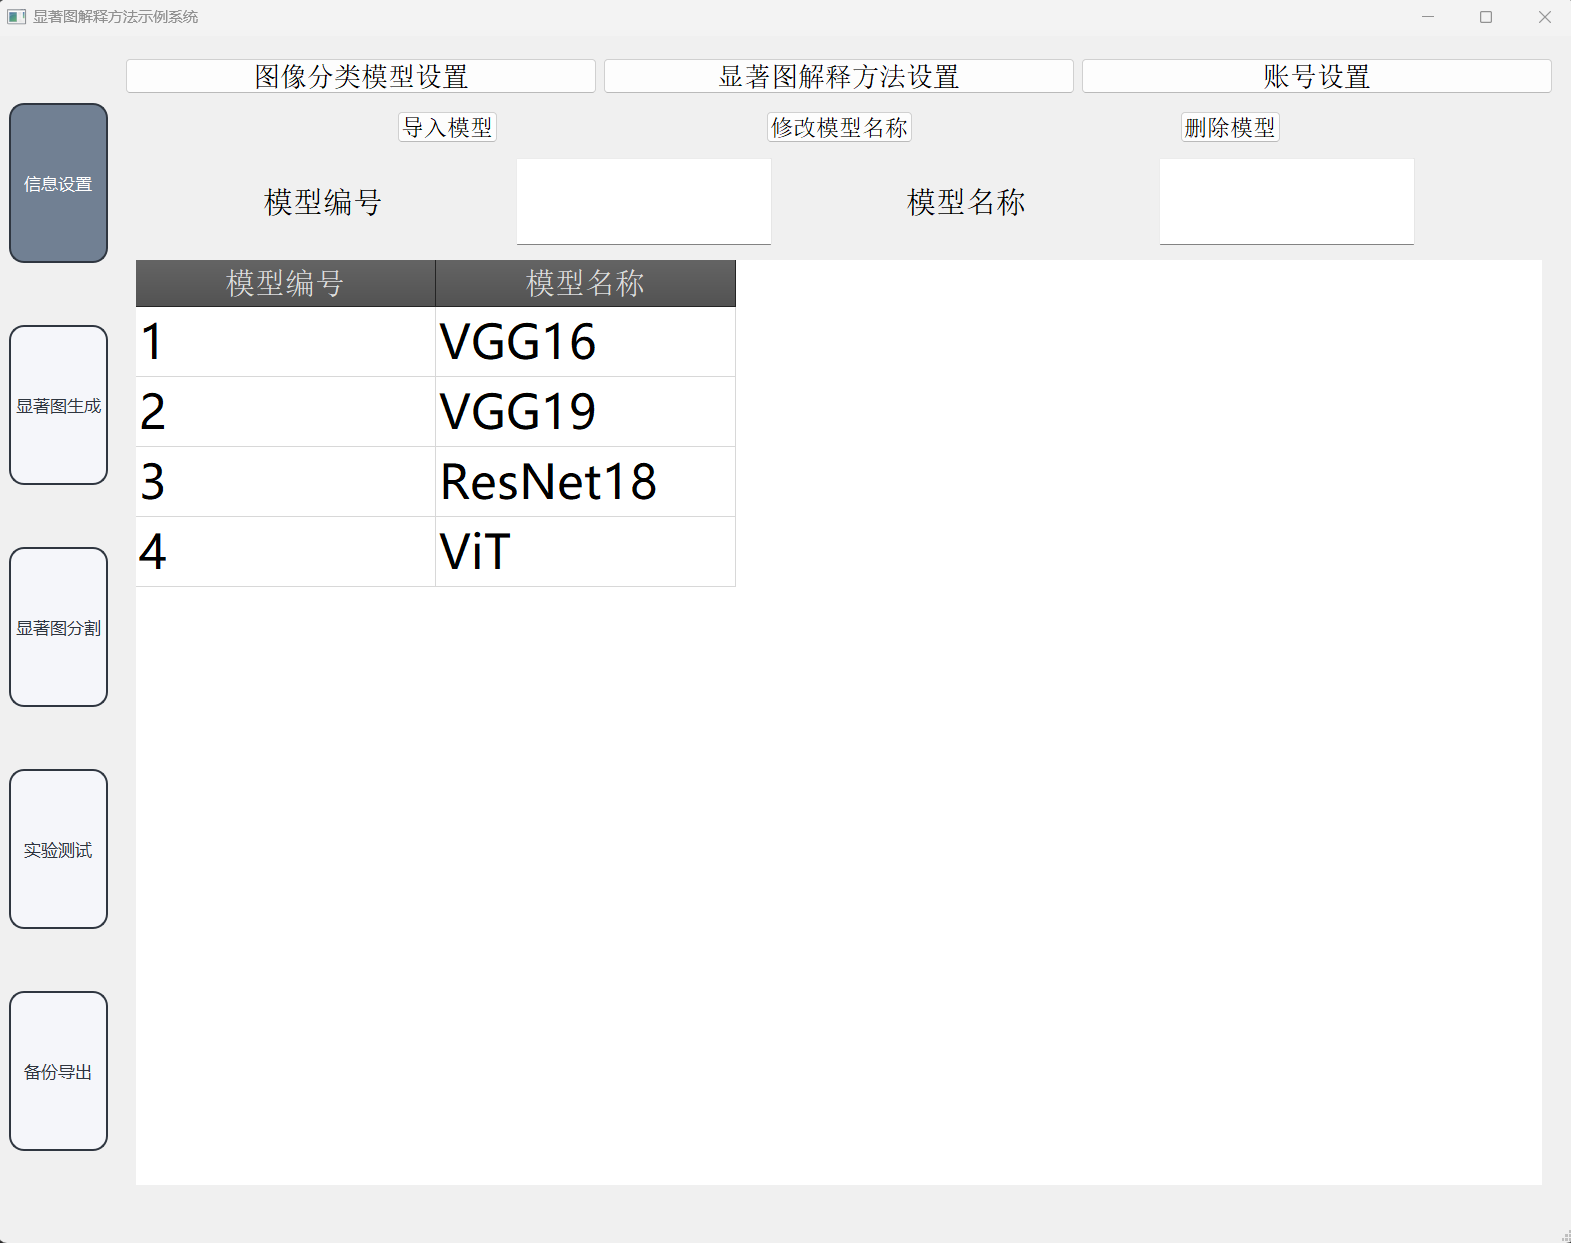
\includegraphics[width=15cm,height=9.5cm]{fig/ch5/f1.png}
	\bicaption[\xiaosi 图像分类模型的查看和导入界面图]{\wuhao 图像分类模型的查看和导入界面图}{\wuhao View and import interface for image classification models}
	\label{fig:f1}
\end{figure}

\begin{figure}[H]
	\centering 
	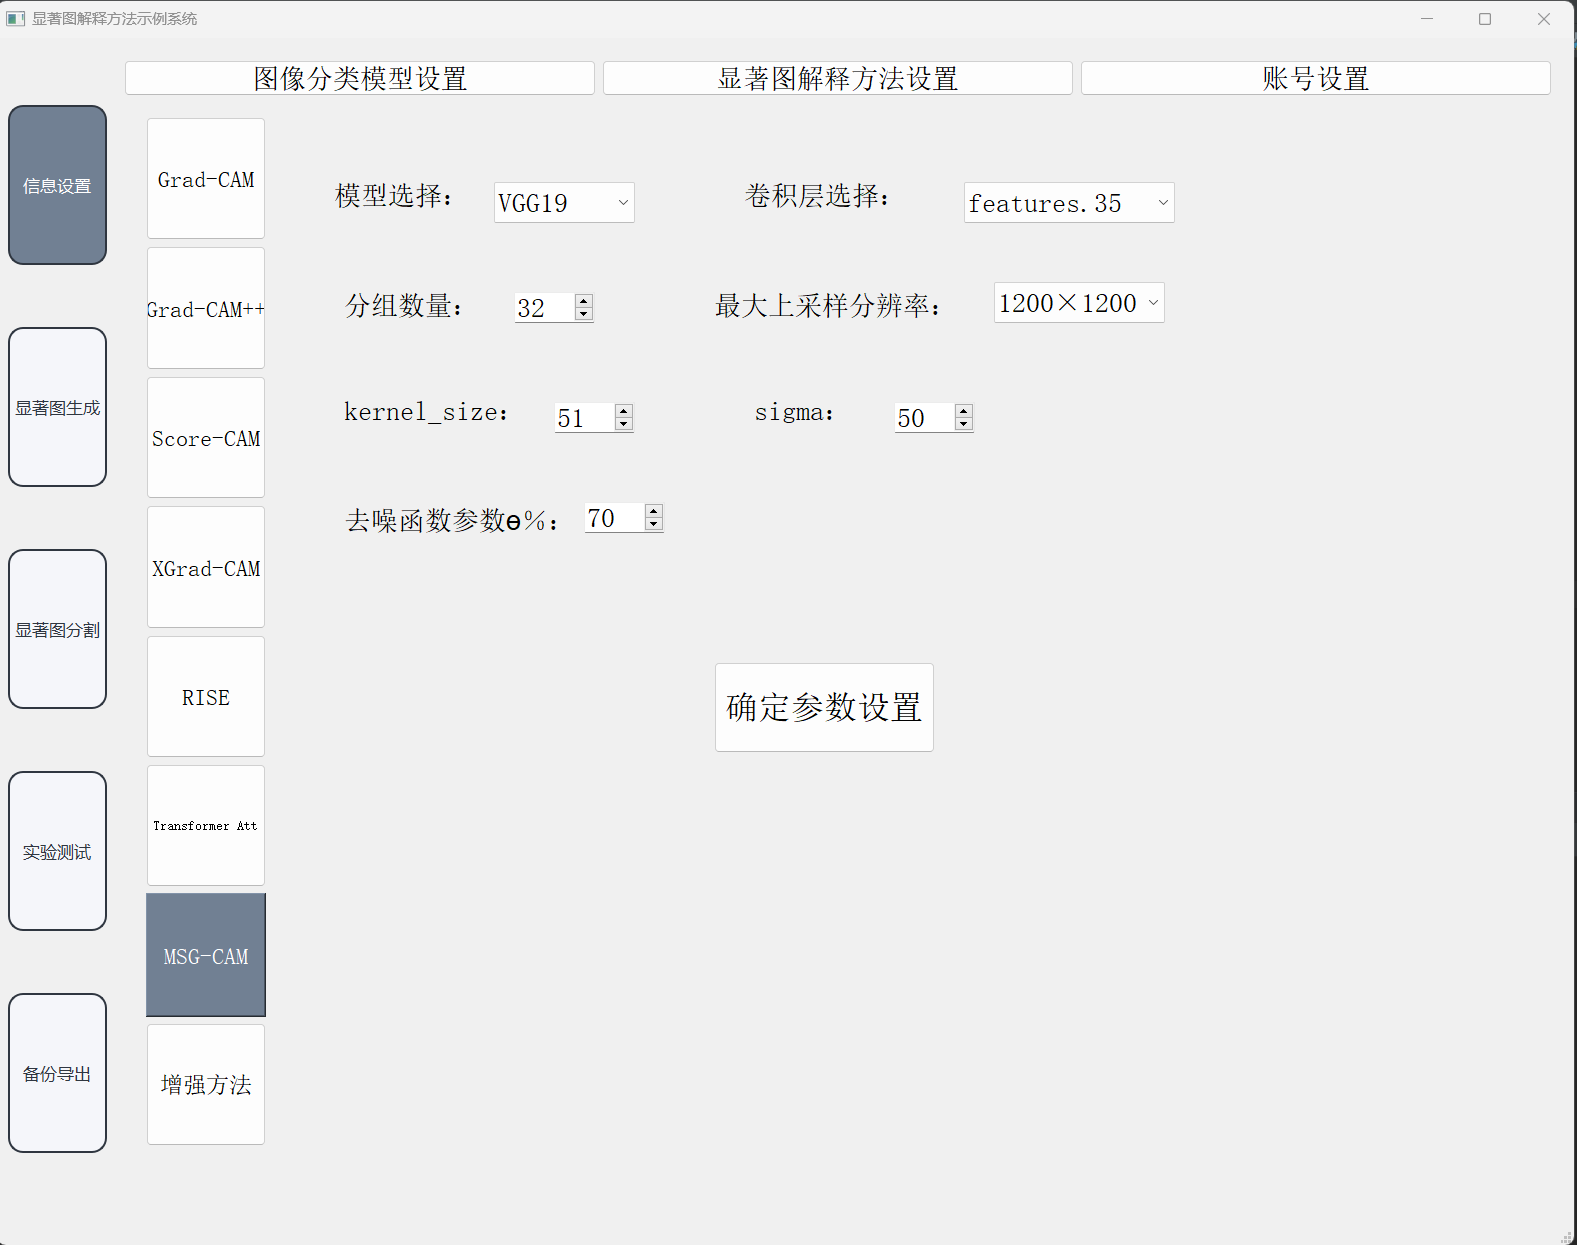
\includegraphics[width=15cm,height=9.5cm]{fig/ch5/f2.png}
	\bicaption[\xiaosi 显著图解释方法参数设置页面]{\wuhao 显著图解释方法参数设置页面}{\wuhao Saliency map method interpretation methods parameter setting page}
	\label{fig:f2}
\end{figure}

\begin{figure}[h]
	\centering 
	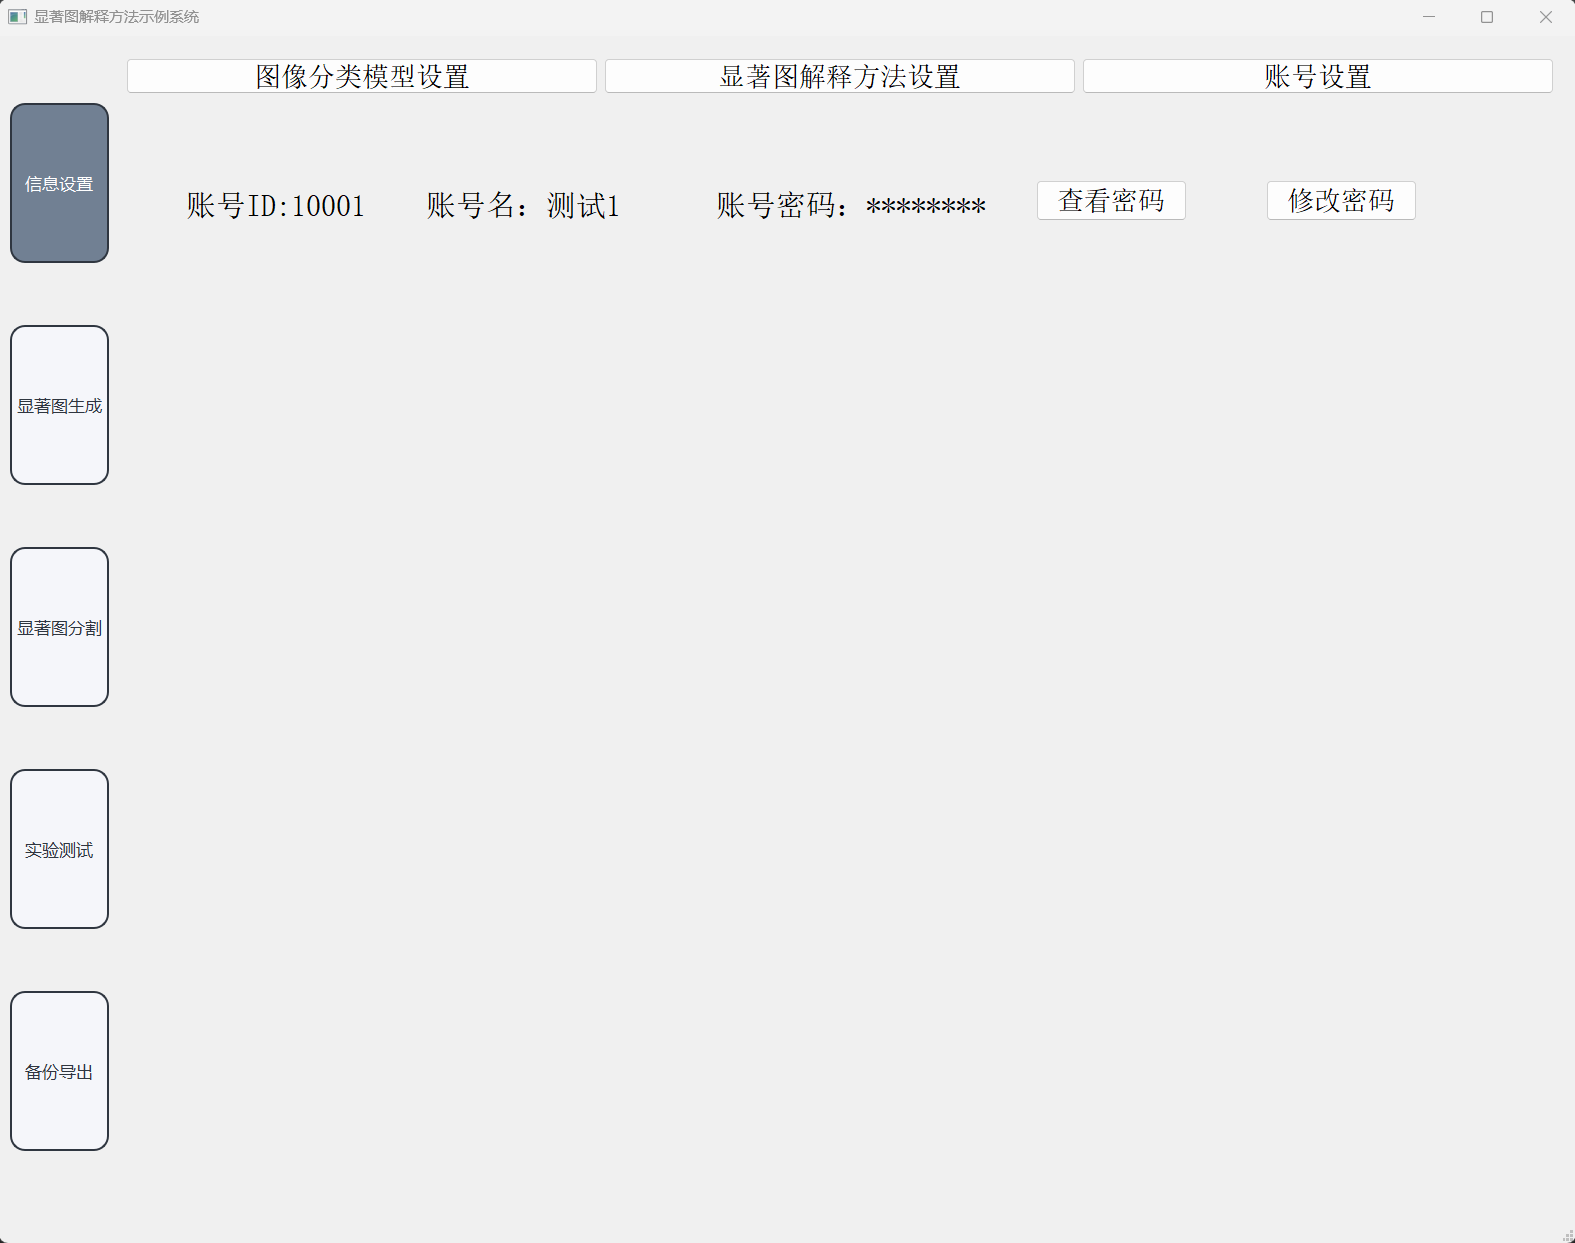
\includegraphics[width=15cm,height=9.5cm]{fig/ch5/f3.png}
	\bicaption[\xiaosi 用户密码修改和查看页面]{\wuhao 用户密码修改和查看页面}{\wuhao User password change and view page}
	\label{fig:f3}
\end{figure}
\begin{figure}[H]
	\centering 
	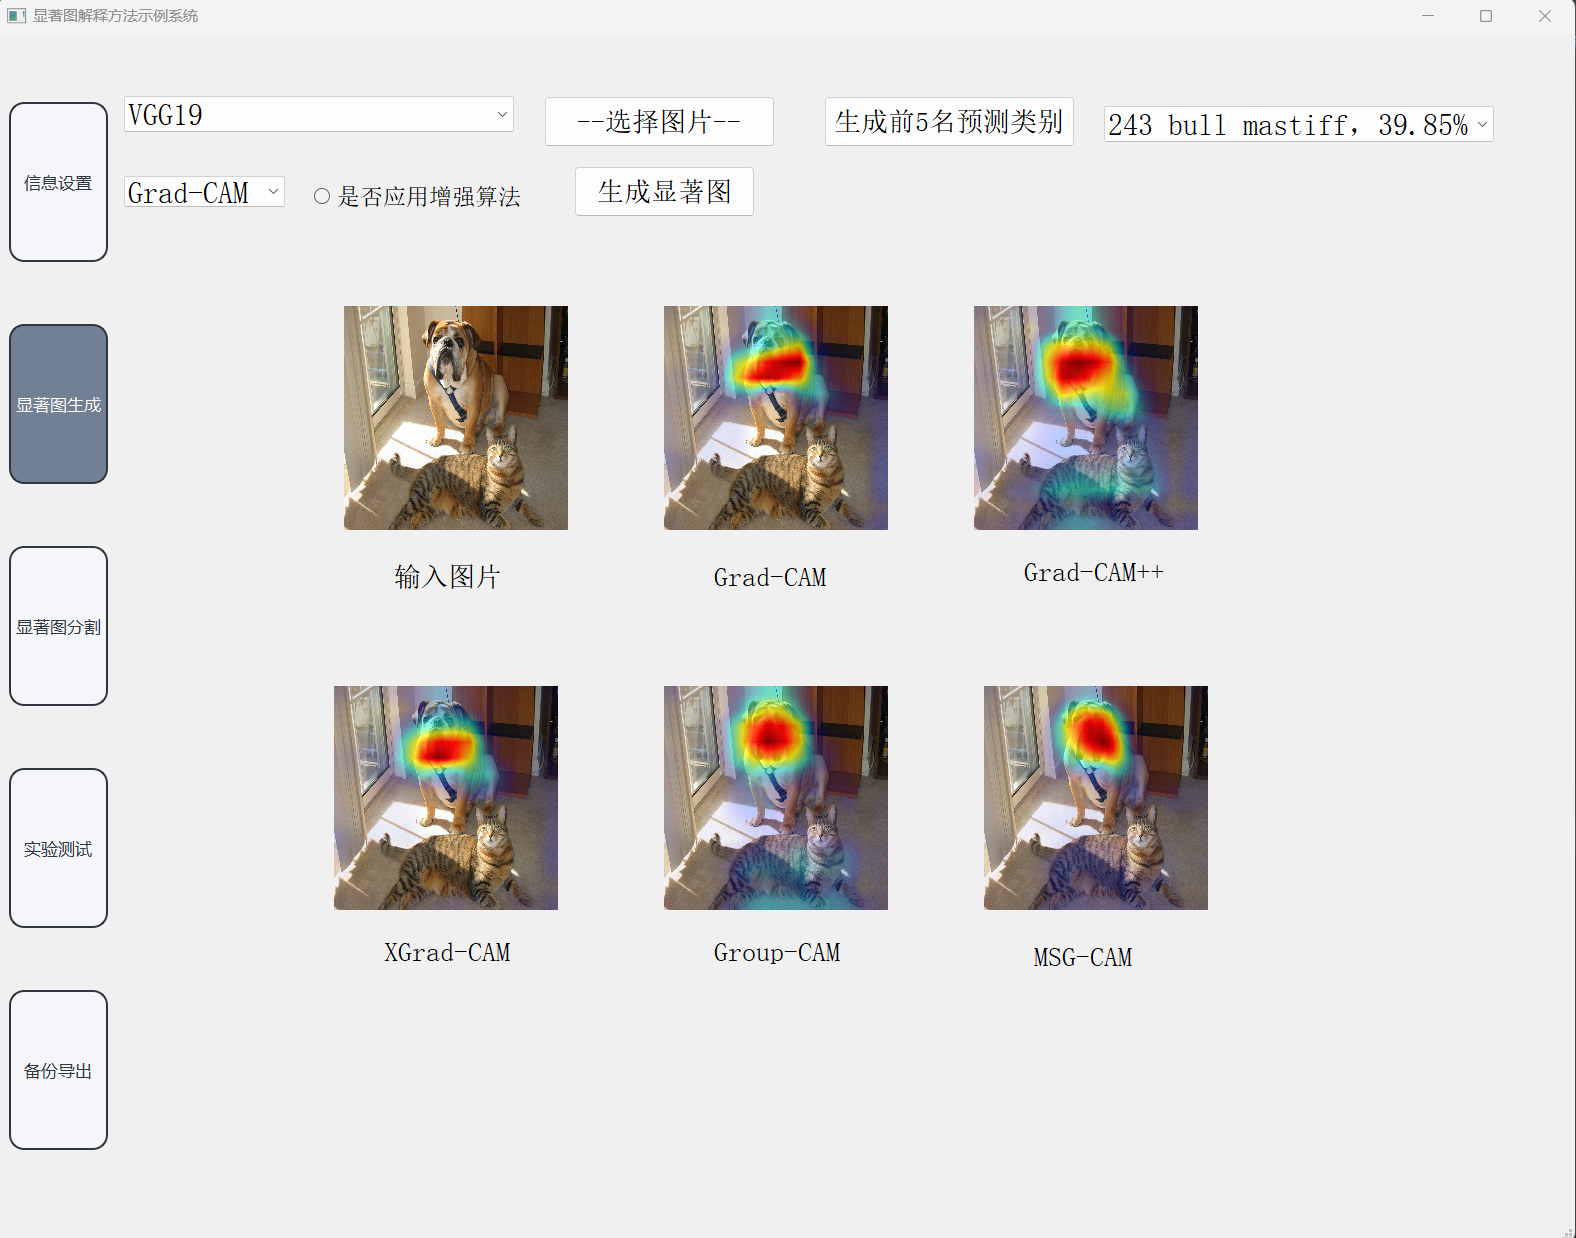
\includegraphics[width=15cm,height=9.5cm]{fig/ch5/f4.png}
	\bicaption[\xiaosi 显著图生成页面]{\wuhao 显著图生成页面}{\wuhao Saliency map generation page}
	\label{fig:f4}
\end{figure}

4.显著图生成功能

在页面截图\ref{fig:f4}中,展示了不同显著图解释方法生成的显著图对比情况,可以看到在选择的输入图片当中,生成了前5名预测类别和相应的概率,用户还可以选择是否应用增强算法来增强该显著图解释方法生成的显著图。


5.显著图分割功能

在图\ref{fig:f5}中展示了根据显著图进行分割情况,在该页面中用户可以设置分割使用的像素比例,选定后生成分割图界面上可以展示分割结果,用户可以直观对比不同方法分割效果,正如该图中展示的那样,在相同分割比例情况下,本文提出的MSG-CAM分割效果更佳,展示了完成的物体,不相关区域更少。

\begin{figure}[h]
	\centering 
	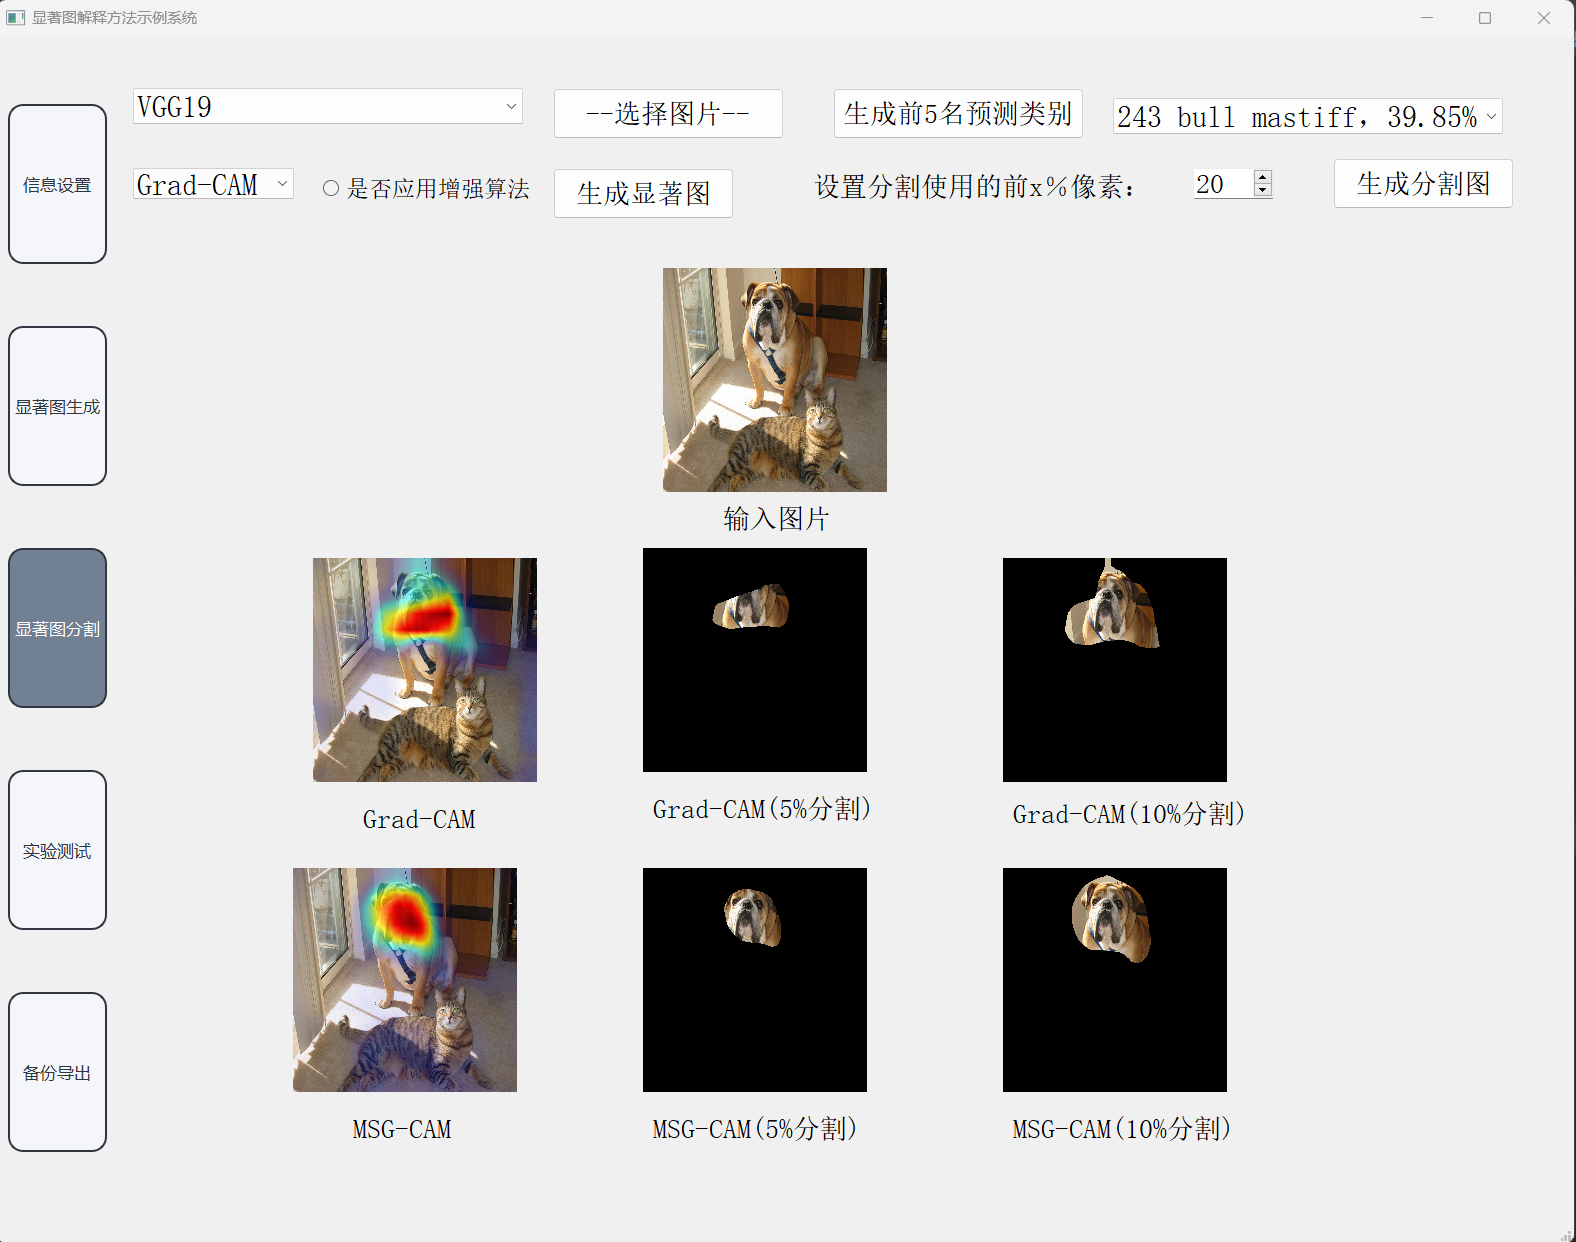
\includegraphics[width=15cm]{fig/ch5/f5.png}
	\bicaption[\xiaosi 显著图分割页面]{\wuhao 显著图分割页面}{\wuhao Saliency map segmentation page}
	\label{fig:f5}
\end{figure}

6.实验评测功能

在图\ref{fig:f6}中展示了实验评测的页面,实验结果通过表格的方式展示在下面页面当中。

\begin{figure}[h]
	\centering 
	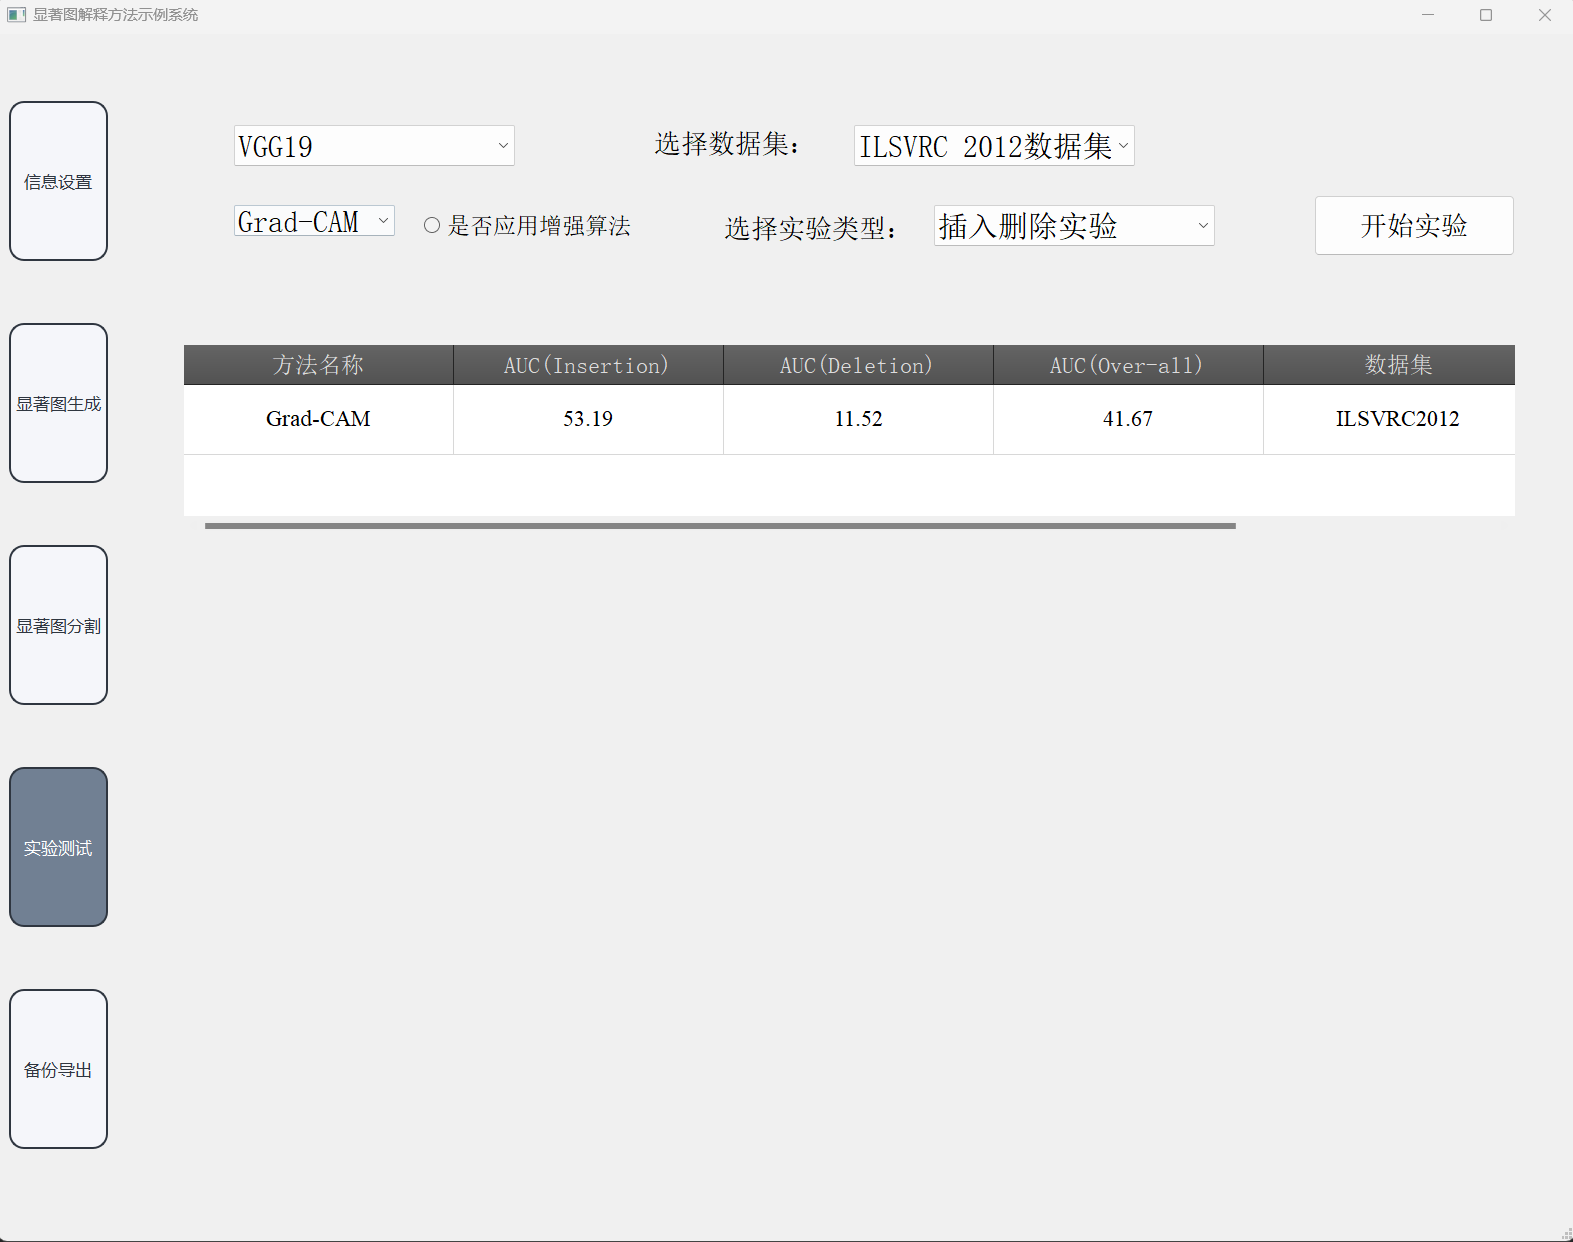
\includegraphics[width=15cm]{fig/ch5/f6.png}
	\bicaption[\xiaosi 实验评测页面]{\wuhao 实验评测页面}{\wuhao Experimental test page}
	\label{fig:f6}
\end{figure}

\section{本章小结}
本章将多种现有的显著图解释方法整合到一个统一的程序接口中,并利用软件可视化开发技术开发了一套显著图解释方法对比评测系统。该系统可以方便研究人员对当前的显著图解释方法进行对比评测,直观展现不同显著图解释方法在相同条件下的视觉差别和评测指标差异。本章通过分析需求和功能设计逐步细化系统功能,并且通过系统页面展示了原型系统的页面功能。

\chapter{总结和展望}
\thispagestyle{others}
\pagestyle{others}
\xiaosi

总结展望


%如果要增加章节数请在此加项

\backmatter

%取消后续章节的页眉上的章节编号
\renewcommand{\chaptermark}[1]{\markboth{#1}{}}

%参考文献

%参考文献



\begin{thebibliography}{200}
\wuhao %设置参考文献字体大小
\linespread{1}\selectfont
\setlength{\itemsep}{-1.4ex} %缩小条目间行距
\thispagestyle{others}
\pagestyle{others}

\makeatletter
\renewcommand\@biblabel[1]{[#1]\hfill} %序号左对齐
\makeatother
\setlength{\labelsep}{0cm}

\bibitem{language}
奚雪峰, 周国栋. 面向自然语言处理的深度学习研究[J]. 自动化学报, 2016,42(10): 1445-1465.

\bibitem{voice}
侯一民, 周慧琼, 王政一. 深度学习在语音识别中的研究进展综述[J]. 计算机应用研究, 2017, 34(8): 2241-2246.

\bibitem{image}
Krizhevsky A, Sutskever I, Hinton G E. Imagenet Classification With Deep Convolutional Neural Networks[J]. Communications of the ACM, 2017, 60(6):84-90

\bibitem{simonyan2014very}
Simonyan K. Very deep convolutional networks for large‐scale image recognition. 3 rd Int Conf learn represent ICLR 2015‐Conf track proc[J]. Published online, 2015: 1.

\bibitem{od1}
Redmon J, Farhadi A. YOLO9000: better, faster, stronger[C] // Proceedings of the IEEE conference on computer vision and pattern recognition. 2017: 7263-7271.
\bibitem{od2}
Ren S, He K, Girshick R, et al. Faster r-cnn: Towards real-time object detection with region proposal networks[J]. Advances in neural information processing systems, 2015, 28.

\bibitem{sg1}
Chen L C, Zhu Y, Papandreou G, et al. Encoder-decoder with atrous separable convolution for semantic image segmentation[C] // Proceedings of the European conference on computer vision (ECCV). 2018: 801-818.
\bibitem{sg2}
Long J, Shelhamer E, Darrell T. Fully convolutional networks for semantic segmentation[C] // Proceedings of the IEEE conference on computer vision and pattern recognition. 2015: 3431-3440.

\bibitem{machine}
Rahwan I, Cebrian M, Obradovich N, et al. Machine Behaviour[J]. Nature,2019, 568(7753): 477-486.

\bibitem{arospace}
Rebuffi S A, Fong R, Ji X, et al. There and back again: Revisiting backpropagation saliency methods[C] // Proceedings of the IEEE/CVF Conference on Computer Vision and Pattern Recognition. 2020: 8839-8848.

\bibitem{post}
Mitros J, Mac Namee B. A Categorisation of Post-Hoc Explanations for Predictive Models[J]. Arxiv Preprint Arxiv:1904.02495, 2019.

\bibitem{post2}
Ras G, Xie N, Van Gerven M, et al. Explainable Deep Learning: A Field Guide for the Uninitiated[J]. Journal of Artificial Intelligence Research, 2022, 73:329-397.

\bibitem{Intrinsic1}
Levy O, Dagan I. Annotating Relation Inference In Context Via Question Answering[C] // Proceedings of the 54th Annual Meeting of the Association for Computational Linguistics (Volume 2: Short Papers), Berlin, Germany, 2016:249-255.

\bibitem{Intrinsic2}
Yoon J, Jordon J, Van Der Schaar M. INVASE: Instance-Wise Variable Selection Using Neural Networks[C] // International Conference on Learning Representations, New Orleans, Louisiana, United States, 2018: 4857-4881.

\bibitem{Intrinsic3}
Kim J, Rohrbach A, Darrell T, et al. Textual Explanations for Self-Driving Vehicles[C] // Proceedings of the European Conference on Computer Vision (ECCV), Munich, GERMANY, 2018: 563-578.

\bibitem{Intrinsic4}
Chang S, Zhang Y, Yu M, et al. A Game Theoretic Approach to Class-Wise Selective Rationalization[J]. Advances in Neural Information Processing Systems, 2019, 32: 10055-10065.
\bibitem{Intrinsic5}
Zhang Q, Wu Y N, Zhu S C. Interpretable Convolutional Neural Networks[C] // Proceedings of the IEEE Conference on Computer Vision and Pattern Recognition Salt Lake City, UT, USA, 2018: 8827-8836.
\bibitem{Intrinsic6}
Elsayed G, Kornblith S, Le Q V. Saccader: Improving Accuracy of Hard Attention Models for Vision[J]. Advances in Neural Information Processing Systems, 2019, 32: 700-712.

\bibitem{zeiler2014visualizing}
Zeiler M D, Fergus R. Visualizing and understanding convolutional networks[C] // Computer Vision–ECCV 2014: 13th European Conference, Zurich, Switzerland, September 6-12, 2014, Proceedings, Part I 13. Springer International Publishing, 2014: 818-833.

\bibitem{springenberg2014striving}
Springenberg J T, Dosovitskiy A, Brox T, et al. Striving for simplicity: The all convolutional net[J/OL]. arXiv preprint arXiv:1412.6806, 2014.

\bibitem{shrikumar2017learning}
Shrikumar A, Greenside P, Kundaje A. Learning important features through propagating activation differences[C] // International conference on machine learning. PMLR, 2017: 3145-3153.

\bibitem{binder2016layer}
Binder A, Montavon G, Lapuschkin S, et al. Layer-wise relevance propagation for neural networks with local renormalization layers[C] // Artificial Neural Networks and Machine Learning–ICANN 2016: 25th International Conference on Artificial Neural Networks, Barcelona, Spain, September 6-9, 2016, Proceedings, Part II 25. Springer International Publishing, 2016: 63-71.

\bibitem{simonyan2014deep}
Simonyan K, Vedaldi A, Zisserman A. Deep inside convolutional networks: Visualising image classification models and saliency maps[J/OL]. arXiv preprint arXiv:1312.6034, 2013.

\bibitem{smilkov2017smoothgrad}
Smilkov D, Thorat N, Kim B, et al. Smoothgrad: removing noise by adding noise[J/OL]. arXiv preprint arXiv:1706.03825, 2017.

\bibitem{adebayo2018local}
Adebayo J, Gilmer J, Goodfellow I, et al. Local explanation methods for deep neural networks lack sensitivity to parameter values[J]. arXiv preprint arXiv:1810.03307, 2018.

\bibitem{sundararajan2017axiomatic}
Sundararajan M, Taly A, Yan Q. Axiomatic attribution for deep networks[C] // International conference on machine learning. PMLR, 2017: 3319-3328.

\bibitem{adebayo2018sanity}
Adebayo J, Gilmer J, Muelly M, et al. Sanity checks for saliency maps[J]. Advances in neural information processing systems, 2018, 31.

\bibitem{zhou2016learning}
Zhou B, Khosla A, Lapedriza A, et al. Learning deep features for discriminative localization[C] // Proceedings of the IEEE conference on computer vision and pattern recognition. 2016: 2921-2929.

\bibitem{selvaraju2017grad}
Selvaraju R R, Cogswell M, Das A, et al. Grad-cam: Visual explanations from deep networks via gradient-based localization[C] // Proceedings of the IEEE international conference on computer vision. 2017: 618-626.

\bibitem{chattopadhay2018grad}
Chattopadhay A, Sarkar A, Howlader P, et al. Grad-cam++: Generalized gradient-based visual explanations for deep convolutional networks[C] // 2018 IEEE winter conference on applications of computer vision (WACV). IEEE, 2018: 839-847.

\bibitem{fu2020axiom}
Fu R, Hu Q, Dong X, et al. Axiom-based grad-cam: Towards accurate visualization and explanation of cnns[J]. arXiv preprint arXiv:2008.02312, 2020.

\bibitem{omeiza2019smooth}
Omeiza D, Speakman S, Cintas C, et al. Smooth grad-cam++: An enhanced inference level visualization technique for deep convolutional neural network models[J]. arXiv preprint arXiv:1908.01224, 2019.

\bibitem{wang2020ss}
Wang H, Naidu R, Michael J, et al. SS-CAM: Smoothed Score-CAM for sharper visual feature localization[J]. arXiv preprint arXiv:2006.14255, 2020.

\bibitem{ramaswamy2020ablation}
Ramaswamy H G. Ablation-cam: Visual explanations for deep convolutional network via gradient-free localization[C] // proceedings of the IEEE/CVF winter conference on applications of computer vision. 2020: 983-991.

\bibitem{wang2020score}
Wang H, Wang Z, Du M, et al. Score-CAM: Score-weighted visual explanations for convolutional neural networks[C] // Proceedings of the IEEE/CVF conference on computer vision and pattern recognition workshops. 2020: 24-25.

\bibitem{lee2021relevance}
Lee J R, Kim S, Park I, et al. Relevance-cam: Your model already knows where to look[C] // Proceedings of the IEEE/CVF Conference on Computer Vision and Pattern Recognition. 2021: 14944-14953.

\bibitem{jalwana2021cameras}
Jalwana M A A K, Akhtar N, Bennamoun M, et al. CAMERAS: Enhanced resolution and sanity preserving class activation mapping for image saliency[C] // Proceedings of the IEEE/CVF Conference on Computer Vision and Pattern Recognition. 2021: 16327-16336.

\bibitem{lundberg2017unified}
Lundberg S M, Lee S I. A unified approach to interpreting model predictions[J]. Advances in neural information processing systems, 2017, 30.

\bibitem{ribeiro2016should}
Ribeiro M T, Singh S, Guestrin C. " Why should i trust you?" Explaining the predictions of any classifier[C] // Proceedings of the 22nd ACM SIGKDD international conference on knowledge discovery and data mining. 2016: 1135-1144.

\bibitem{petsiuk2018rise}
Petsiuk V, Das A, Saenko K. Rise: Randomized input sampling for explanation of black-box models[J]. arXiv preprint arXiv:1806.07421, 2018.

\bibitem{fong2019understanding}
Fong R, Patrick M, Vedaldi A. Understanding deep networks via extremal perturbations and smooth masks[C] // Proceedings of the IEEE/CVF international conference on computer vision. 2019: 2950-2958.
\bibitem{fong2017interpretable}
Fong R C, Vedaldi A. Interpretable explanations of black boxes by meaningful perturbation[C] // Proceedings of the IEEE international conference on computer vision. 2017: 3429-3437.

\bibitem{ILSVRC}
Russakovsky O, Deng J, Su H, et al. Imagenet large scale visual recognition challenge[J]. International journal of computer vision, 2015, 115: 211-252.
\bibitem{pascal}
Everingham M, Van Gool L, Williams C K I, et al. The pascal visual object classes (voc) challenge[J]. International journal of computer vision, 2010, 88: 303-338.
\bibitem{coco}
Lin T Y, Maire M, Belongie S, et al. Microsoft coco: Common objects in context[C] // Computer Vision–ECCV 2014: 13th European Conference, Zurich, Switzerland, September 6-12, 2014, Proceedings, Part V 13. Springer International Publishing, 2014: 740-755.

\bibitem{bengio2013representation}
Bengio Y, Courville A, Vincent P. Representation learning: A review and new perspectives[J]. IEEE transactions on pattern analysis and machine intelligence, 2013, 35(8): 1798-1828.

\bibitem{vaswani2017attenion}
Vaswani A, Shazeer N, Parmar N, et al. Attention is all you need[J]. Advances in neural information processing systems, 2017, 30.
\bibitem{kenton2019bert}
Kenton J D M W C, Toutanova L K. BERT: Pre-training of Deep Bidirectional Transformers for Language Understanding[C]//Proceedings of NAACL-HLT. 2019: 4171-4186.
\bibitem{floridi2020gpt}
Floridi L, Chiriatti M. GPT-3: Its nature, scope, limits, and consequences[J]. Minds and Machines, 2020, 30: 681-694.

\bibitem{dosovitskiy2020image}
Dosovitskiy A, Beyer L, Kolesnikov A, et al. An image is worth 16x16 words: Transformers for image recognition at scale[J]. arXiv preprint arXiv:2010.11929, 2020.

\bibitem{chefer2021transformer}
Chefer H, Gur S, Wolf L. Transformer interpretability beyond attention visualization[C] // Proceedings of the IEEE/CVF conference on computer vision and pattern recognition. 2021: 782-791.

\bibitem{mahendran2016visualizing}
Mahendran A, Vedaldi A. Visualizing deep convolutional neural networks using natural pre-images[J]. International Journal of Computer Vision, 2016, 120: 233-255.

\bibitem{simonyan2014visualising}
Simonyan K, Vedaldi A, Zisserman A. Visualising image classification models and saliency maps[J]. Deep Inside Convolutional Networks, 2014, 2.



\bibitem{montavon2017explaining}
Montavon G, Lapuschkin S, Binder A, et al. Explaining nonlinear classification decisions with deep taylor decomposition[J]. Pattern recognition, 2017, 65: 211-222.


\bibitem{zhang2021novel}
Zhang Q, Rao L, Yang Y. A novel visual interpretability for deep neural networks by optimizing activation maps with perturbation[C] // Proceedings of the AAAI Conference on Artificial Intelligence. 2021, 35(4): 3377-3384.

\bibitem{kapishnikov2019xrai}
Kapishnikov A, Bolukbasi T, Viégas F, et al. Xrai: Better attributions through regions[C] // Proceedings of the IEEE/CVF International Conference on Computer Vision. 2019: 4948-4957.

\bibitem{dabkowski2017real}
Dabkowski P, Gal Y. Real time image saliency for black box classifiers[J]. Advances in neural information processing systems, 2017, 30.

\bibitem{zhang2018top}
Zhang J, Bargal S A, Lin Z, et al. Top-down neural attention by excitation backprop[J]. International Journal of Computer Vision, 2018, 126(10): 1084-1102.

\bibitem{guillaumin2014imagenet}
Guillaumin M, Küttel D, Ferrari V. Imagenet auto-annotation with segmentation propagation[J]. International Journal of Computer Vision, 2014, 110: 328-348.



\end{thebibliography}

%\bibliographystyle{unsrt}


% 此参考文献名为ref.bib文件

%\bibliography{ref}
%\thispagestyle{others}





\clearpage

%如果没有附录请自行删除以下页面

%附录A
%%\specialsectioning
\chapter{附录A 各学院中英文名称对照表}
\thispagestyle{others}

\begin{table}[h]
	\renewcommand{\arraystretch}{1.5}
	\centering
	\begin{tabular}{p{2cm}p{3cm}p{8.5cm}}
		\toprule[1.5pt]
		\makecell[c]{\songti\xiaosi\bfseries 序号}&\makecell[l]{\songti\xiaosi\bfseries 中文名称}&\makecell[l]{\songti\xiaosi\bfseries 英文名称}\\
		\hline
		\makecell[c]{\wuhao 01}&\makecell[l]{\wuhao 通信工程学院}&\makecell[c]{\wuhao School of Communications and Information Engineering}\\
		\bottomrule[1.5pt]
	\end{tabular}
	
\end{table}

\clearpage
%
%%附录B
%%\specialsectioning
\chapter{附录B 常见一级学科中英文名称对照表}
\thispagestyle{others}



\begin{table}[h]
	\renewcommand{\arraystretch}{1.5}
	\centering
	\begin{tabular}{p{2cm}p{3cm}p{8.5cm}}
		\toprule[1.5pt]
		\makecell[c]{\songti\xiaosi\bfseries 代码}&\makecell[l]{\songti\xiaosi\bfseries 中文名称}&\makecell[l]{\songti\xiaosi\bfseries 英文名称}\\
		\hline
		\makecell[c]{\wuhao 0810}&\makecell[l]{\wuhao 信息与通信工程}&\makecell[l]{\wuhao Information and Communication Engineering}\\
		\bottomrule[1.5pt]
	\end{tabular}
	
\end{table}

\clearpage
%
%%附录C
%%\specialsectioning

\chapter{附录C 常见专业学位类别中英文名称对照表}

\thispagestyle{others}


\begin{table}[h]
	\renewcommand{\arraystretch}{1.5}
	\centering
	\begin{tabular}{p{2cm}p{3cm}p{8.5cm}}
		\toprule[1.5pt]
		\makecell[c]{\songti\xiaosi\bfseries 代码}&\makecell[l]{\songti\xiaosi\bfseries 中文名称}&\makecell[l]{\songti\xiaosi\bfseries 英文名称}\\
		\hline
		\makecell[c]{\wuhao 1256}&\makecell[l]{\wuhao 工程管理}&\makecell[l]{\wuhao Engineering Management}\\
		\bottomrule[1.5pt]
	\end{tabular}
	
\end{table}

\clearpage

%作者简介
\specialsectioning


\chapter{作者简介}
\thispagestyle{others}
\pagestyle{others}
\xiaosi

\section{1. \ 基本情况}
张涪源,男,四川人,1998年10月出生,重庆邮电大学计算机科学与技术学院计算机技术专业2021级硕士研究生。

\section{2. \ 教育和工作经历}



2017.09~2021.06 南京林业大学信息科学技术学院,本科,专业:软件工程

2021.09~2024.09 重庆邮电大学计算机科学与技术学院,硕士研究生,专业:计算机技术

\section{3. \ 攻读学位期间的研究成果}

\subsection{3.1 \ 发表的学术论文和著作}
\hangafter 1
\hangindent 1.5em
\noindent
[1] \textbf{Zhang F}, Xiang X, Deng X, et al. Multi-size scaled CAM for more accurate visual interpretation of CNNs[C]. International Conference on Neural Computing for Advanced Applications, NCAA2023, Hefei, China, 2023: 147-161.(EI会议,已发表)

\hangafter 1
\hangindent 1.5em
\noindent
[2] Xiang X, \textbf{Zhang F}, Deng X, et al. MSG-CAM: Multi-scale inputs make a better visual interpretation of CNN networks[C]. 2023 IEEE International Conference on Multimedia and Expo (ICME), Brisbane, Australia, 2023: 312-317.(CCF-B类会议,已发表)

\hangafter 1
\hangindent 1.5em
\noindent
[3] Xiang X, \textbf{Zhang F}, Deng X, et al. Visualization enhancement of saliency methods based on the sliding window mechanism[C]. 26th European Conference on Artificial Intelligence ECAI 2023, Kraków, Poland, 2023: 2728-2735.(CCF-B类会议,已发表)

\subsection{3.2 \ 申请(授权)专利}

\hangafter 1
\hangindent 1.5em
\noindent
[1]项小红,\textbf{张涪源},邓欣,丁晓宇.一种基于上采样机制和类激活映射的图像分类结果特征可视化方法.中国,CN202310400157.2[P].2023.04.14.(已受理)

\hangafter 1
\hangindent 1.5em
\noindent
[2] 项小红,\textbf{张涪源},邓欣,张浩.一种基于滑动窗口机制的图像分类神经网络可视化算法的增强方法.中国,CN202310428053.2[P].2023.07.07.(已受理)










% 致谢
% 致谢
%\specialsectioning
\chapter{致 \quad 谢}
\thispagestyle{others}
\pagestyle{others}
\xiaosi

感谢老师、同学们的关心、支持和帮助!

感谢老师、同学们的关心、支持和帮助!

感谢老师、同学们的关心、支持和帮助!

感谢老师、同学们的关心、支持和帮助!

感谢老师、同学们的关心、支持和帮助!

感谢老师、同学们的关心、支持和帮助!

感谢老师、同学们的关心、支持和帮助!

感谢老师、同学们的关心、支持和帮助!

感谢老师、同学们的关心、支持和帮助!

感谢老师、同学们的关心、支持和帮助!

感谢老师、同学们的关心、支持和帮助!

感谢老师、同学们的关心、支持和帮助!

感谢老师、同学们的关心、支持和帮助!

感谢老师、同学们的关心、支持和帮助!

感谢老师、同学们的关心、支持和帮助!

感谢老师、同学们的关心、支持和帮助!

感谢老师、同学们的关心、支持和帮助!

感谢老师、同学们的关心、支持和帮助!

感谢老师、同学们的关心、支持和帮助!

感谢老师、同学们的关心、支持和帮助!

感谢老师、同学们的关心、支持和帮助!

感谢老师、同学们的关心、支持和帮助!

感谢老师、同学们的关心、支持和帮助!

感谢老师、同学们的关心、支持和帮助!

感谢老师、同学们的关心、支持和帮助!

感谢老师、同学们的关心、支持和帮助!

感谢老师、同学们的关心、支持和帮助!

感谢老师、同学们的关心、支持和帮助!

感谢老师、同学们的关心、支持和帮助!

感谢老师、同学们的关心、支持和帮助!

感谢老师、同学们的关心、支持和帮助!

感谢老师、同学们的关心、支持和帮助!

感谢老师、同学们的关心、支持和帮助!

感谢老师、同学们的关心、支持和帮助!

感谢老师、同学们的关心、支持和帮助!

感谢老师、同学们的关心、支持和帮助!

感谢老师、同学们的关心、支持和帮助!

感谢老师、同学们的关心、支持和帮助!

感谢老师、同学们的关心、支持和帮助!

感谢老师、同学们的关心、支持和帮助!

感谢老师、同学们的关心、支持和帮助!

感谢老师、同学们的关心、支持和帮助!

感谢老师、同学们的关心、支持和帮助!







\end{document}